\documentclass[a4paper]{article}
%\documentclass[journal]{IEEEtran}


\usepackage[utf8]{inputenc}
\usepackage[T1]{fontenc}
\usepackage{textcomp}
\usepackage[italian]{babel}
\usepackage{amsmath, amssymb}
\usepackage{siunitx}
\usepackage{caption}
\usepackage{graphicx}
\usepackage{subcaption}
\usepackage{amsmath}
\usepackage{darkmode}
%\enabledarkmode
\usepackage{booktabs} % Opzionale, per tabelle più belle se vuoi (\toprule, \midrule, \bottomrule)
\usepackage{ragged2e} % Per \Centering nelle minipage
\usepackage{float} % Per [htbp]

% ======================================================
% Impostazioni siunitx (opzionale, ma utile)
% ======================================================
\sisetup{
    output-decimal-marker = {,}, % Usa la virgola come separatore decimale
    uncertainty-mode = separate, % Mostra incertezza come ±
    separate-uncertainty = true, % Forza la separazione
    locale = IT % Impostazioni locali italiane (es. per la virgola)
}

% ======================================================
% Appendice con le tabelle dati
% ======================================================
\usepackage{appendix} % Usa il pacchetto appendix per una gestione migliore
\usepackage{titling}
\usepackage{appendix} % Pacchetto per l'appendice
\usepackage[colorlinks=true, linkcolor=blue, citecolor=blue, urlcolor=blue]{hyperref} % Per riferimenti cliccabili (opzionale ma utile)
\renewcommand{\appendixname}{Appendice} % Traduce "Appendix" in "Appendice"
\renewcommand{\appendixtocname}{Appendici} % Traduce "Appendices" nel ToC
\renewcommand{\appendixpagename}{Appendici} % Traduce "Appendices" nell'header/footer
\title{Circuiti 2 - Turno 2A - Gruppo 29}
\author{Alessio Ramirez \and Michele Rota \and Sofia Zocchi}
\date{4 Aprile 2025}
\begin{document}
\maketitle
\tableofcontents
\newpage

\section{Circuito RC}
\subsection{Obiettivo}
Studiare l'andamento della differenza di potenziale ai capi di un resistore e di un condensatore inseriti in un circuito RC in funzione del tempo. Valutare sia la fase di carica che di scarica del circuito, alimentato da un segnale di tensione ad onda quadra.
\subsection{Metodo}
\begin{center}
	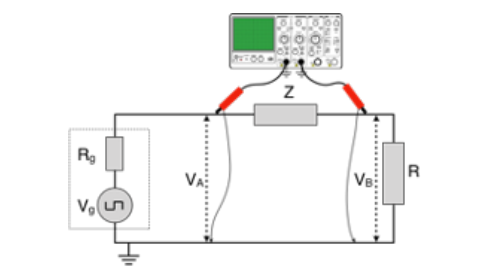
\includegraphics[width=0.5\textwidth]{grafici/circuito-rc.png}
	\captionof{figure}{Circuito RC}
	\label{fig:rc_circuito}
\end{center}
Per poter effettuare le misurazioni abbiamo dapprima realizzato il circuito, sulla base dello schema riportato in figura \ref{fig:rc_circuito}. In questo caso $Z$ indica la capacità $C$. Per poter campionare la forma d'onda di $V_c (t)$ e $V_R (t)$ abbiamo utilizzato un oscilloscopio a cui sono state collegate due sonde. Una sonda è stata posizionata in modo tale da misurare l'andamento di $V_g$, segnale ad onda quadra, e l'altra è stata invece spostata a seconda delle esigenze di misurazione: prima ai capi della capacità e poi della resistenza. A partire dai valori noti di $C$ e $R$ abbiamo stimato la costante di tempo caratteristica del circuito $\tau$, mediante la relazione \( \mathit{\tau = RC} \), in modo tale da poter impostare una frequenza $f$ dell'onda quadra che ci permettesse di osservare una carica/scarica completa del circuito. In quanto \(\tau \approx 10^{-3} s\) abbiamo imposto $f = 100 Hz$, così che il periodo dell'onda quadra \( \mathit{T = \frac{1}{f} = 10^{-2} s}\) risultasse $\approx10\tau$.
Sulla base dell'analisi circuitale (legge delle maglie e relazioni caratteristiche per ciascun componente del circuito) abbiamo ricavato le relazioni necessarie ad interpolare l'andamento di $V_c (t)$ e $V_r (t)$.
Più precisamente abbiamo ottenuto:
\begin{align}
	 & V_c(t) = V_g(1-\frac{2e^-\frac{t}{\mathit{\tau}}}{1+e^-\frac{T}{\mathit{2\tau}}})  \quad \text{e} \quad V_R(t) = (\frac{2V_g}{1+e^-\frac{T}{\mathit{2\tau}}})e^{-\frac{t}{\mathit{\tau}}}\quad \label{eq:rc_full} % Cambiato label
\end{align}
Poichè \( \mathit{T\approx10 \mathit{\tau}} \), possiamo considerare \( \mathit{e^-\frac{T}{2\tau}}\approx 0 \) , dunque possiamo descrivere più semplicemente il circuito mediante le relazioni:
\begin{align}
	& V_c(t) = V_g(1-2e^{-\frac{t}{\mathit{\tau}}})  \quad \text{e} \quad V_R(t) = 2V_ge^{-\frac{t}{\mathit{\tau}}}\quad \label{eq:rc_approx} % Cambiato label
\end{align}

\subsection{Dati}
Tanto per la fase di carica quanto per quella di scarica abbiamo raccolto circa 30 misure delle coppie \( \mathit{V_c-t} \) e \( \mathit{V_R-t} \). Abbiamo stimato l'incertezza sulle misure utilizzando la sensibilità degli strumenti, ossia la precisione della scala impostata per la visualizzazione dei dati sull'oscilloscopio.
Nelle Tabelle \ref{tab:rc_data_carica_c} e \ref{tab:rc_data_scarica_c} (Appendice \ref{app:dati_rc}) sono raccolti i valori della differenza di potenziale ai capi della capacità al variare del tempo.
Nelle Tabelle \ref{tab:rc_data_carica_r} e \ref{tab:rc_data_scarica_r} (Appendice \ref{app:dati_rc}) abbiamo invece i valori della differenza di potenziale ai capi della resistenza misurata a tempi successivi.

% Le tabelle dati sono state spostate in appendice

\subsection{Analisi dati}
I dati sono stati interpolati utilizzando le relazioni riportate in precenza (Eq. \ref{eq:rc_approx}). I risultati ottenuti dai fit sono riportati nelle Tabella \ref{tab:rc_fit_results}. Questi risultati, in particolare i valori di $\tau$ ricavati sperimentalmente ($\tau_s$), sono stati utilizzati per calcolare la costante di tempo caratteristica del circuito.

\begin{center}
    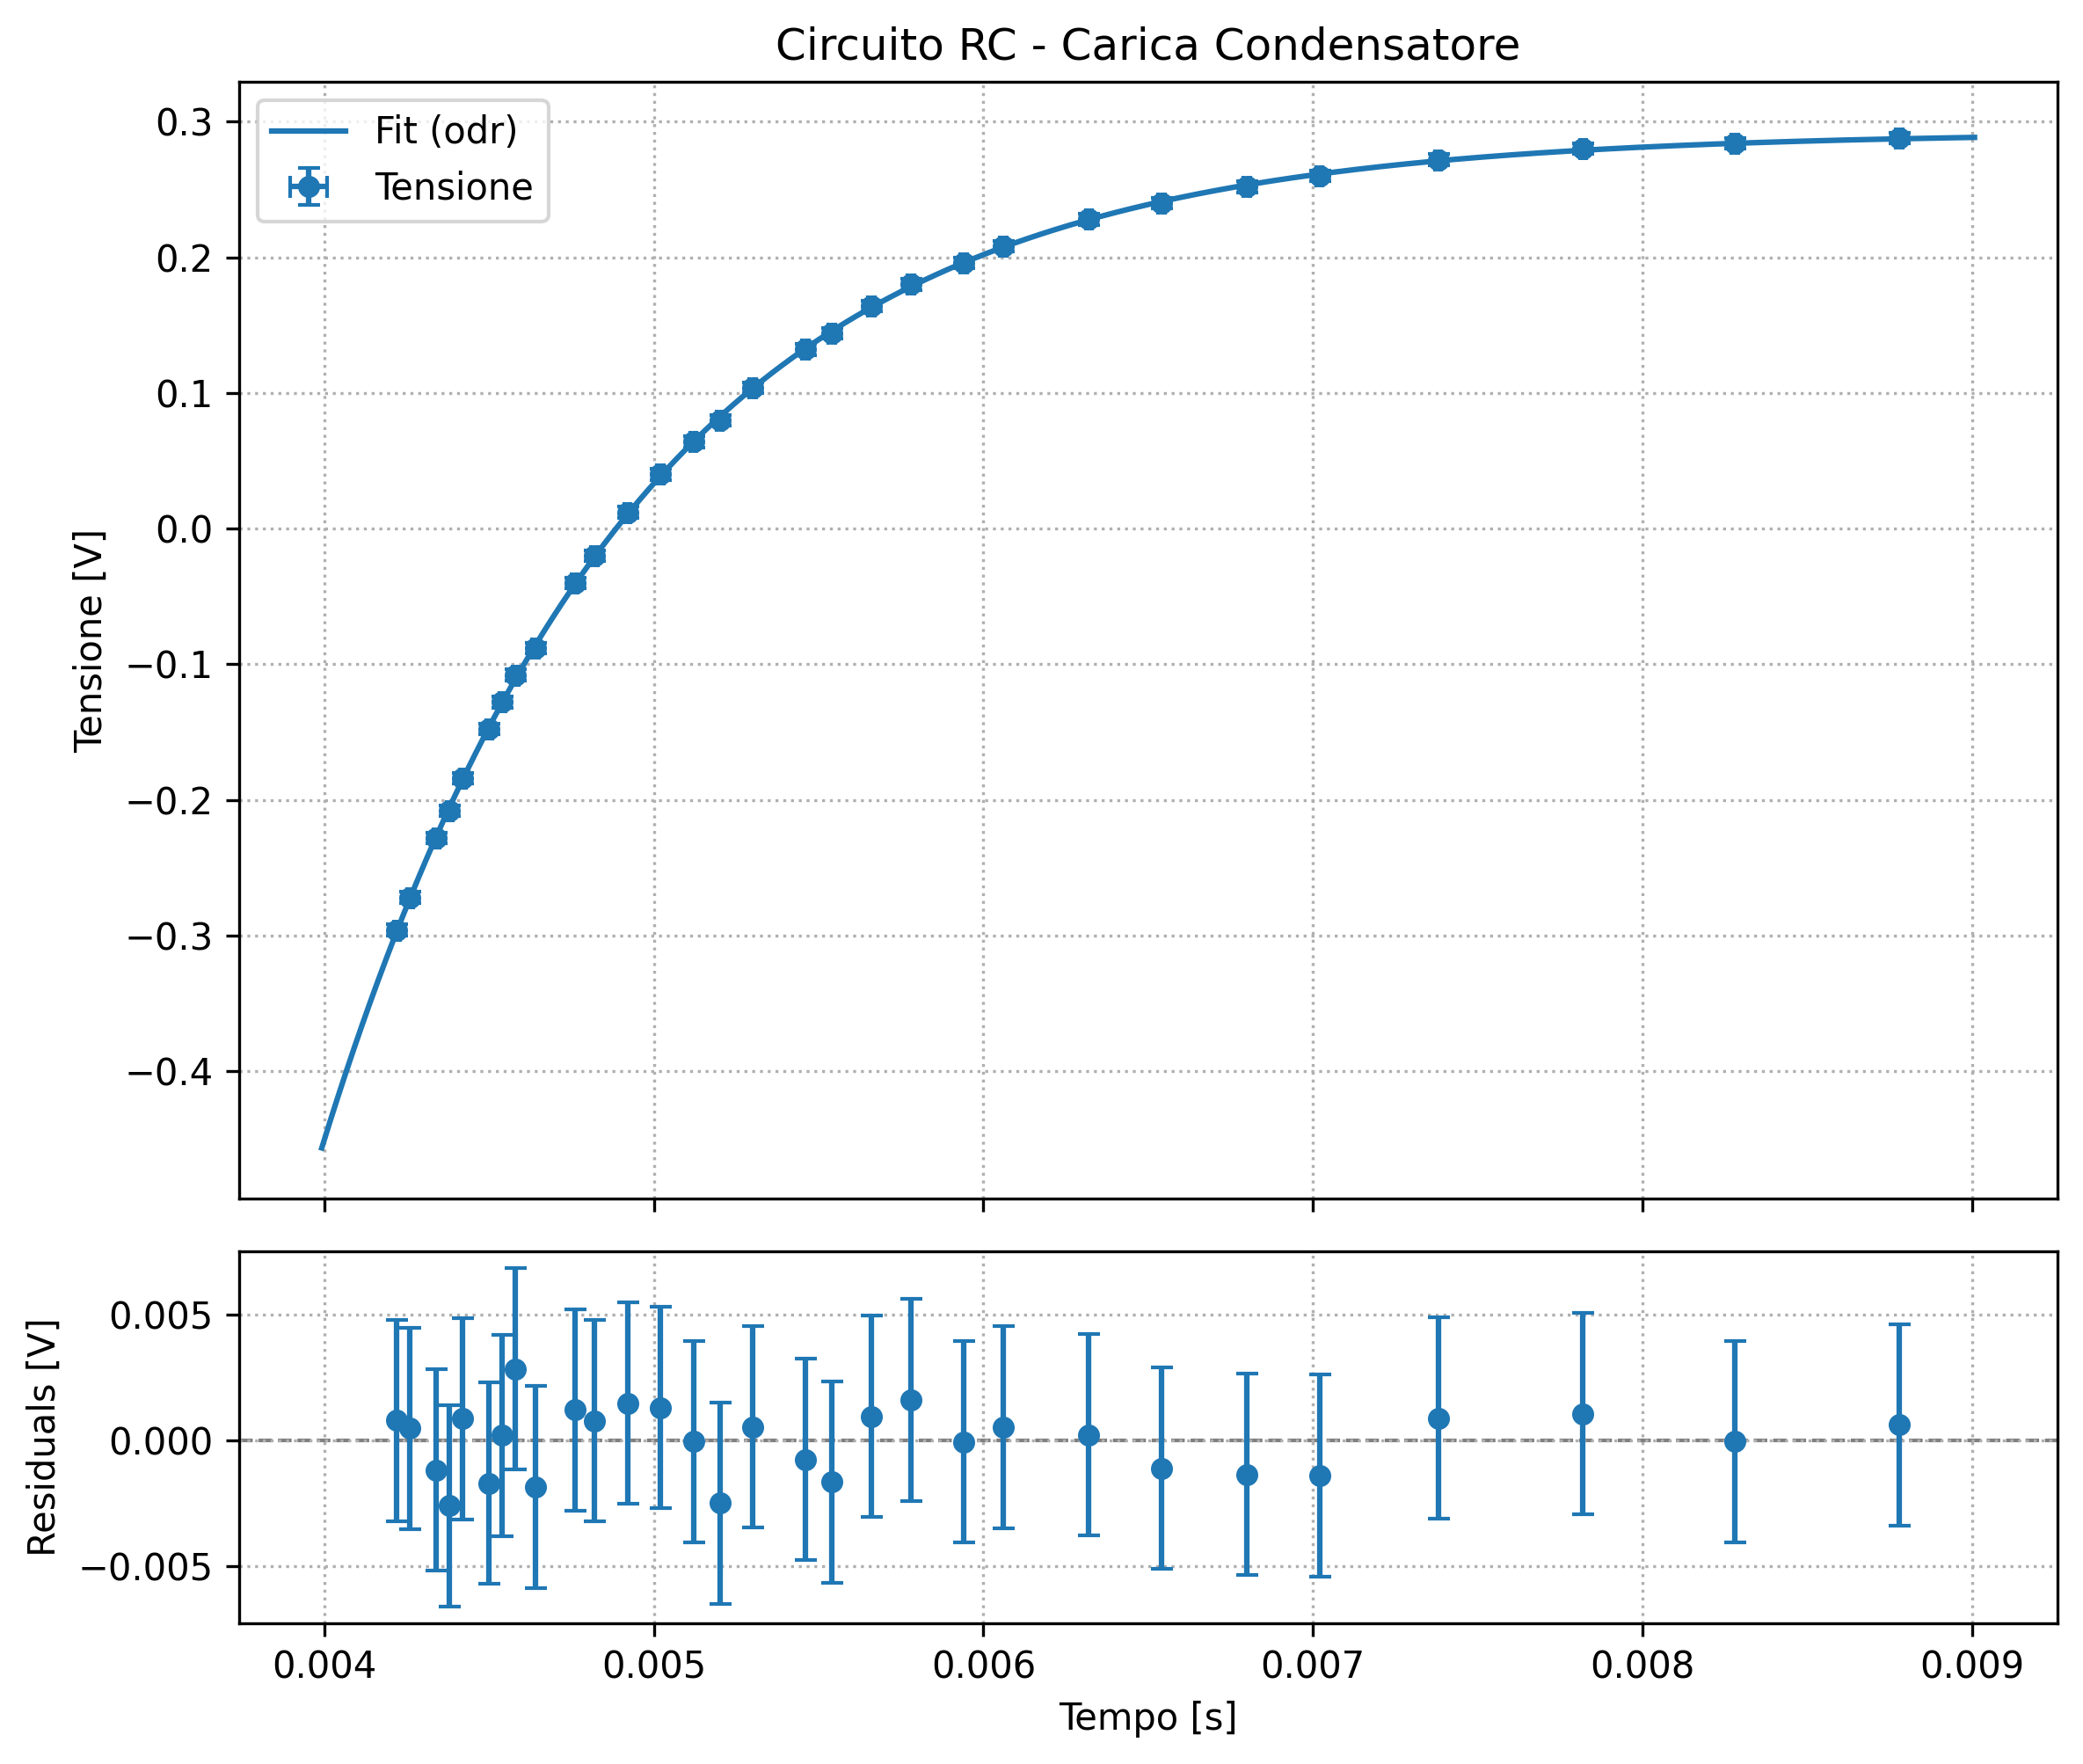
\includegraphics[width=0.9\linewidth]{grafici/rc_carica_condensatore.png}
    \captionof{figure}{Carica condensatore - Dati e Fit}
    \label{fig: rc carica condensatore}
    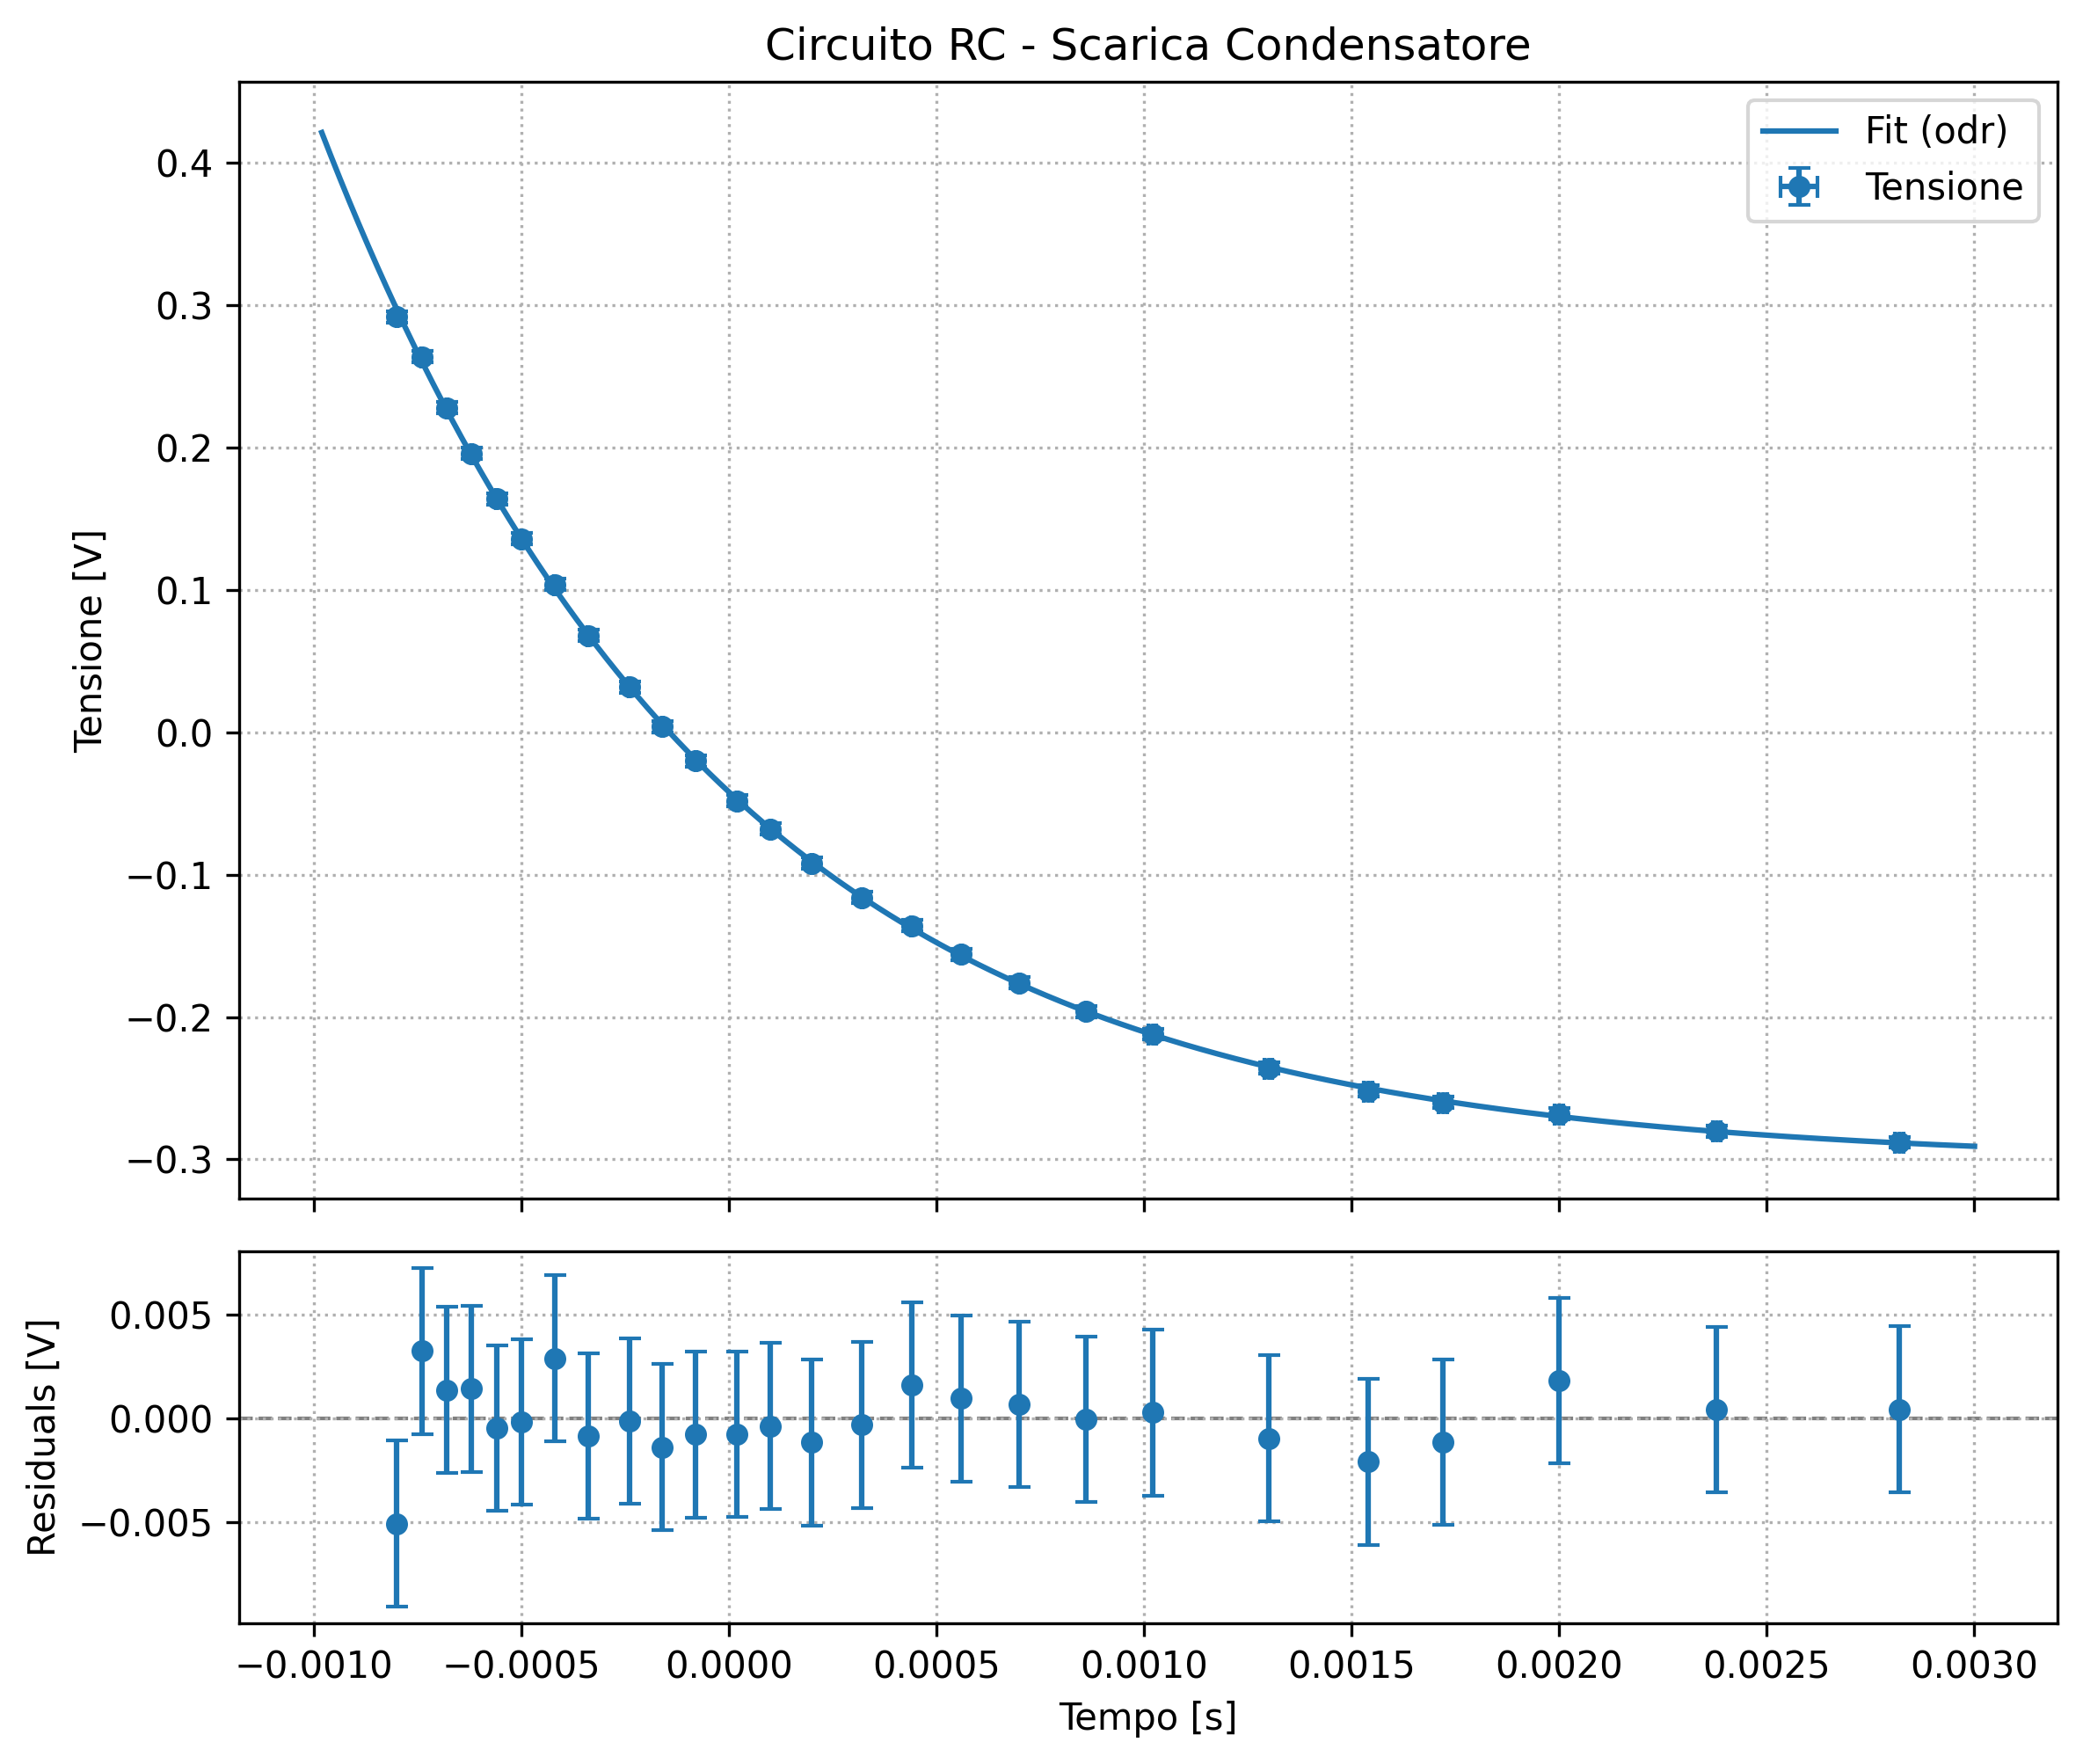
\includegraphics[width=0.9\linewidth]{grafici/rc_scarica_condensatore.png}
    \captionof{figure}{Scarica condensatore - Dati e Fit}
    \label{fig: rc scarica condensatore}
    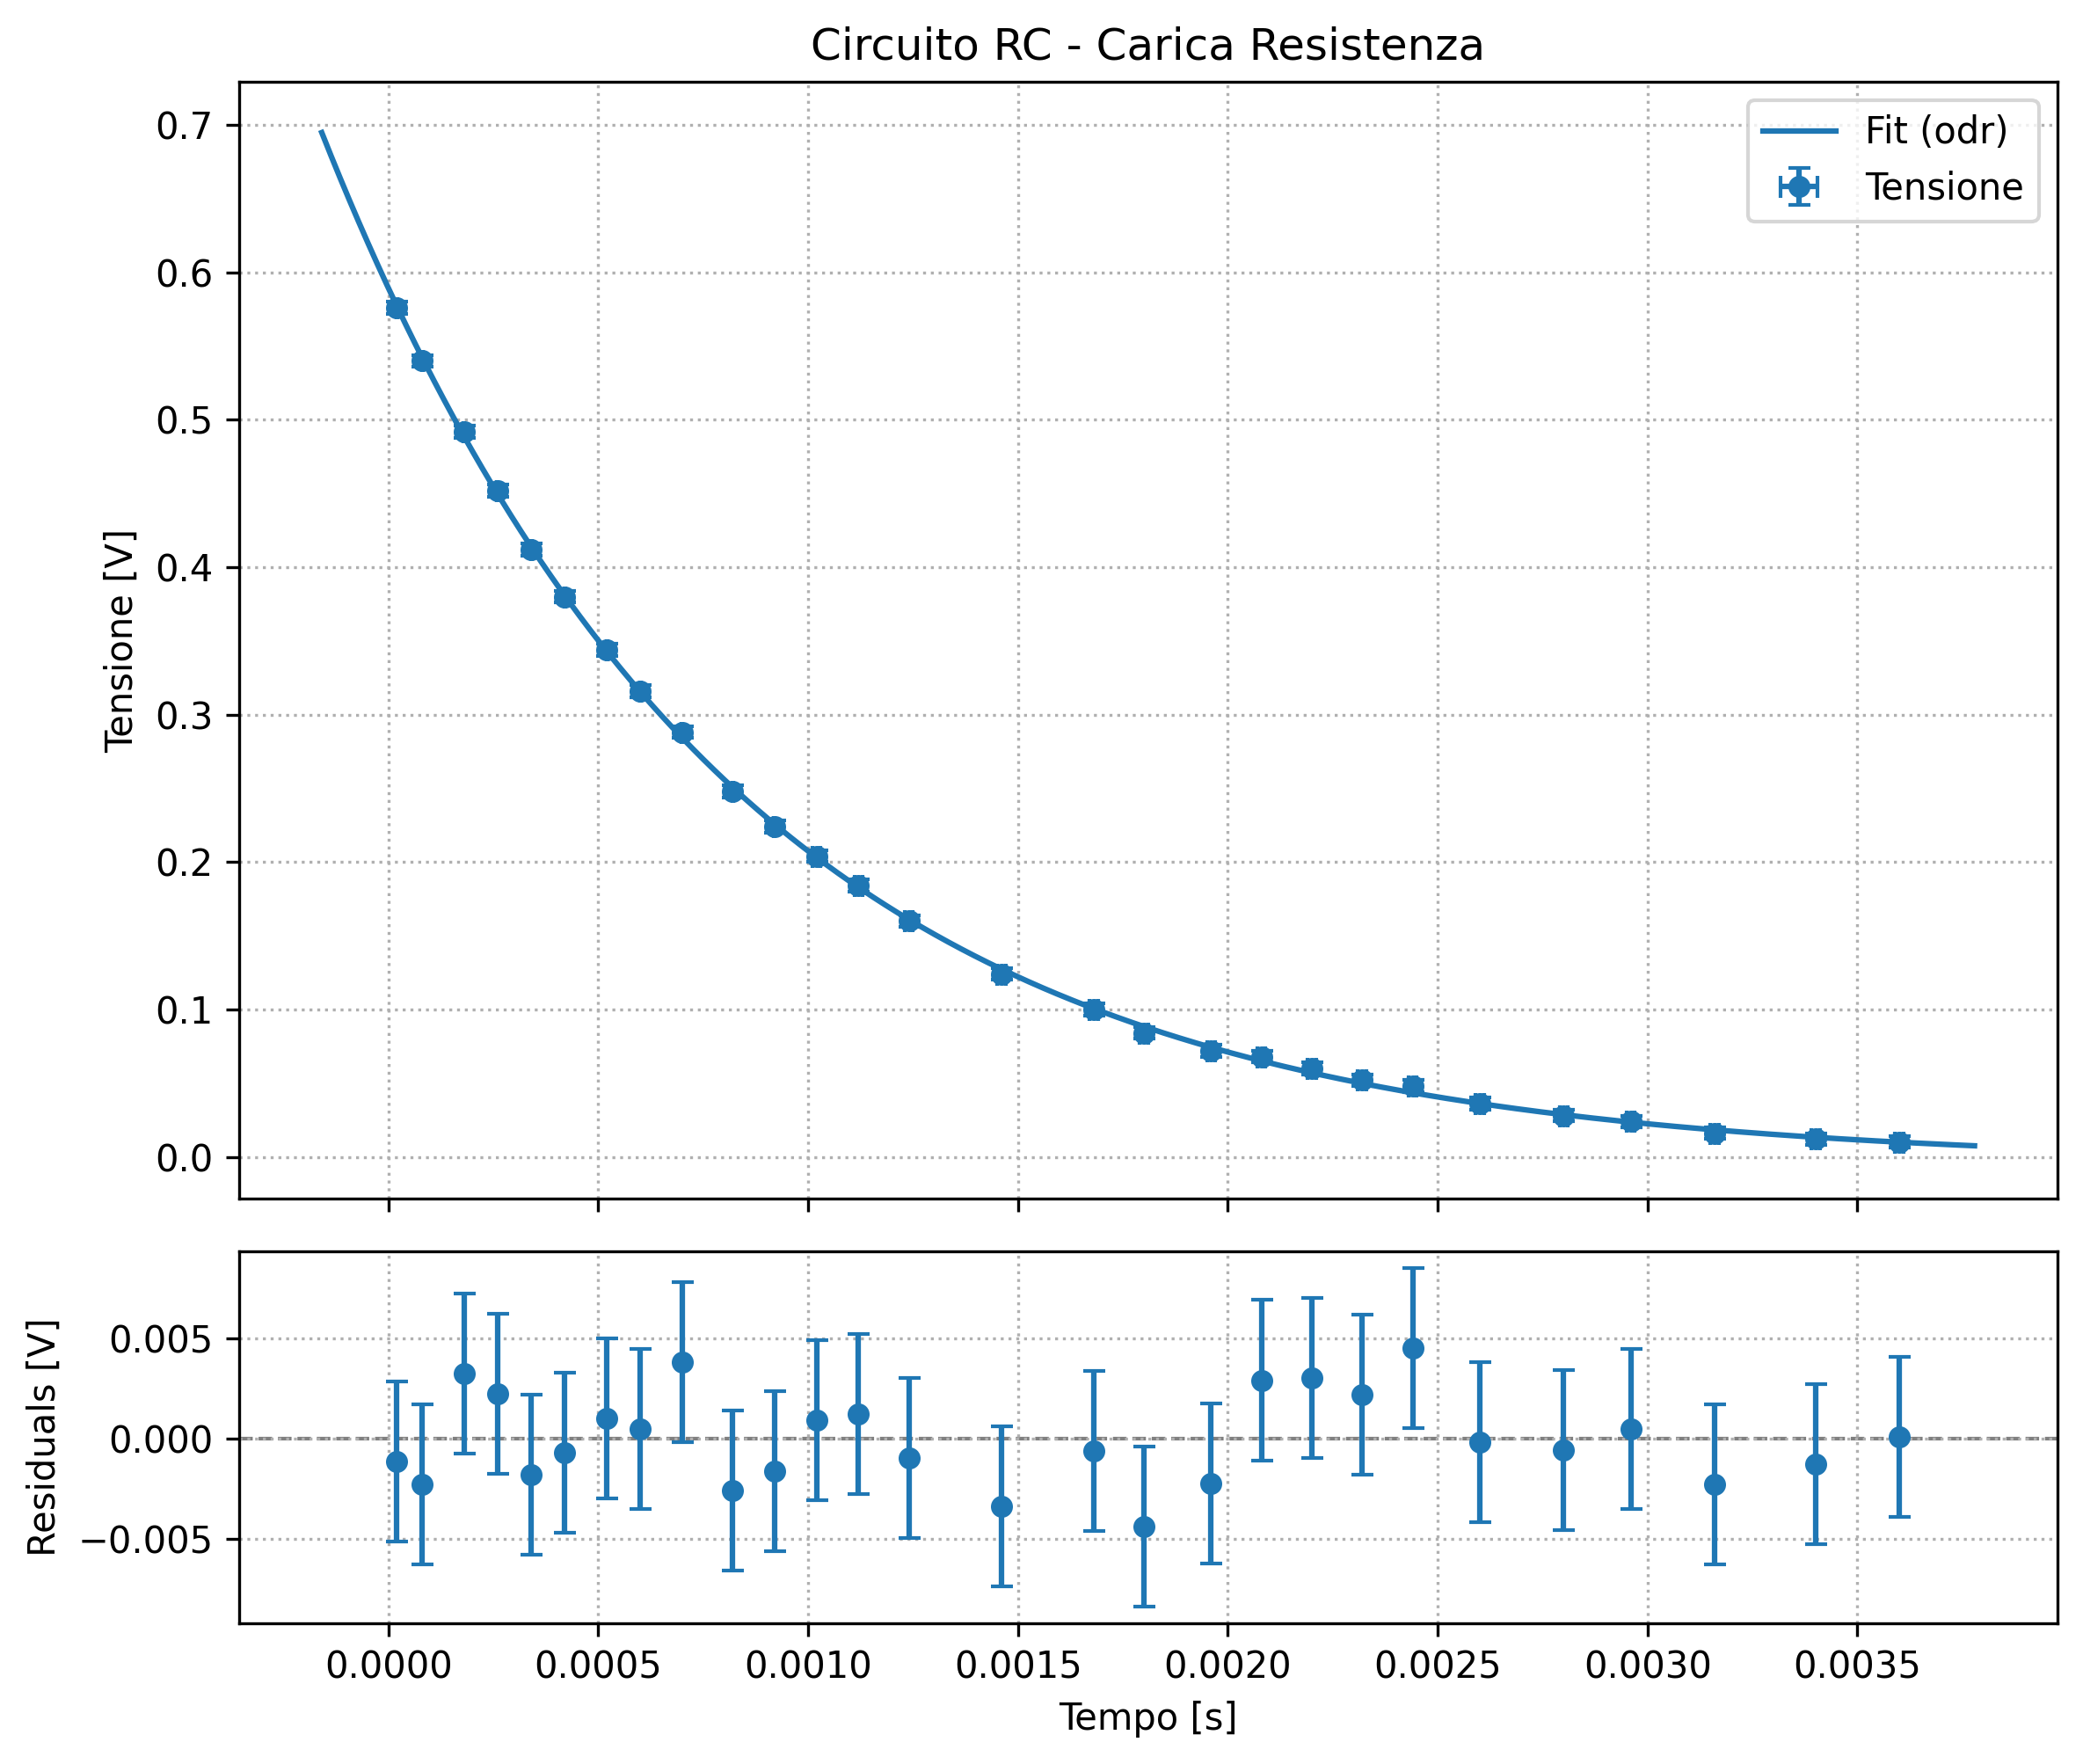
\includegraphics[width=0.9\linewidth]{grafici/rc_carica_resistenza.png}
    \captionof{figure}{Carica resistenza - Dati e Fit}
    \label{fig: rc carica resistenza}
    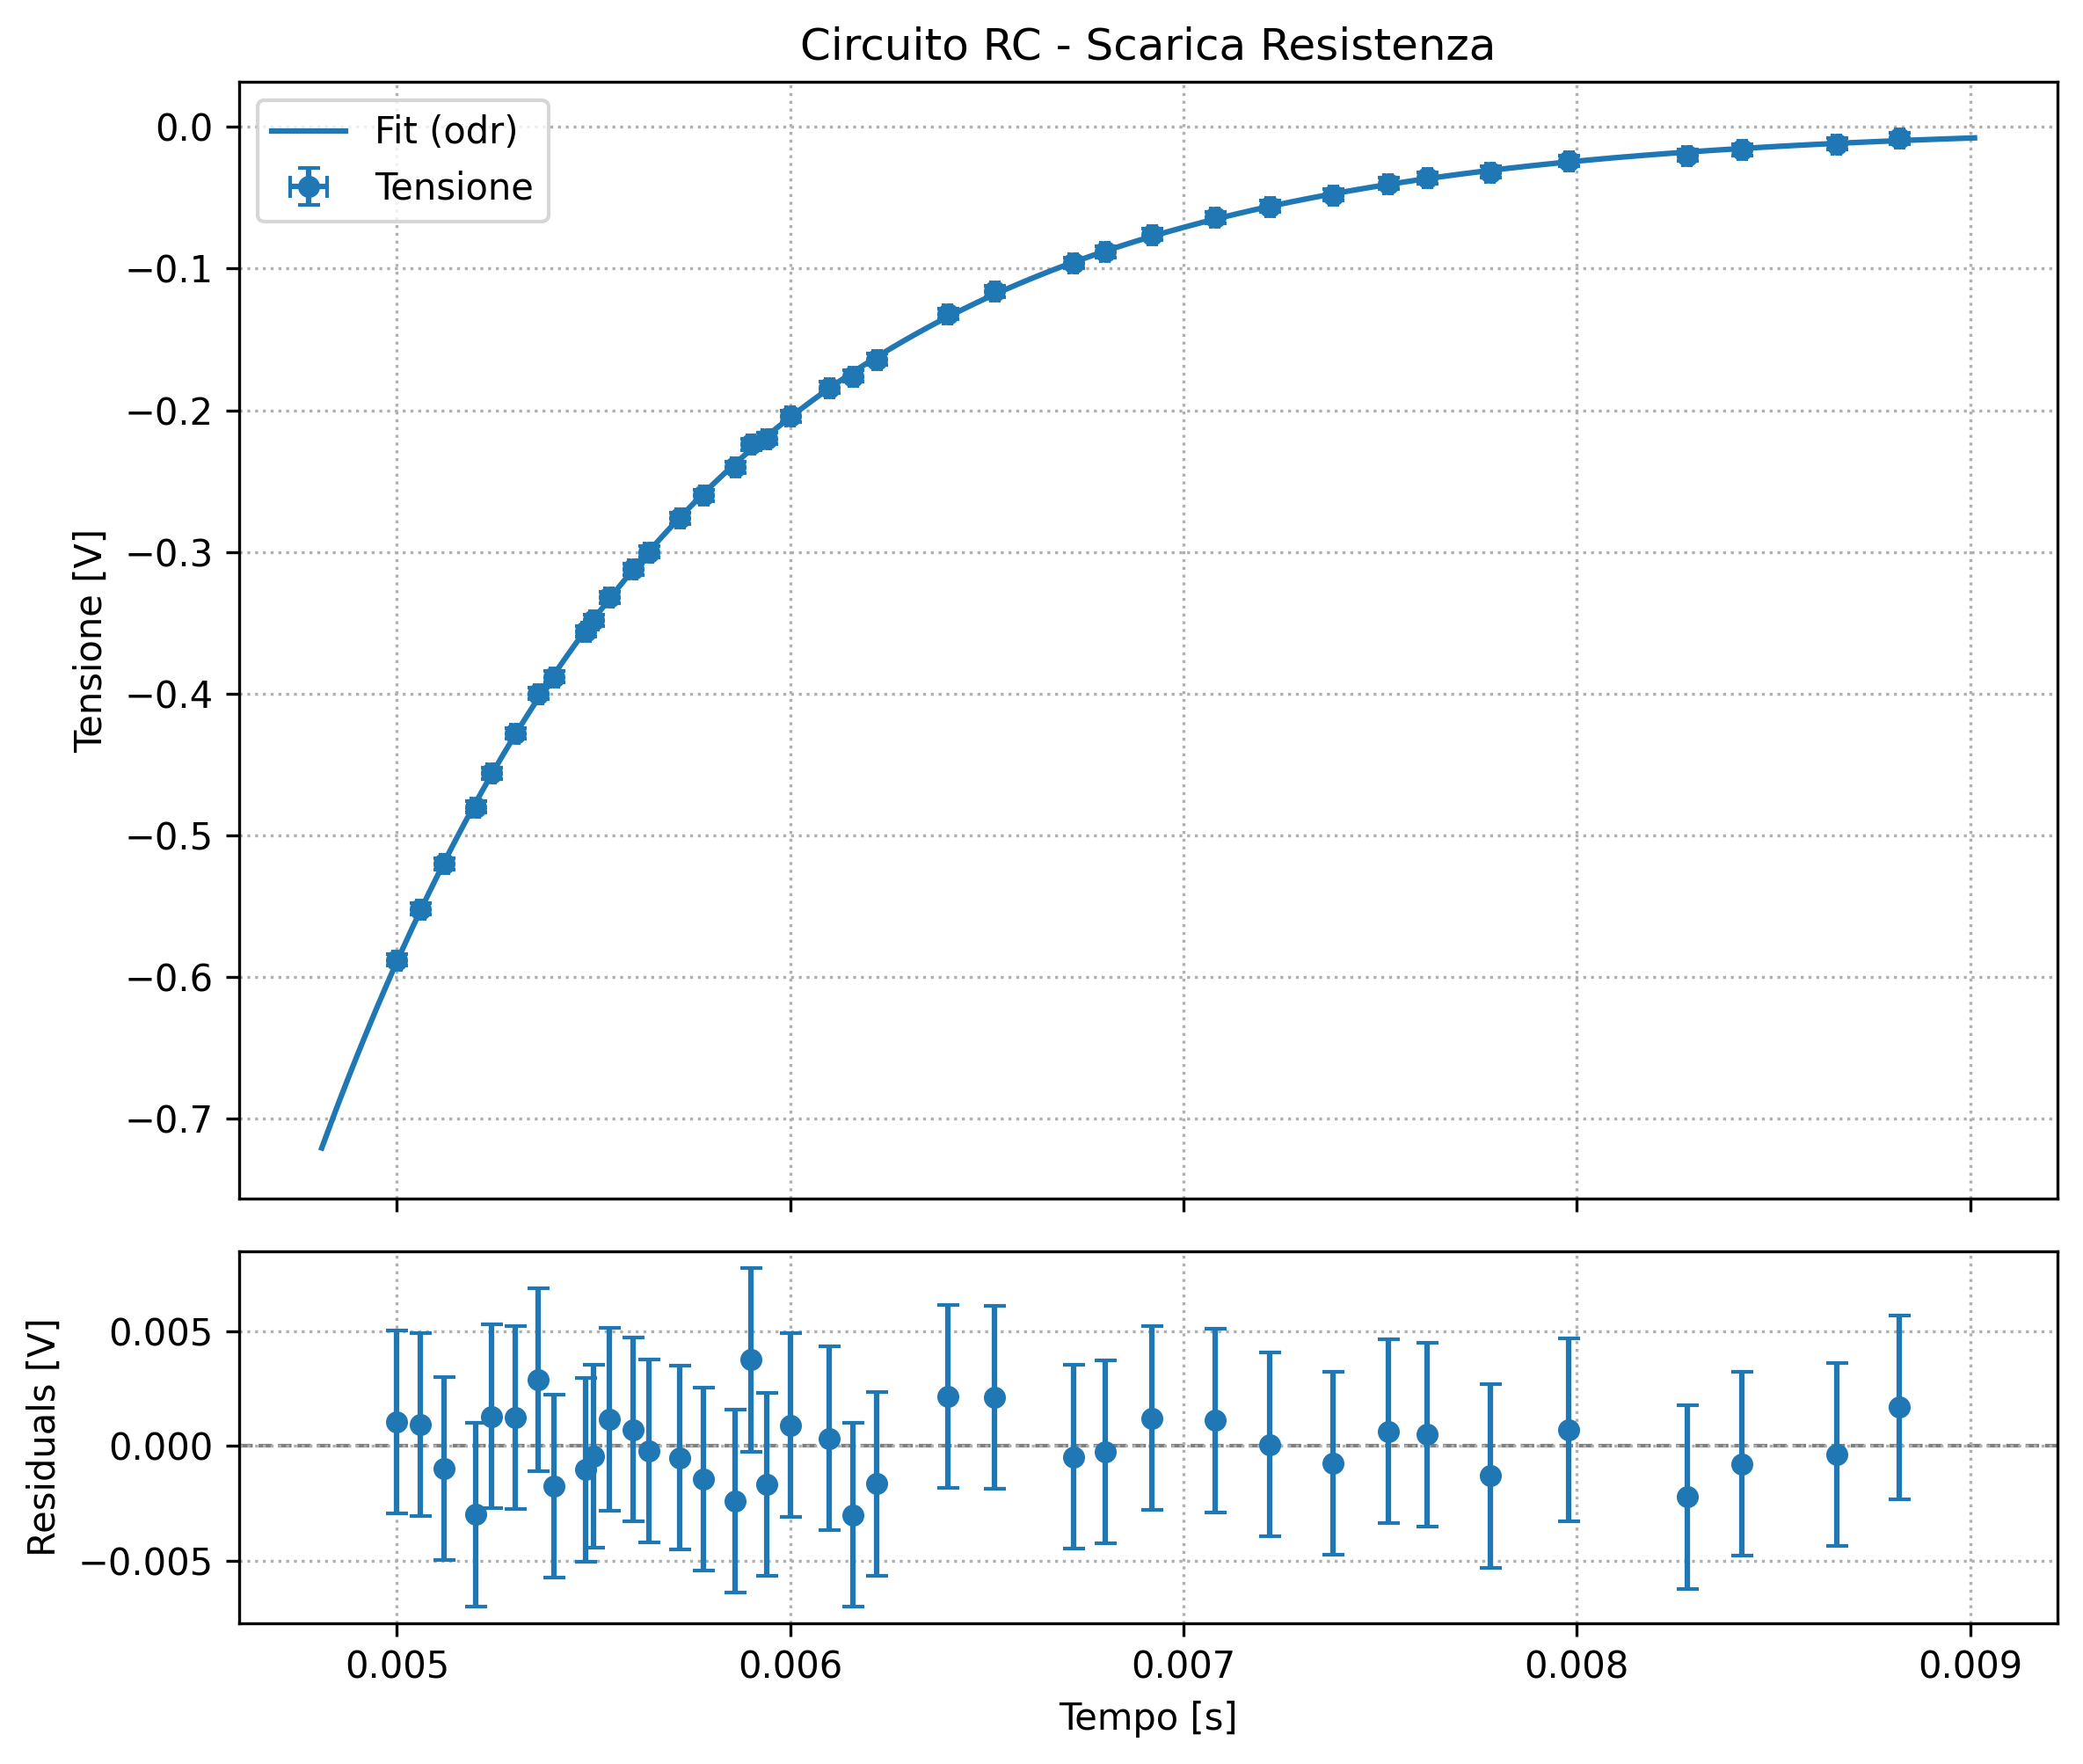
\includegraphics[width=0.9\linewidth]{grafici/rc_scarica_resistenza.png}
    \captionof{figure}{Scarica resistenza - Dati e Fit}
    \label{fig: rc scarica resistenza}
\end{center}

%tabella parametri interpolazione RC (raggruppate)
\begin{table}[htbp]
\centering
\begin{tabular}{|l|cccc|}
\hline
Caso & $\tau$ & $\chi^2$ & DoF & $\chi^2/\nu$ \\ % Cambiata prima colonna
\hline\hline
Scarica Condensatore & 959.6 ± 5.3 µs & 4.22 & 23 & 0.183 \\
Carica Condensatore  & 949.0 ± 3.5 µs & 2.04 & 27 & 0.0754 \\
Carica Resistenza    & 971.0 ± 7.4 µs & 8.53 & 25 & 0.341 \\
Scarica Resistenza   & 949.5 ± 4.2 µs & 4.05 & 35 & 0.116 \\
\hline
\end{tabular}
\caption{Risultati dell'interpolazione per i diversi casi del circuito RC.}
\label{tab:rc_fit_results} % Aggiornato label per distinguerlo se necessario
\end{table}


I valori di $\tau_s$ ricavati sperimentalmente sono stati quindi confrontati con quanto atteso sulla base delle caratteristiche delle componenti del circuito. Abbiamo calcolato $\tau_{att}$ utilizzando la relazione $\tau_{att} = R_{eq}C$, dove $ R_{eq}$ indica la resistenza equivalente, definita così da tener conto della resistenza interna dell'oscilloscopio $R_{osc}$. Essa è stata calcolata utilizzando la relazione $R_{eq}=\frac{RR_{osc}}{R+R_{osc}}$ ed è affetta da errore $\delta_{R_{eq}} = \delta_R(\frac{R_{osc}}{R+R_{osc}})^2$. Ne consegue che l'errore su $\tau_{att}$ può essere determinato utilizzando la formula $\delta_{\tau_{att}}= \sqrt{(\delta_{c}R_{eq})^2 + (\delta_{R_{eq}}C)^2}$.
Quanto utilizzato per determinare $\tau_{att}$ ed il suo valore sono riportati nella Tabella \ref{tab:rc_tau_atteso}.

\begin{table}[htbp] % Era 'center', meglio usare l'ambiente table
\centering
\begin{tabular}{|l|c|}
\hline
C $[\si{nF}]$ & $10.0 \pm 0.1$ \\ % Unità più compatta
\hline
R $[\si{k\ohm}]$ & $100 \pm 1$ \\ % Unità più compatta
\hline
$R_{osc}$ $[\si{M\ohm}]$ & 1\\ % Unità più compatta
\hline
$R_{eq} [\si{k\ohm}]$ & $90.91 \pm 0.9$\\ % Unità più compatta
\hline
$\tau_{att}$ $[\si{ms}]$ & $0.91 \pm 0.09$\\ % Unità più compatta
\hline
\end{tabular}
\caption{Calcolo del valore atteso $\tau_{att}$ per il circuito RC.}
\label{tab:rc_tau_atteso}
\end{table}

I risultati del test di compatibilità tra $\tau_s$ (ottenuto dai fit) e $\tau_{att}$ sono riportati nella Tabella \ref{tab:rc_compatibilita}. Essi derivano dal t-test con \( t = \frac {\tau_s - \tau_{att}}{\sqrt{\delta_{\tau_s}^2+\delta_{\tau_{att}}^2}} \).

\begin{table}[htbp] % Era 'center', meglio usare l'ambiente table
\centering
\begin{tabular}{|l|c|}
\hline
Caso & Probabilità entro t sigma \\
\hline
Scarica condensatore & 0.42 \\
Carica condensatore & 0.34 \\
Scarica resistenza & 0.50 \\
Carica resistenza & 0.34 \\
\hline
\end{tabular}
\caption{Risultati del test di compatibilità tra $\tau_s$ e $\tau_{att}$ per il circuito RC.}
\label{tab:rc_compatibilita}
\end{table}

% Le tabelle di compatibilità erano separate, raggruppate sopra in una sola tabella


Dopodichè considerando noto il valore della parte resistiva del circuito, pari ad $R_{eq}$, abbiamo calcolato il valore di $C$, dalla relazione
 \(C = \frac{\tau_s}{R_{eq}}\) con errore $\delta_c = \sqrt{(\frac{\delta_{\tau_s}}{R_{eq}})^2 + (\delta_{R_{eq}}\frac{\tau_s}{R_{eq}})^2}$.
 Ciò è visualizzabile in Tabella \ref{tab:rc_capacita_ricavate}.

\begin{table}[h!] % Era 'center', meglio usare l'ambiente table
\centering
\begin{tabular}{|l|c|}
\hline
Misura di $\tau_s$ da: & $C_{sperim}$ $[\si{nF}]$ \\ % Unità più compatta
\hline
Scarica condensatore & $10.55 \pm 0.11$  \\
Carica condensatore & $10.44 \pm 0.10$ \\
Scarica resistenza & $10.68 \pm 0.13$ \\
Carica resistenza & $10.44 \pm 0.11$ \\
\hline
\end{tabular}
\caption{Valori di capacità $C$ ricavati dai diversi fit per il circuito RC.}
\label{tab:rc_capacita_ricavate}
\end{table}

Abbiamo infine utilizzato quanto ricavato dal fit (parametri e $\chi^2$ riportati nella Tabella \ref{tab:rc_fit_results}) e i dati sperimentali per effettuare il test del chi quadro. I suoi risultati sono riportati nelle tabelle dei fit stessi.

\subsection{Conclusione}
L'esito del test di compatibilità tra $\tau_s$ e $\tau_{att}$ (Tabella \ref{tab:rc_compatibilita}) dimostra l'accordo di quanto ricavato sperimentalmente con quanto stimato a partire dalle caratteristiche del circuito, una volta che viene attuata la correzione necessaria sulle misure di resistenza (considerando $R_{osc}$). Tale accordo è ritrovato sia valutando l'andamento di $V_c (t)$ che di $V_r (t)$. Anche il test del chi quadro (valori $\chi^2/\nu$ in Tabella \ref{tab:rc_fit_results}) dà esito positivo, dimostrando che le relazioni utilizzate offrono una buona descrizione dell'andamento della tensione ai capi della capacità e della resistenza nel tempo, sia in fase di carica che di scarica.


\section{Circuito RL}
\subsection{Obiettivo}
L'obiettivo di questa esperienza è osservare il comportamento di un circuito composto da una resistenza ed un'induttanza in serie quando esse vengono attraversate da una tensione a onda quadra, verificare se i comportamenti seguiti dal circuito sono concordi alla teoria e misurare il tempo proprio di carica e scarica \( \mathit{\tau} \) e dunque il valore dell'induttanza \( \mathit{L} \).
\subsection{Metodo}
Abbiamo realizzato il circuito $RL$ utilizzando la breadboard, mettendo in serie la resistenza e l'induttanza, sulla base dello schema riportato in figura \ref{fig:rc_circuito} (con $Z = L$ induttanza).  Come generatore abbiamo utilizzato un generatore di tensione fornito dal laboratorio, tramite il quale abbiamo generato un'onda quadra come funzione di tensione, l'offset della funzione era tale da avere un inversione di polarità, da cui abbiamo ricavato gli adamenti attesi. La frequenza di tale onda è stata scelta in modo da poter osservare efficacemente la carica e la scarica del sistema in un tempo ragionevole. Per osservare l'andamento della  tensione all'interno del circuito abbiamo utilizzato un oscilloscopio le cui sonde sono state collegate prima ai capi di \( \mathit{L} \) e del generatore, poi ai capi di \( \mathit{R} \) e del generatore, come era già stato fatto per il circuito RC. Come resistenza abbiamo utilizzato una cassetta delle resistenze, in modo da poter scegliere il valore della resistenza in modo efficace e libero; l'incertezza sul valore delle resistenze date da tale strumento è pari all'\( \mathit{1\%} \) della resistenza scelta. abbiamo scelto un valore di $R$ di $500\si{\ohm}$ con incertezza pari dunque a $5\si{\ohm}$.

%inserire immagini circuiti con sonde su R e L%

Per entrambe le configurazioni abbiamo raccolto almeno 20 misure della coppia di valori \( \mathit{V-t} \) sia per quanto riguarda la carica che la scarica. Per raccogliere tali misure abbiamo utilizzato il cursore sull'interfaccia dell'oscilloscopio campionando \( \mathit{V} \) ad intervalli di tempo arbitrari.
A partire dall'analisi circuitale delle varie configurazioni ci aspettiamo un andamento della tensione di tipo esponenziale. In particolare, ci aspettiamo un andamento di  \( \mathit{V(t)} \) del tipo \footnote{le formule per la scarica sono esattamente queste, mentre per la carica sono invertite di segno}:
\begin{align}
	 & V_L(t) = \frac{2V_g}{1+e^-\frac{T}{\mathit{2\tau}}}e^{-\frac{t}{\mathit{\tau}}}  \quad \text{e} \quad V_R(t) = V_g\left(1-\frac{2e^-\frac{t}{\mathit{\tau}}}{1+e^-\frac{T}{\mathit{2\tau}}}\right)\quad \label{eq:rl_full} % Cambiato label
\end{align}
Nelle formule \( \mathit{V_L(t)} \) è la tensione misurata ai capi dell'induttanza, \( \mathit{V_R(t)} \)  è la tensione misurata ai capi della resistenza, \( \mathit{V_g} \) è la tensione erogata dal generatore, \( \mathit{T} \)  è il periodo dell'onda quadra e \( \mathit{\tau=\cfrac{L}{R}} \)  con \( \mathit{L} \) valore dell'induttanza e \( \mathit{R} \) valore della resistenza. Il valore del periodo \( \mathit{T} \) dell'onda quadra è arbitrario e può essere regolato direttamente dal generatore di tensione. Per poter osservare una scarica ed una carica completa abbiamo scelto un valore del periodo tale che \( \mathit{T\approx10\mathit{\tau}} \) , dunque possiamo affermare che \( \mathit{e^-\frac{T}{2\tau}}\approx 0 \) , dunque tali formule possono essere riscritte in maniera più compatta come: \begin{align}
	 & V_L(t) = 2V_ge^{-\frac{t}{\mathit{\tau}}}  \quad \text{e} \quad V_R(t) = V_g(1-2e^{-\frac{t}{\mathit{\tau}}})\quad \label{eq:rl_approx} % Cambiato label
\end{align}
con un fattore di bias di  $1-\frac{1}{1+e^{-5}}=0,007$ che è trascurabile perchè inferiore agli errori relativi.

\subsection{Dati}
Di seguito portiamo i riferimenti alle tabelle contenenti i dati raccolti durante l'esperimento mediante l'oscilloscopio, che si trovano in Appendice \ref{app:dati_rl}.
Nelle Tabelle \ref{tab:rl_data_scarica_l} e \ref{tab:rl_data_carica_l} sono indicati i dati dell'intervallo di tempo e voltaggio durante la scarica e la carica ai capi dell'induttore.
Nelle Tabelle \ref{tab:rl_data_scarica_r} e \ref{tab:rl_data_carica_r} sono indicati i valori dei dati dell'intervallo di tempo e voltaggio durante la carica e scarica ai capi della resistenza.
Come errori abbiamo considerato la sensibilità dell'oscilloscopio, dunque un errore uniforme di \( 0,01 ms \) (o \( 10 \, \mu s \)) per i tempi ed un errore di \( 0,02mV \) (o \( 2 \, mV \)) sulle tensioni.
Da notare è il fatto che gli intervalli di tempo e voltaggio sono presi in maniera relativa ad un valore iniziale, infatti nè il tempo nè il voltaggio partono necessariamente da \( \mathit{0} \) come indicato nelle formule attese. Ciò è da imputare al fatto che la funzione di carica e scarica fosse traslata rispetto all'origine degli assi sull'oscilloscopio. Tuttavia ciò che è importante ai fini del nostro esperimento sono i valori relativi, infatti per avere la curva di carica e scarica attesa basterà traslare i dati ottenuti in tabella (e dunque traslare la funzione interpolata) di un fattore pari al pimo tempo e al primo voltaggio.

% Le tabelle dati RL sono state spostate in appendice

\subsection{Analisi Dati}
Considerando le misure effettuate in laboratorio (riportate in Appendice \ref{app:dati_rl}) abbiamo fittato i dati secondo la legge attesa per ciascuna configurazione (Eq. \ref{eq:rl_approx}, tenendo conto delle traslazioni $V_0, t_0$). Per quanto riguarda la carica e scarica ai capi dell'induttore avremo una legge del tipo \( \mathit{V_L(t) = k \cdot e^{-\frac{(t-t_0)}{\mathit{\tau}}} + c}\) (o simile, a seconda dell'implementazione del fit), dove $\tau$ è il parametro di interesse. Per la resistenza avremo una forma analoga ma basata sulla formula per $V_R(t)$.
\begin{center}
    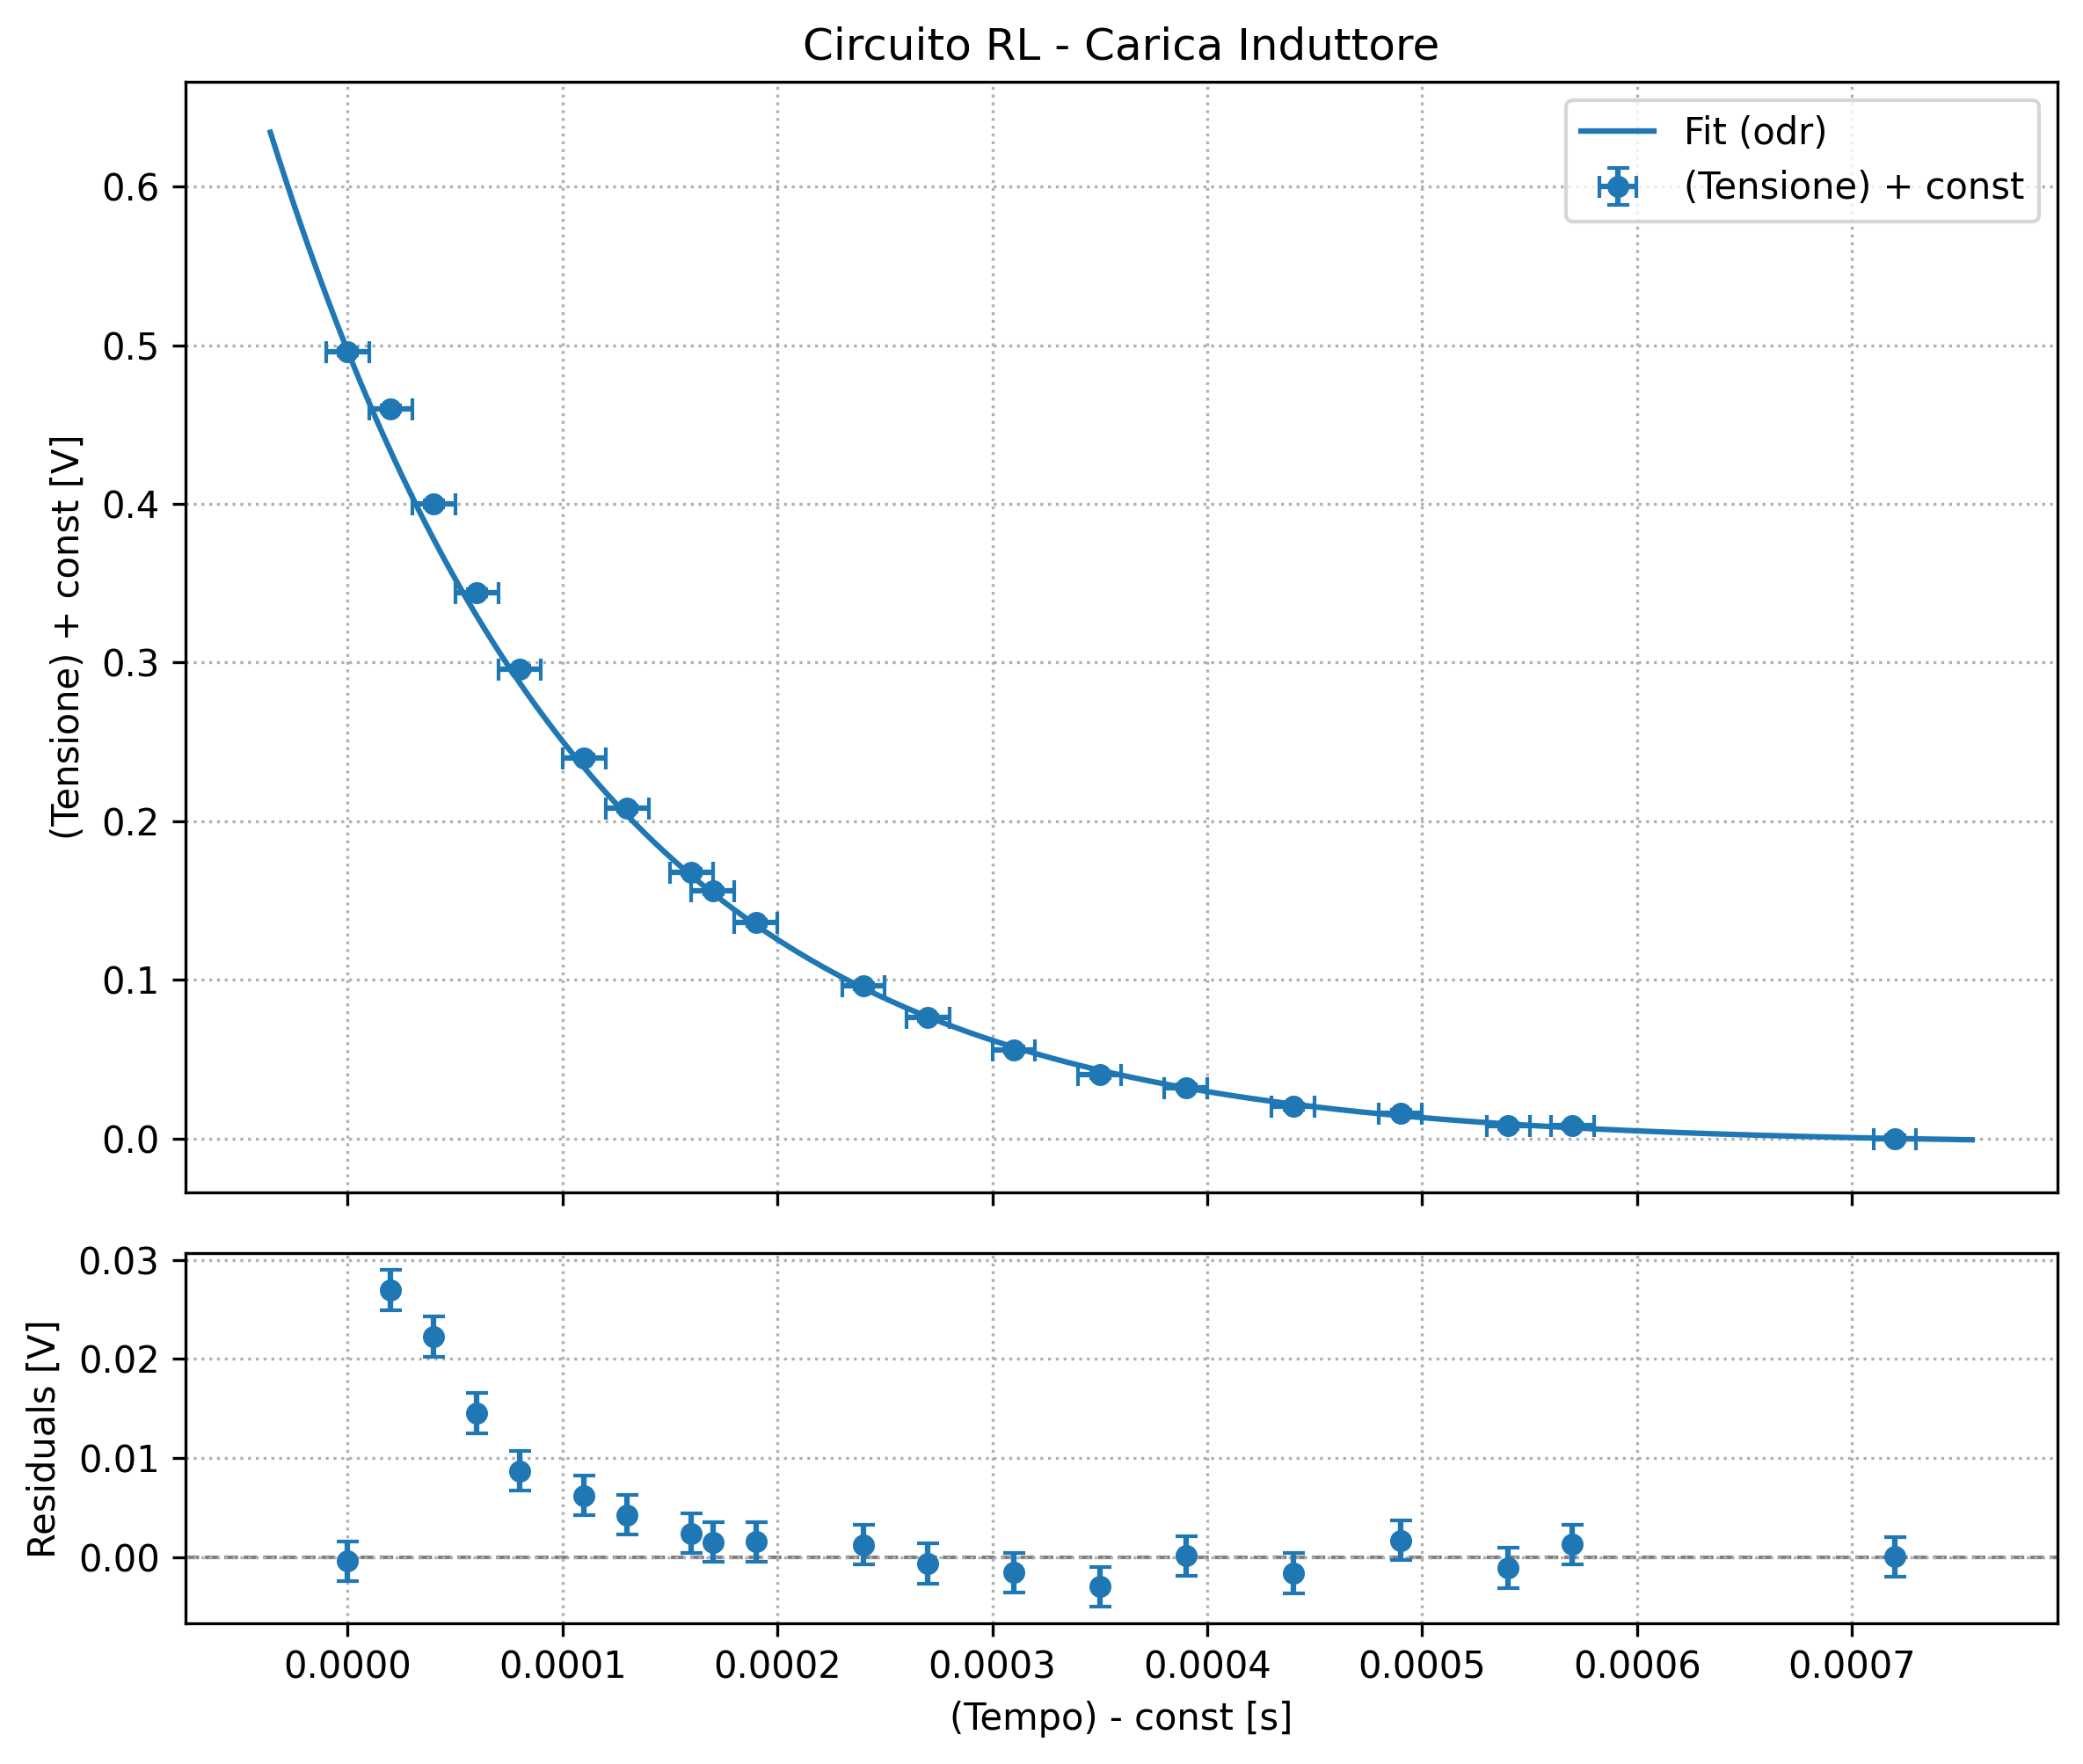
\includegraphics[width=0.9\linewidth]{grafici/rl_carica_induttore.png}
    \captionof{figure}{Carica induttore - Dati e Fit}
    \label{fig: rl carica induttore}
    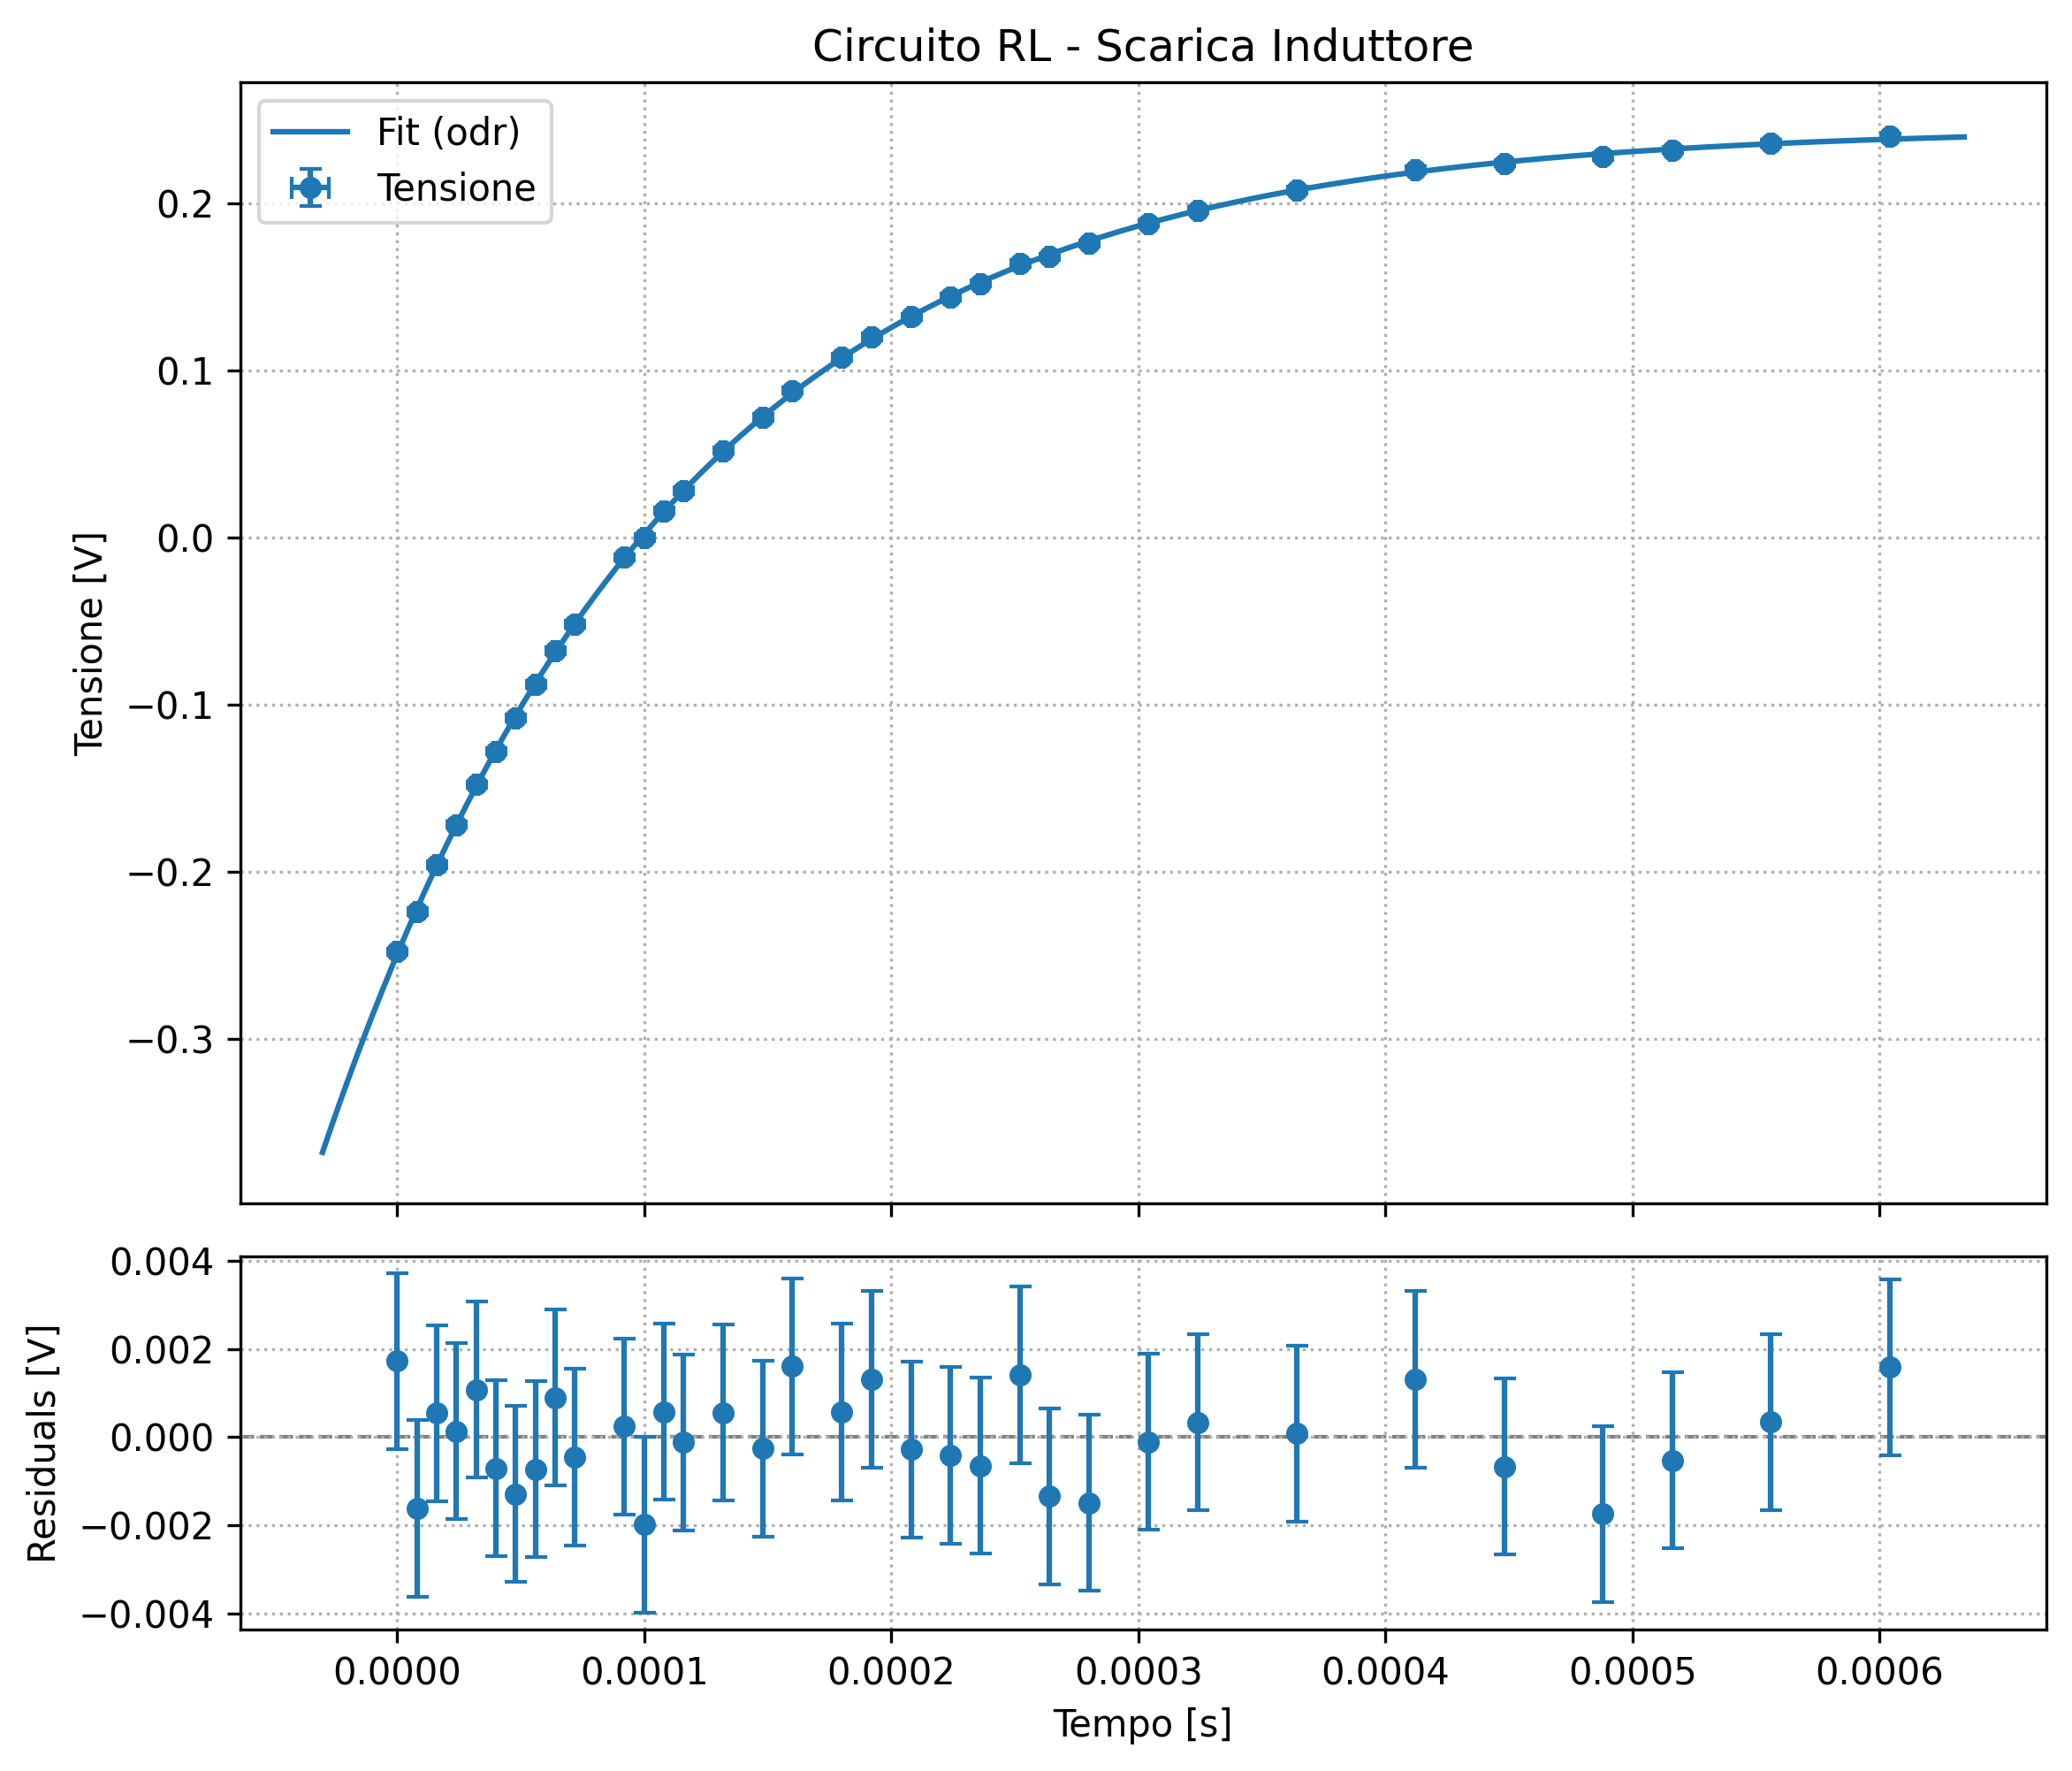
\includegraphics[width=0.9\linewidth]{grafici/rl_scarica_induttore.png}
    \captionof{figure}{Scarica induttore - Dati e Fit}
    \label{fig: rl scarica induttore}
    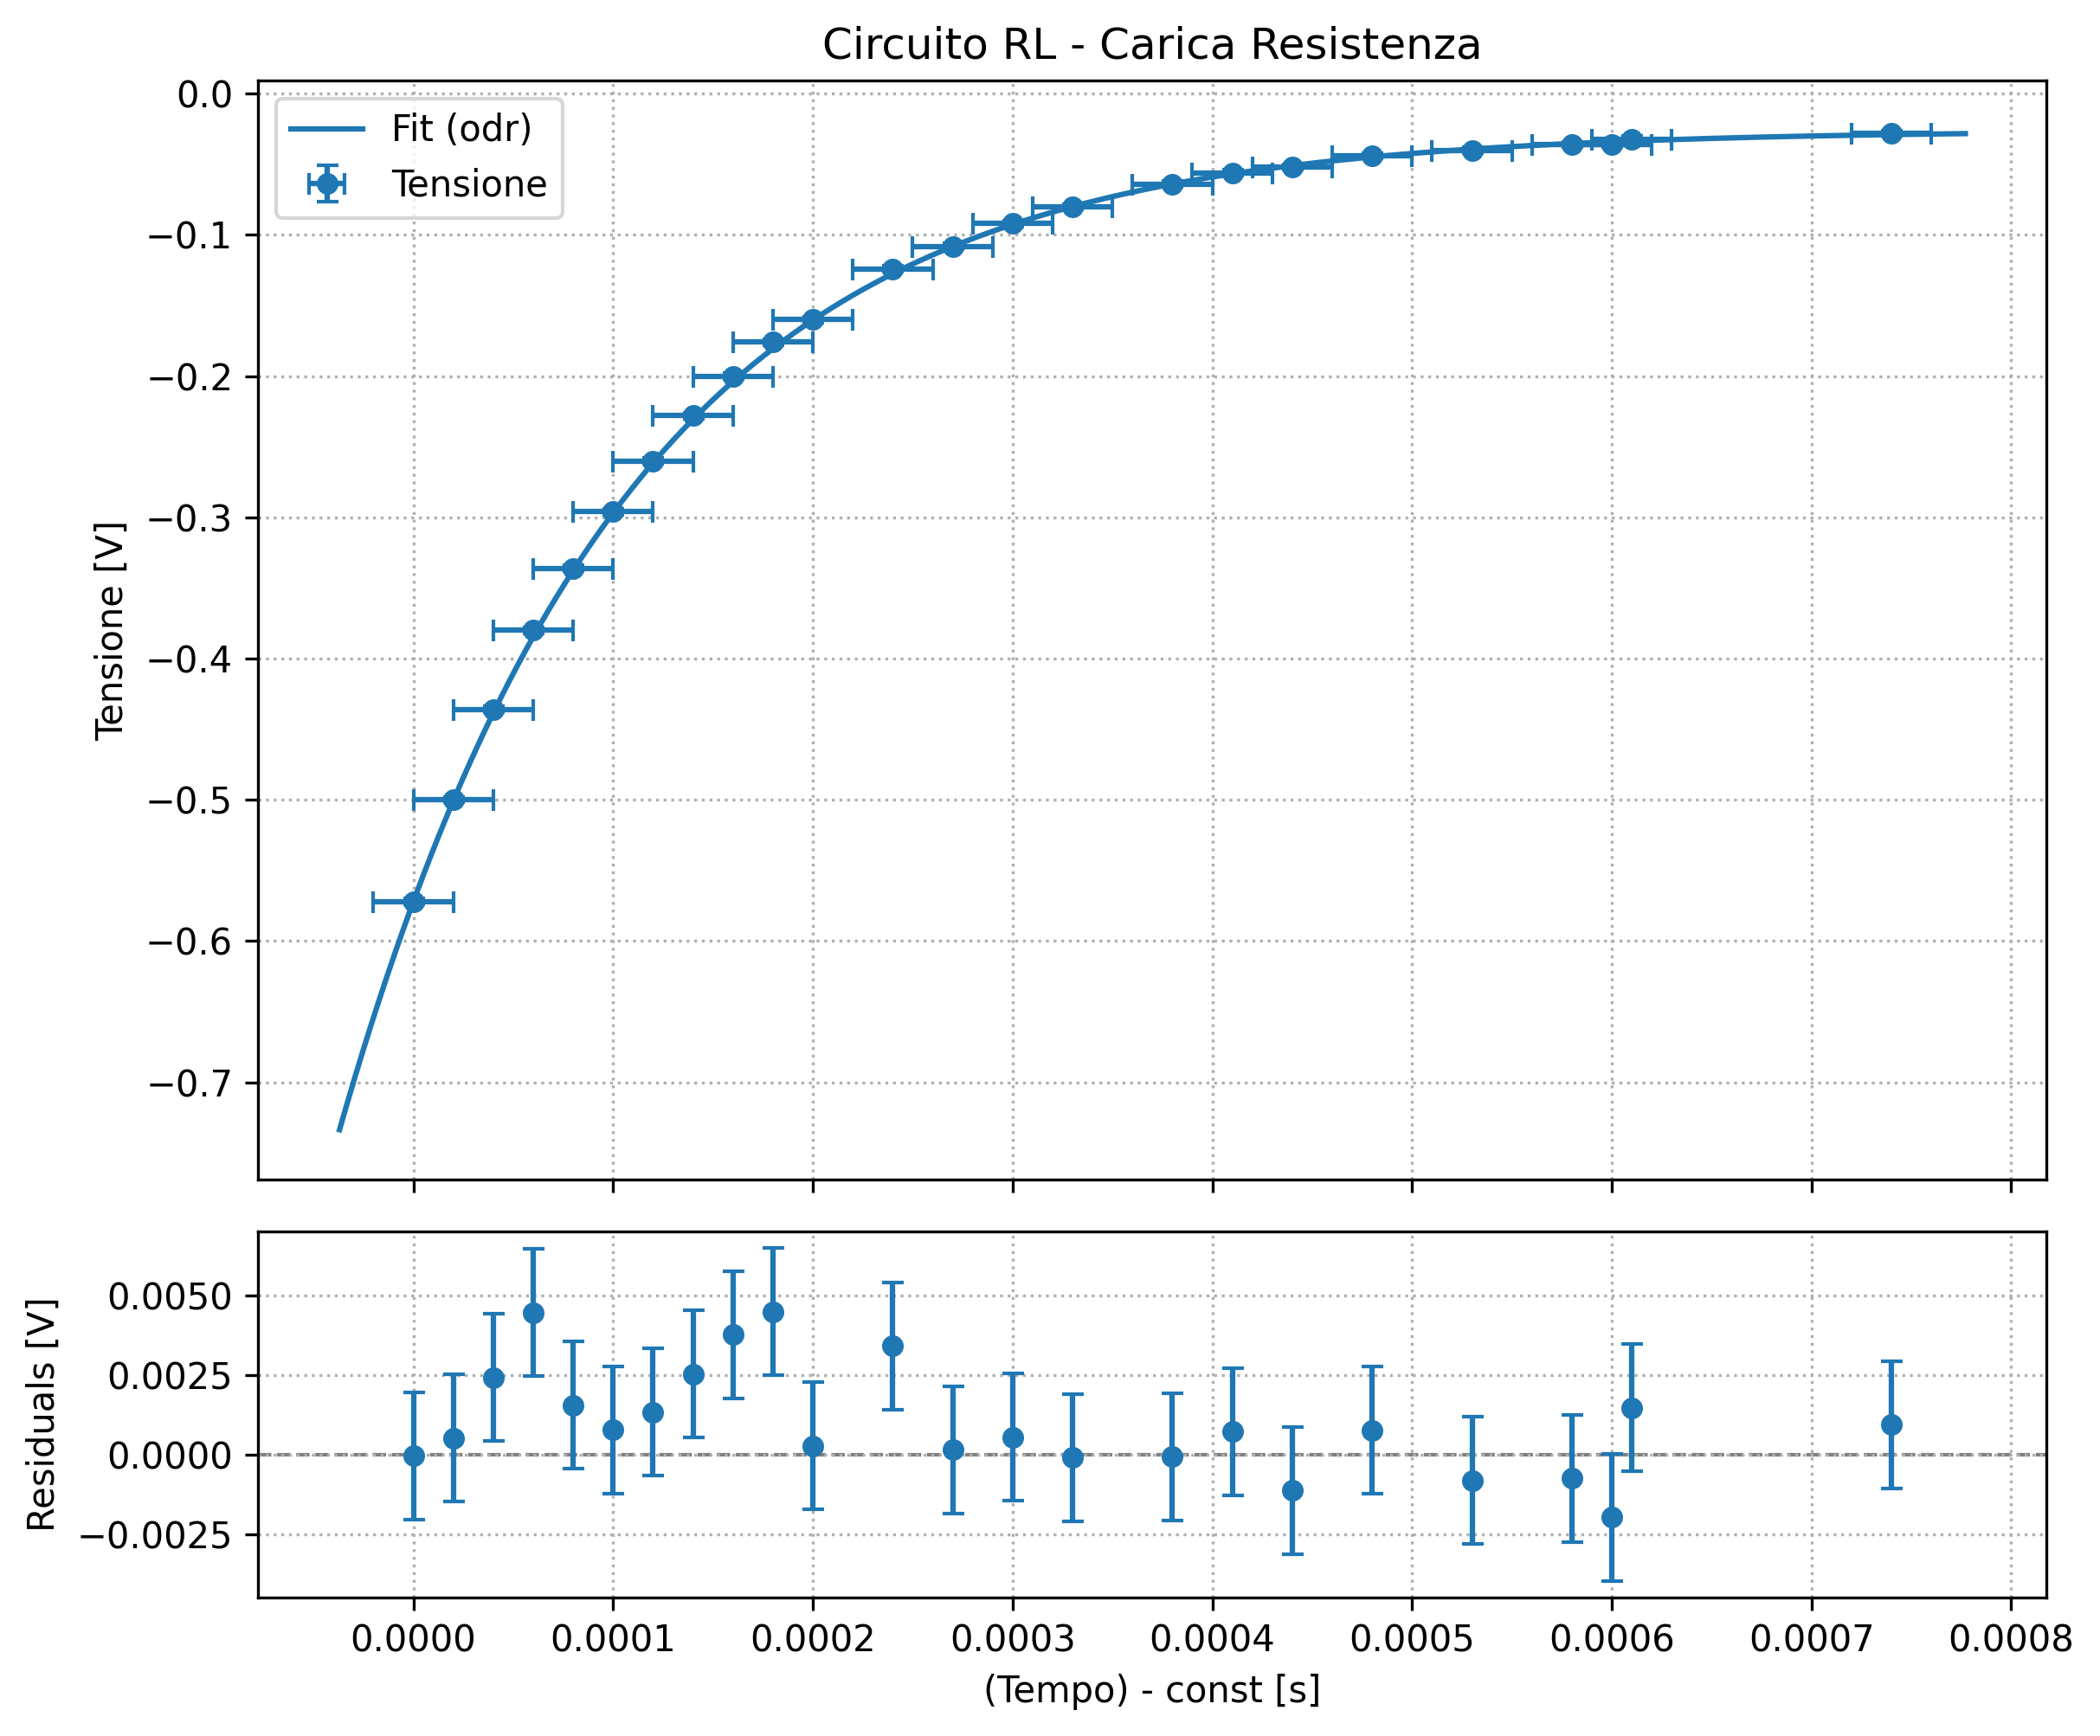
\includegraphics[width=0.9\linewidth]{grafici/rl_carica_resistenza.png}
    \captionof{figure}{Carica resistenza - Dati e Fit}
    \label{fig: rl carica resistenza}
    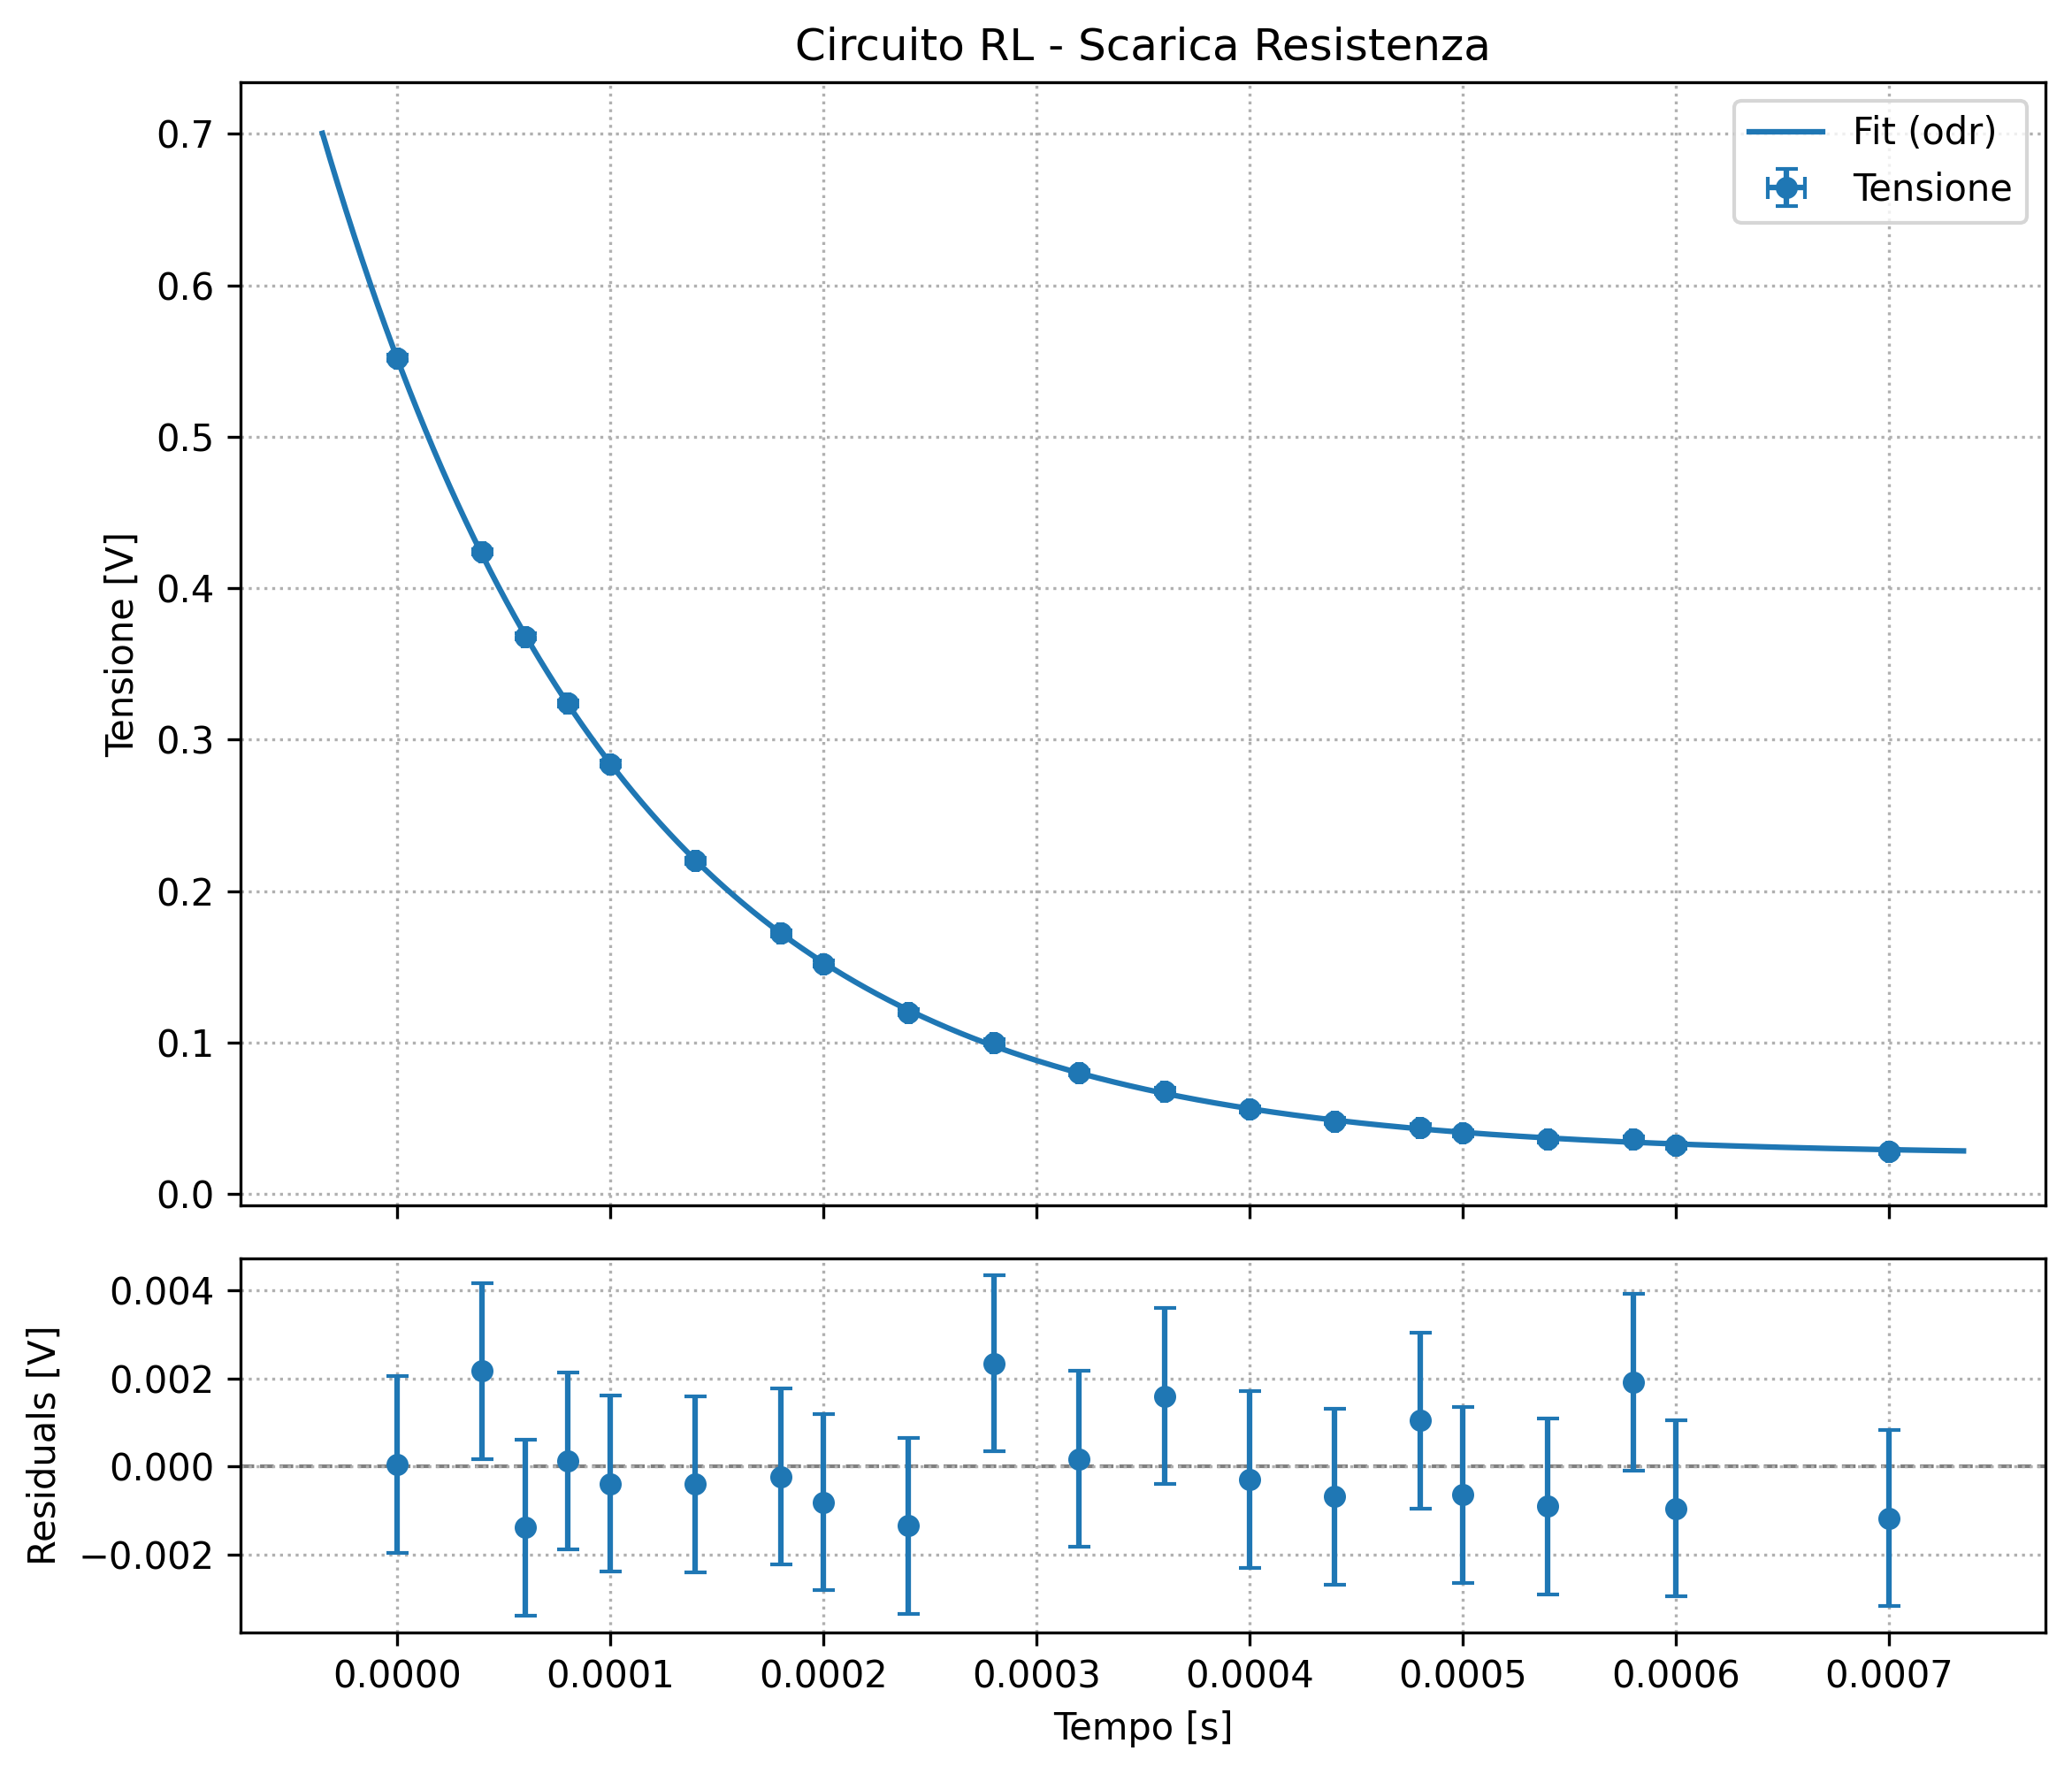
\includegraphics[width=0.9\linewidth]{grafici/rl_scarica_resistenza.png}
    \captionof{figure}{Scarica resistenza - Dati e Fit}
    \label{fig: rl scarica resistenza}
\end{center}
%inserire interpolazione e considerazioni%
% I grafici di interpolazione per RL non erano presenti nel documento originale.
% Se disponibili, andrebbero inseriti qui come per RC.

Consideriamo ora il valore della resistenza. Come anticipato nella sezione precedente la resistenza della cassetta $R$ è stata scelta in maniera arbitraria ed il suo valore è di $(500\pm5)\si{\ohm}$. Tuttavia il valore della resistenza totale viene influenzato anche dalle resistenze interne del generatore e dell'oscilloscopio. La resistenza interna del generatore di tensione $R_g$ è molto bassa, dell'ordine di $1\si{\ohm}$, e tale resistenza è in serie con $R$; il bias dovuto a ciò sarà dunque trascurabile poichè l'incertezza sul valore di $R$ è maggiore del valore di $R_g$. La resistenza interna dell'oscilloscopio $R_\textbf{osc}$ è invece di circa $1M\si{\ohm}$; la resistenza equivalente $R_{\textbf{eq}}$ sarà dunque $R_{eq}=\frac{RR_{osc}}{R+R_{osc}}=499,8\si{\ohm}$. Tale valore crea un bias di $0,2\si{\ohm}$ che è molto inferiore all'incertezza sulla resistenza. I bias dovuti alle resistenze degli strumenti sono dunque trascurabili. Useremo quindi $R_{eq} \approx R = (500 \pm 5)\si{\ohm}$ per i calcoli successivi.


Dall'interpolazione dei dati (i cui risultati sono mostrati in Tabella \ref{tab:rl_fit_results}) si ottengono i valori di $\tau_s$.

%tabella parametri interpolazione RL (raggruppate)
\begin{table}[htbp]
\centering
\begin{tabular}{|l|cccc|} % Ridotto il numero di colonne a lcccc (Caso + 4 valori)
\hline
Caso & $\tau$ [\si{\micro s}] & $\chi^2$ & DoF & $\chi^2/\nu$ \\ % Intestazione aggiornata, unità per tau
\hline\hline
Scarica Induttore & 140.75 ± 0.50 & 6.06 & 31 & 0.196 \\
Carica Induttore  & 147.8 ± 1.6   & 4.75 & 17 & 0.279 \\
Scarica Resistenza& 140.89 ± 0.78 & 5.31 & 17 & 0.312 \\
Carica Resistenza & 142.6 ± 1.2   & 1.85 & 21 & 0.0882 \\
\hline
\end{tabular}
\caption{Risultati dell'interpolazione per i diversi casi del circuito RL.}
\label{tab:rl_fit_results}
\end{table}


% La tabella singola con tau e L è stata rimossa perché ridondante con le tabelle dei fit e la tabella delle induttanze calcolate sotto.
-+

Dopodichè considerando noto il valore della parte resistiva del circuito, $R = (500 \pm 5)\si{\ohm}$, abbiamo calcolato il valore di $L$ da ciascun fit, usando la relazione \(L = \tau_s R\) con errore $\delta_L = \sqrt{(\delta_{\tau_s}R)^2 + (\delta_{R}\tau_s)^2}$. Ciò è visualizzabile in Tabella \ref{tab:rl_induttanze_ricavate}.

\begin{table}[htbp] % Era 'center', meglio usare l'ambiente table
\centering
\begin{tabular}{|l|c|}
\hline
Misura da: & $L_{sperim}$ $[\si{mH}]$ \\ % Unità più compatta
\hline
Scarica induttore & $70.4 \pm 0.7$  \\ % (140.75e-6 * 500 = 0.070375)
Carica induttore  & $73.9 \pm 0.9$ \\ % (147.8e-6 * 500 = 0.0739)
Scarica resistenza & $70.4 \pm 0.8$ \\ % (140.89e-6 * 500 = 0.070445)
Carica resistenza & $71.3 \pm 0.9$ \\ % (142.6e-6 * 500 = 0.0713) % ATTENZIONE: Unità errata nell'originale (10^-9)
\hline
\end{tabular}
\caption{Valori di induttanza $L$ ricavati dai diversi fit per il circuito RL.}
\label{tab:rl_induttanze_ricavate}
\end{table}

I parametri ricavati dal fit e i dati sperimentali sono infine stati utilizzati per effettuare il test del chi quadro, i cui risultati ($\chi^2/\nu$) sono riportati nella Tabella \ref{tab:rl_fit_results}.


\subsection{Conclusioni}
Alla luce dei dati ottenuti e degli esiti positivi dei test del chi quadro (valori di $\chi^2/\nu$ nella Tabella \ref{tab:rl_fit_results}, tutti $\ll 1$), possiamo affermare che la legge attesa (Eq. \ref{eq:rl_approx}) è verificata per l'andamento della tensione sia ai capi dell'induttore che della resistenza. Inoltre, abbiamo ricavato il valore di $L$, non noto, dai diversi fit, come mostrato in tabella \ref{tab:rl_induttanze_ricavate}, e abbiamo stimato $L \approx (71.5 \pm 0.5) \, \si{mH}$ tramite la media pesata.


\section{Circuito RLC}
\subsection{Obiettivo}
Studiare l'andamento della differenza di potenziale nel tempo ai capi della resistenza inserita in un circuito RLC, alimentato da un generatore di tensione impostato su segnale ad onda quadra.

\subsection{Metodo}
\begin{center}
	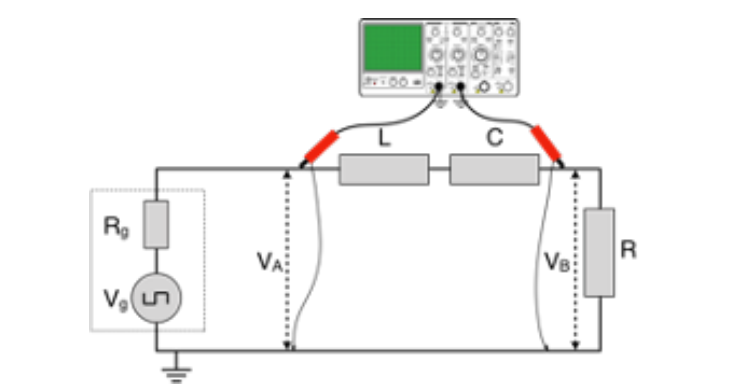
\includegraphics[width=0.5\textwidth]{grafici/circuito-rlc.png}
	\captionof{figure}{Circuito RLC}
	\label{fig:rlc_circuito} % Cambiato label
\end{center}
Innanzitutto abbiamo ricostruito il circuito rappresentato schematicamente in figura \ref{fig:rlc_circuito}; per farlo abbiamo collegato in serie condensatore, induttore e resistore, scegliendo la cassetta di resistenze per poter variare più agevolmente il valore di $R$. Abbiamo quindi utilizzato l'oscilloscopio per visualizzare l'andamento della tensione. Mediante l'insimento di due sonde, l'una in parallelo con il generatore, e l'altra in parallelo con la resistenza, abbiamo infatti potuto osservare il segnale di $V_g$, tensione fornita dal generatore, confermando che essa avesse un andamento quadro, e di $V_R$. Abbiamo quindi campionato la forma di $V_R$ utilizzando i cursori dell'oscilloscopio, tramite cui abbiamo ricavato il valore della coppia $V_R-t$ al variare del tempo $t$. Tale processo è stato ripetuto in regime sottosmorzato, sovrasmorzato e di smorzamento critico. A partire dall'analisi circuitale e dalle relazioni caratteristiche per ciascun componente, è stato possibile dedurre le condizioni per cui si instaura un determinato regime. Definiti:
\begin{align}
	 & \gamma = \frac {R}{2L} \quad \text{e} \quad \omega_0 = \frac {1}{\sqrt{LC}} \label{eq:rlc_params} % Cambiato label
\end{align}
con $R$ resistenza interna al circuito, $L$ induttanza e $C$ capacità del condensatore, è possibile stimarne la relazione e il conseguente regime .
In particolare si può ricavare:
\begin{itemize}
	\item \( \mathit{\gamma < \omega_0} \): regime sottosmorzato
	\item \( \mathit{\gamma > \omega_0} \): regime sovrasmorzato
	\item \( \mathit{\gamma = \omega_0} \): regime di smorzamento critico ($\gamma \simeq \omega_0$ in pratica)
\end{itemize}
Per studiare quindi il funzionamento del circuito in tutte e tre i regimi abbiamo dovuto modificarne le caratteristiche, più nello specifico abbiamo scelto di agire sul valore di $R$, al fine di variare la relazione tra \( \mathit{\gamma}\) e \( \mathit{\omega_0}\) I valori di resistenza tali per cui è stato possibile effettuare questo processo sono riportati in Tabella \ref{tab:rlc_resistenze}. Essi sono stati scelti valutando la forma d'onda resistituita dall'oscilloscopio al variare di $R$.
\begin{table}[htbp] % Era 'center', meglio usare l'ambiente table
\centering
\begin{tabular}{|l|c|}
\hline
Regime & R $[\si{\ohm}]$ \\
\hline
Sottosmorzato & $500 \pm 5$\\
Sovrasmorzato & $15000 \pm 150$ \\ % Riscritto come numero
Smorzamento critico & $5300 \pm 53$ \\ % Riscritto come numero
\hline
\end{tabular}
\caption{Valori della resistenza $R$ utilizzati per i diversi regimi del circuito RLC.}
\label{tab:rlc_resistenze}
\end{table}

\subsection{Dati}
Nelle Tabelle \ref{tab:rlc_data_sottosmorzato}, \ref{tab:rlc_data_sovrasmorzato} e \ref{tab:rlc_data_critico} (riportate in Appendice \ref{app:dati_rlc}) sono raccolti i valori di tensione ai capi della resistenza e tempo per ciascun regime. Per il regime sovrasmorzato e di smorzamento critico abbiamo raccolto circa 35 valori della coppia $V_R-t$, mentre per il regime di sottosmorzamento abbiamo raccolto 52 valori di $V_R-t$, al fine di poter meglio campionare la forma d'onda.
Per la stima dell'errore abbiamo considerato la sensibilità degli strumenti di misura, cioè la precisione associata alle misure di tensione e tempo ricavate spostando il cursore lungo la curva $V_R(t)$ mostrata dall'oscilloscopio.

% Le tabelle dati RLC sono state spostate in appendice

\subsection{Analisi dati}
Abbiamo poi interpolato i dati raccolti utilizzando per ciascun regime la legge caratteristica, come visibile all'interno dei grafici \ref{fig: rlc sottosmorzato}, \ref{fig: rlc sovrasmorzato} e \ref{fig: rlc critico}.
\begin{itemize}
	\item regime sottosmorzato : \(V_R(t) = V_0 e^{-\gamma t }\sin (\beta t)\)
	\item regime sovrasmorzato : \(V_R(t) = V_0 e^{-\gamma t } (e^{\beta t} - e^{-\beta t}) \)
	\item regime di smorzamento critico : \(V_R(t) = V_0 t e^{-\gamma t } \)
\end{itemize}
Riportiamo nella Tabella \ref{tab:rlc_fit_results} i valori delle costanti caratteristiche del circuito stimate in ciascuna configurazione e i rispettivi errori, ccome ottenuto dal fit.

%grafici (da inserire se disponibili)
\begin{center}
    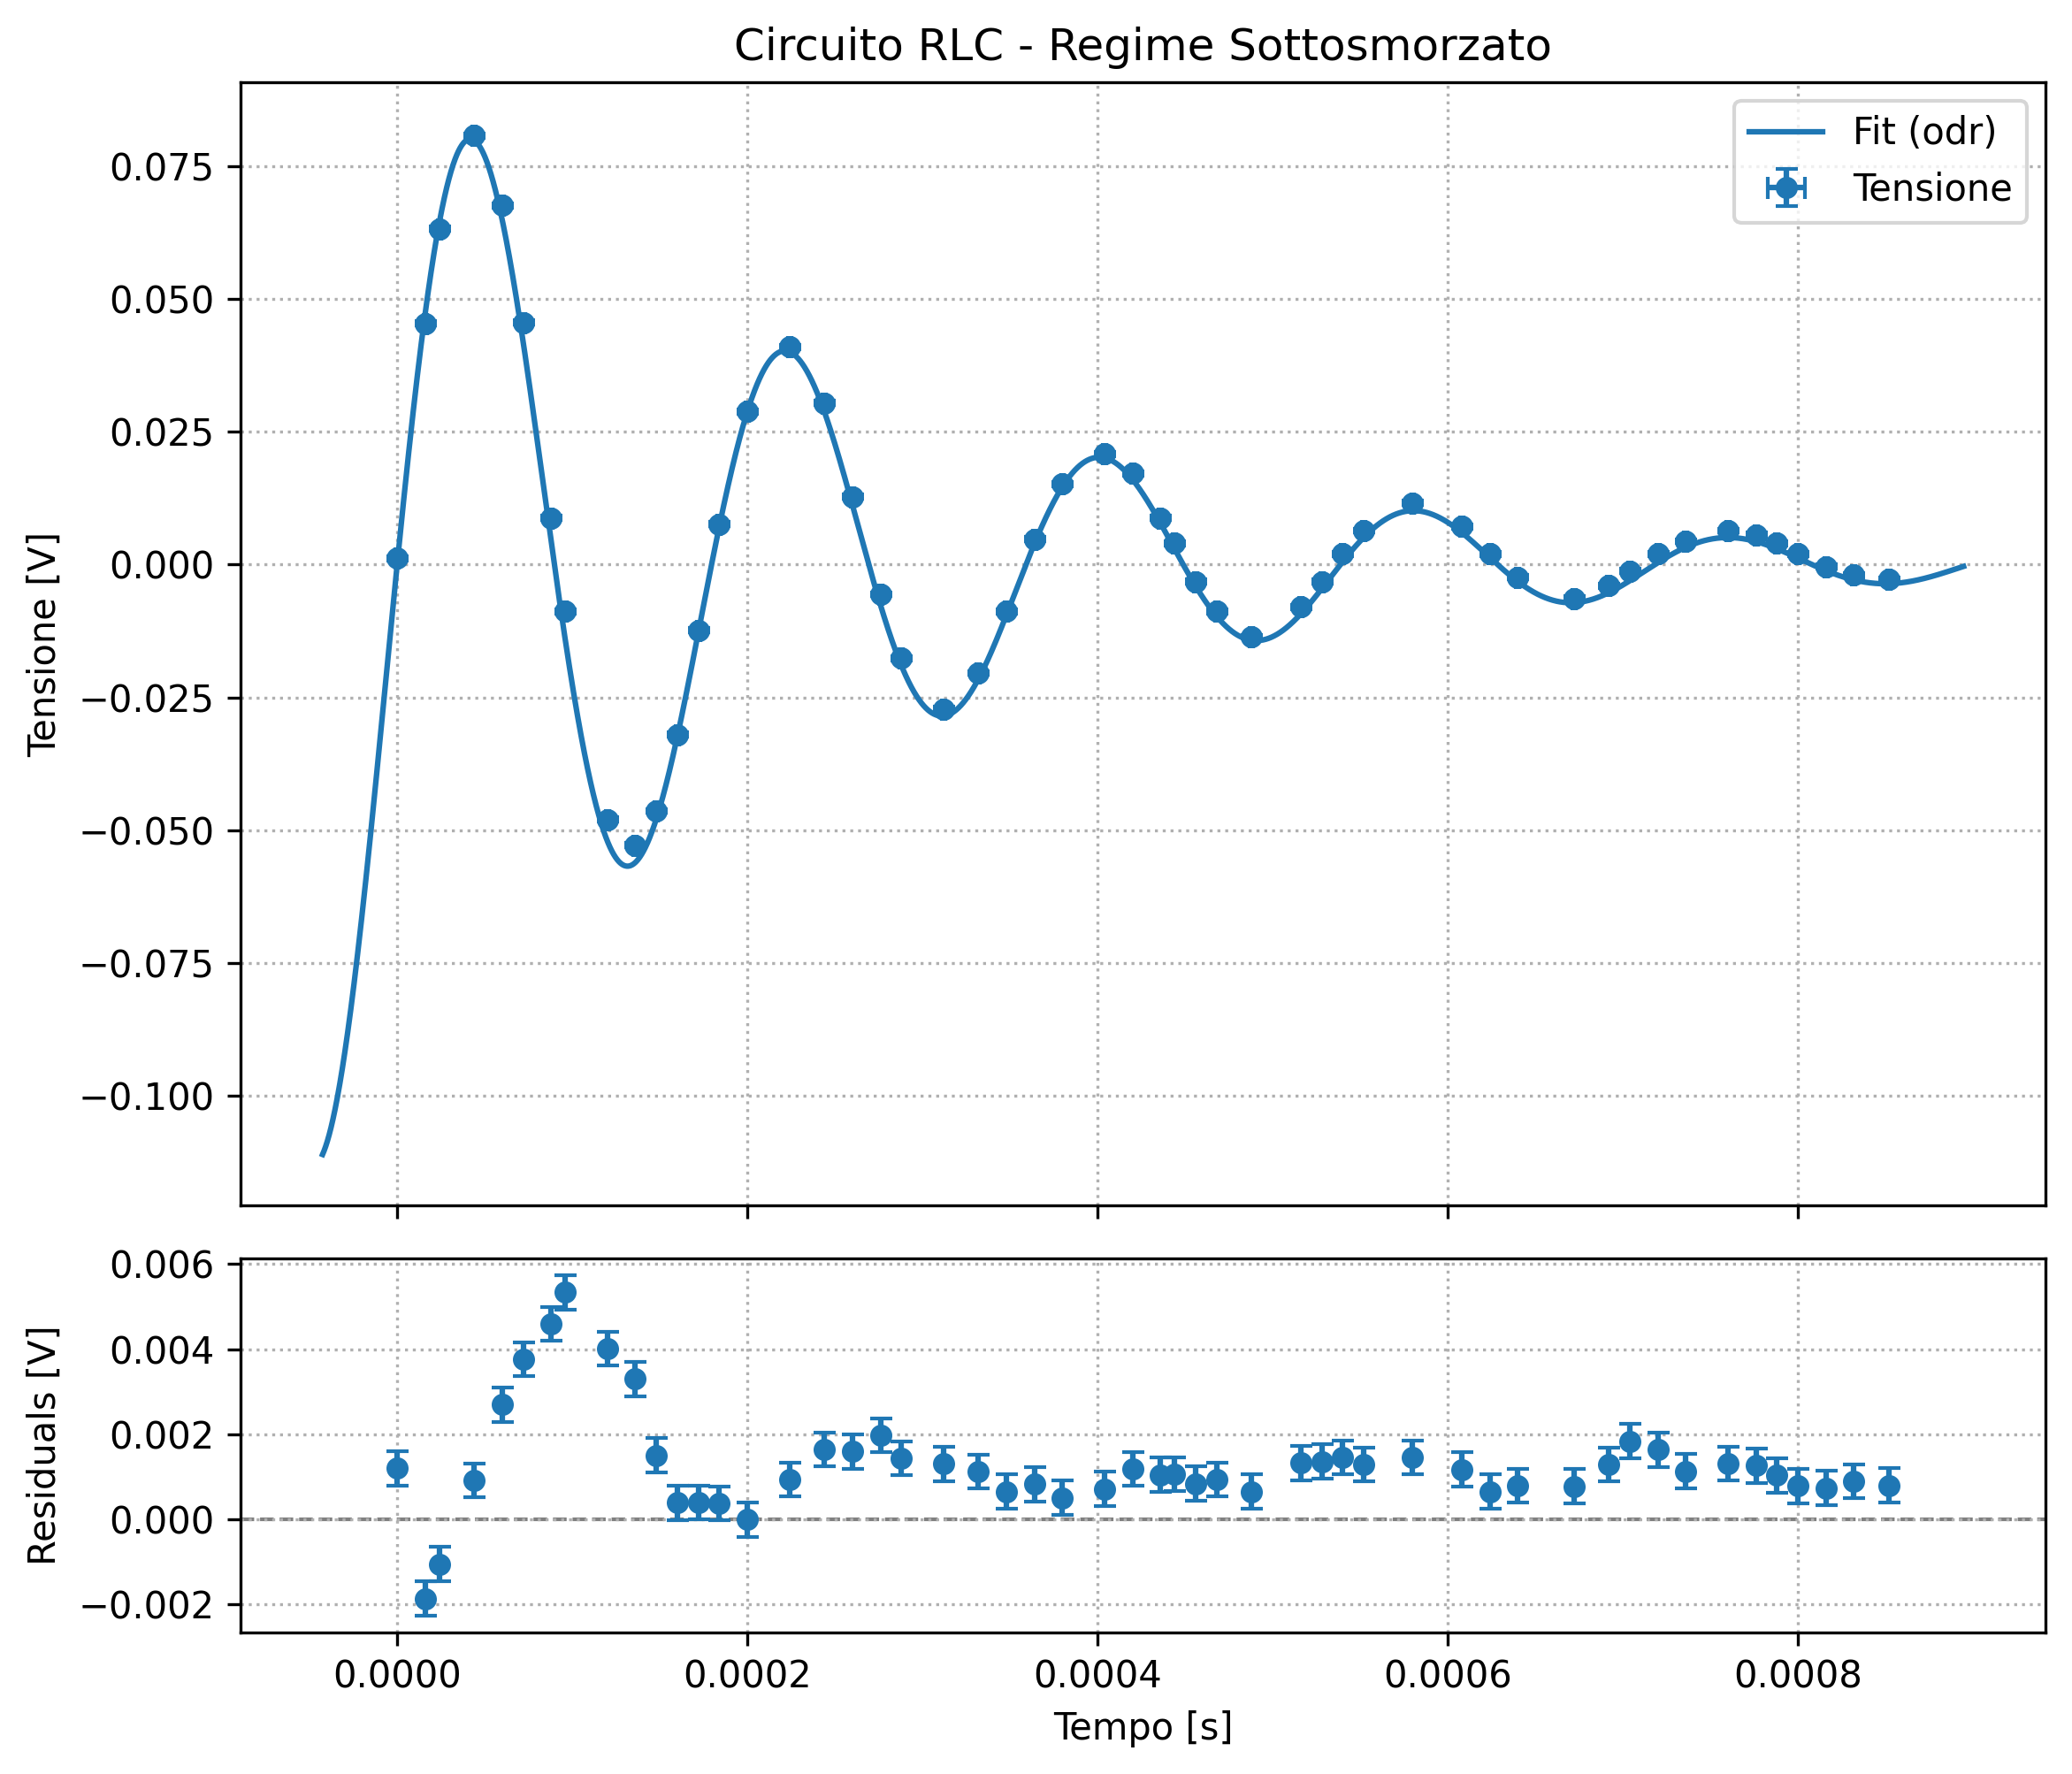
\includegraphics[width=0.9\linewidth]{grafici/sottosmorzato.png}
    \captionof{figure}{Regime sottosmorzato - Dati e Fit}
    \label{fig: rlc sottosmorzato}
    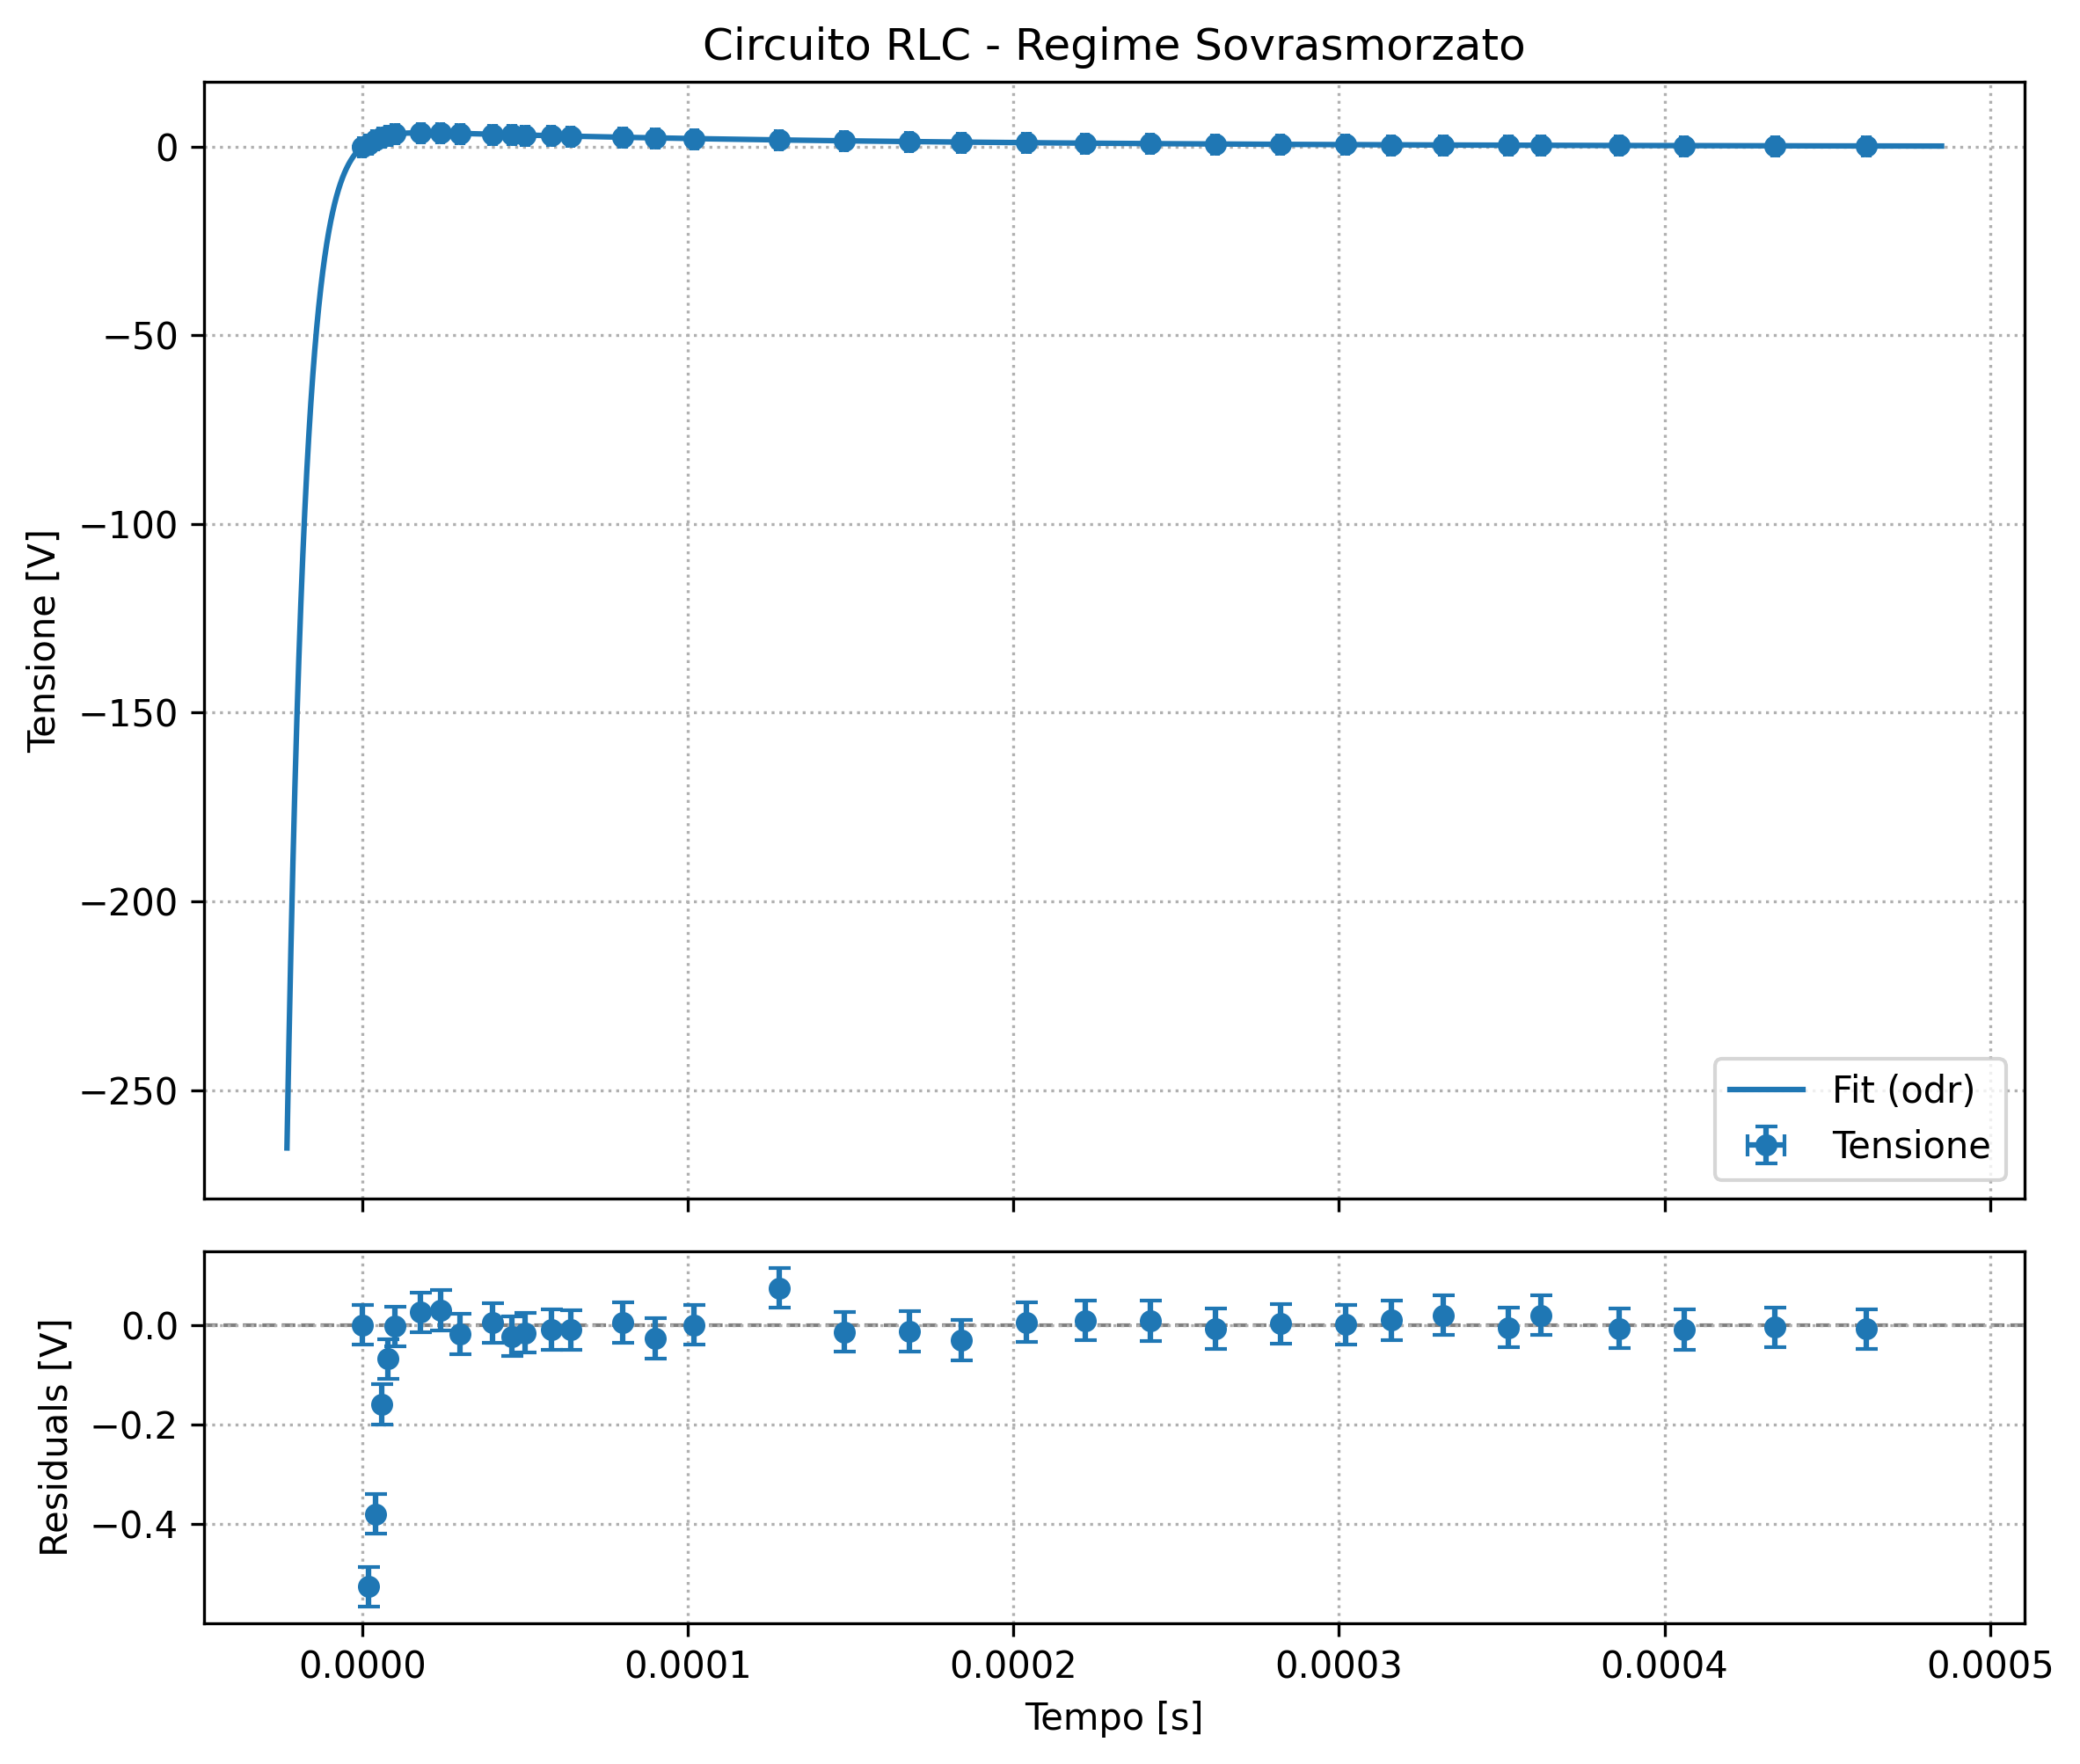
\includegraphics[width=0.9\linewidth]{grafici/sovrasmorzato.png}
    \captionof{figure}{Regime sovrasmorzato - Dati e Fit}
    \label{fig: rlc sovrasmorzato}
    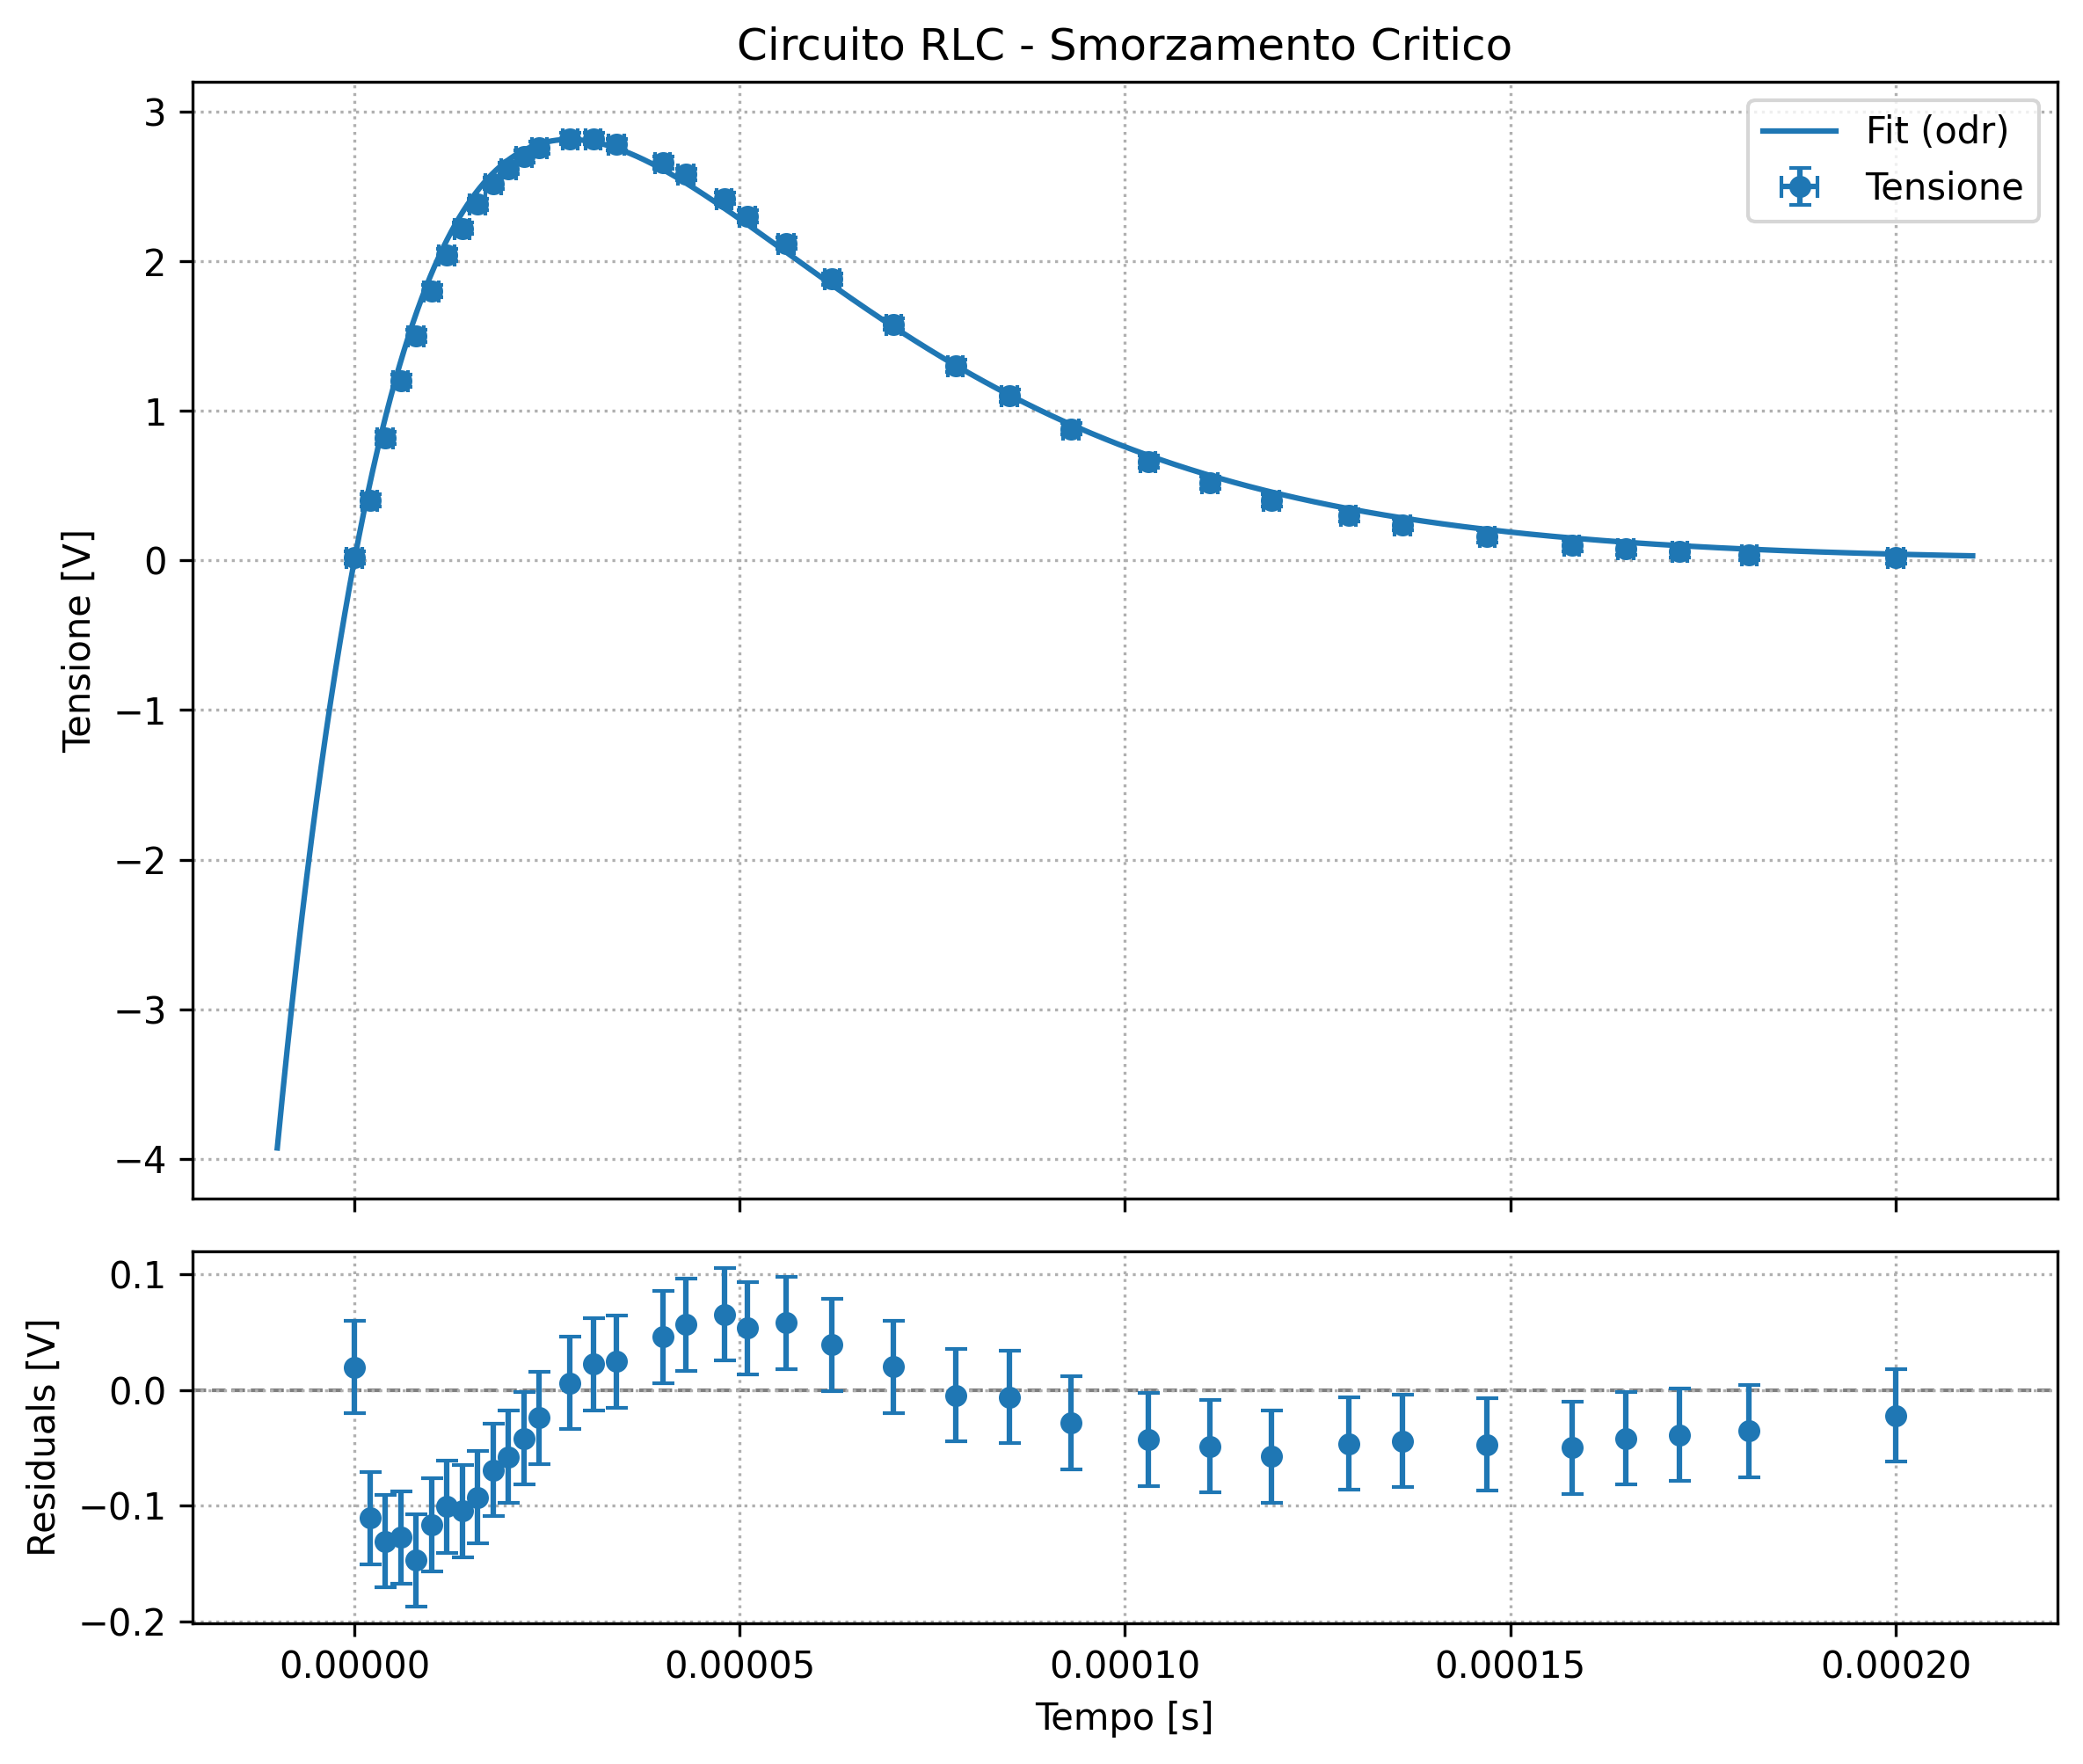
\includegraphics[width=0.9\linewidth]{grafici/critico.png}
    \captionof{figure}{Regime di smorzamento critico - Dati e Fit}
    \label{fig: rlc critico}
\end{center}

%tabelle parametri stimati RLC
\begin{table}[htbp]
\centering
\begin{tabular}{|l|cccccc|} % 'l' per Regime, 6 'c' per i parametri e risultati
\hline
Regime & $V_0$ & $\gamma$ & $\beta$ & $\chi^2$ & DoF & $\chi^2/\nu$ \\
\hline\hline
Sottosmorzato       & 94.6 ± 1.1 m     & 3.836 ± 0.055 k & 34.992 ± 0.047 k & 254  & 49 & 5.18  \\
Sovrasmorzato       & -4.345 ± 0.017   & 92.9 ± 2.6 k    & 85.9 ± 2.7 k     & 9.07 & 32 & 0.283 \\
Smorzamento Critico & 274.3 ± 2.6 k    & 35.86 ± 0.23 k  & -                & 29.2 & 35 & 0.834 \\ % Usato '-' per beta mancante
\hline
\end{tabular}
\caption{Parametri dei fit per i diversi regimi del circuito RLC.}
\label{tab:rlc_fit_results} % Label unico per la tabella unificata
\end{table}

Per valutare infine la bontà dei fit abbiamo utilizzato il test del chi quadro. I risultati ($\chi^2/\nu$) sono riportati nella Tabella \ref{tab:rlc_fit_results}.

\subsection{Conclusione}
Il test del chi quadro mostra accordo tra le misure realizzate e il fit stimato in caso di regime di sovrasmorzamento ($\chi^2/\nu = 0.283$) e smorzamento critico ($\chi^2/\nu = 0.834$). Per quanto riguarda invece il funzionamento del circuito RLC in regime sottosmorzato, i dati sperimentali non risultano in accordo con quanto ricavato dall'interpolazione, dato il valore elevato $\chi^2/\nu = 5.18$. Attribuiamo tale discrepanza alla difficoltà nel campionamento delle oscillazioni smorzate, specialmente in corrispondenza dei massimi e dei minimi. Il fatto che non riuscissimo a individuare esattamente la posizione dei punti stazionari si è in realtà verificato studiando tutti e 3 i regimi, ma ha influito soltanto sulla bontà del fit del regime sottosmorzato, in quanto la curva interpolata conteneva un numero significativo di massimi e minimi.


\section{Rettificatore di tensione}
\subsection{Obiettivo}
L'obiettivo dell'esperienza è creare un rettificatore di tensione ed osservare l'andamento della tensione nel tempo mediante l'oscilloscopio.

\subsection{Metodo}
Abbiamo realizzato un rettificatore a ponte di Graetz. Il circuito è composto da 4 diodi e un condensatore disposti come in figura. A differenza degli altri esperimenti in questo caso abbiamo sollecitato il circuito mediante un segnale sinusoidale.

\begin{figure}[htbp]
    \centering
    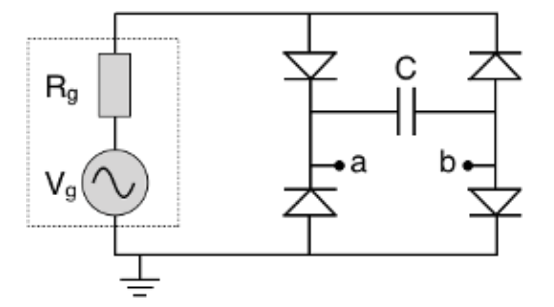
\includegraphics[width=0.7\textwidth]{grafici/image.png}
    \caption{Schema circuito rettificatore}
    \label{fig:rettificatore}
\end{figure}

A differenza di quanto rappresentato in figura, per eseguire l'esperimento abbiamo posizionato la sonda $b$ ai capi del generatore, in modo da osservare l'andamento della tensione generata e compararla a quella misurata all'interno rettificatore. 
\subsection{Osservazioni sperimentali}
Valutando l'andamento della tensione come illustrato precedentemente abbiamo osservato tale fenomeno:

\begin{figure}[htbp]
    \centering
    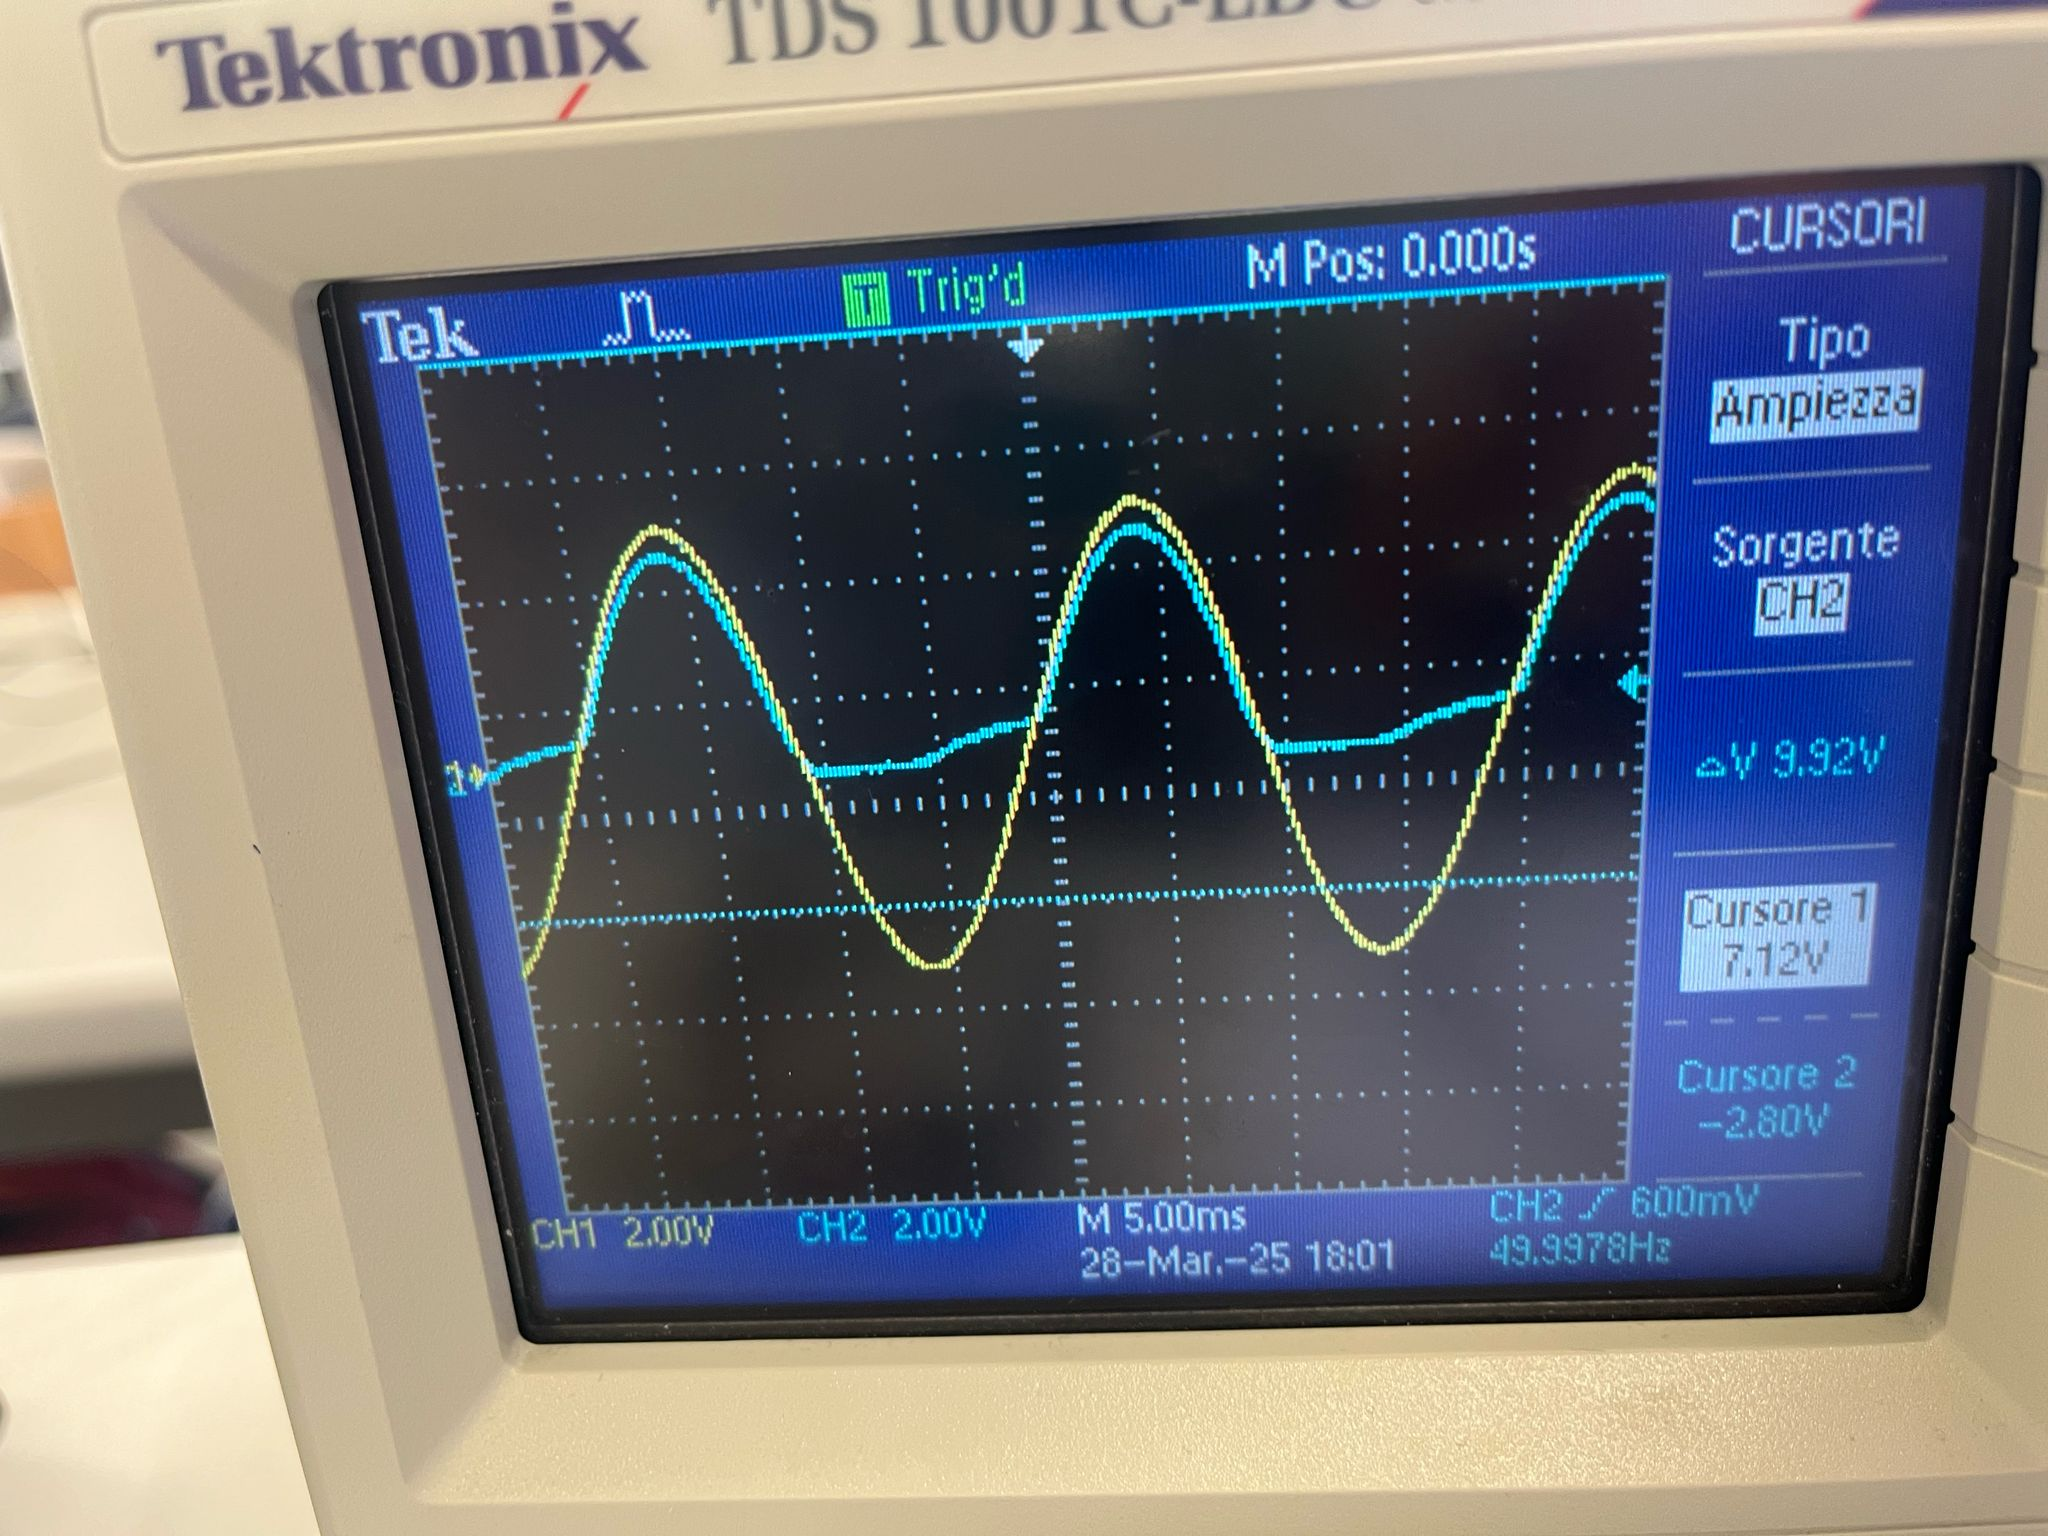
\includegraphics[width=0.7\textwidth]{grafici/rett_osc.jpg}
    \caption{Osservazione oscilloscopio}
    \label{fig:oscilloscopio}
\end{figure}

L'immagine rappresenta l'andamento della funzione tensione nel tempo, come restituito dall'oscilloscopio. La curva gialla rappresenta quanto misurato dalla sonda $b$, posizionata ai capi del generatore, mentre la curva blu rappresenta quanto misurato dalla sonda $a$, posizionata come nello schema in figura \ref{fig:rettificatore}. L'andamento osservato corrisponde all'andamento atteso: i diodi bloccano la parte negativa dell'onda e permettono il passaggio solamente di quella positiva. Se avessimo posizionato la sonda $b$ come in figura avremmo osservato un andamento simmetricamente opposto: la parte positiva sarebbe stata bloccata e la parte negativa sarebbe passata.



% Assumiamo ci sia del contenuto prima delle appendici
\newpage

\begin{appendices}
\renewcommand{\thetable}{\thesection.\arabic{table}} % Numera tabelle A.1, A.2, ...
\renewcommand{\thefigure}{\thesection.\arabic{figure}} % Numera figure A.1, A.2, ...

% ======================================================
\section{Dati Circuito RC} \label{app:dati_rc}
% ======================================================
\setcounter{table}{0} % Resetta contatore tabelle per questa sezione

% --- Tabelle RC affiancate ---
\begin{table}[htbp]
    \centering
    \begin{minipage}{0.48\textwidth}
        \centering\small % Riduci leggermente la dimensione del font se necessario
        \begin{tabular}{|c|c|}
        \hline
        Tempo & Tensione \\\hline\hline
        \num{-800 \pm 1} \si{\micro\second} & \num{292 \pm 4} \si{\milli\volt} \\
        \num{-740 \pm 1} \si{\micro\second} & \num{264 \pm 4} \si{\milli\volt} \\
        \num{-680 \pm 1} \si{\micro\second} & \num{228 \pm 4} \si{\milli\volt} \\
        \num{-620 \pm 1} \si{\micro\second} & \num{196 \pm 4} \si{\milli\volt} \\
        \num{-560 \pm 1} \si{\micro\second} & \num{164 \pm 4} \si{\milli\volt} \\
        \num{-500 \pm 1} \si{\micro\second} & \num{136 \pm 4} \si{\milli\volt} \\
        \num{-420 \pm 1} \si{\micro\second} & \num{104 \pm 4} \si{\milli\volt} \\
        \num{-340 \pm 1} \si{\micro\second} & \num{68 \pm 4} \si{\milli\volt} \\
        \num{-240 \pm 1} \si{\micro\second} & \num{32 \pm 4} \si{\milli\volt} \\
        \num{-160 \pm 1} \si{\micro\second} & \num{4 \pm 4} \si{\milli\volt} \\
        \num{-80 \pm 1} \si{\micro\second} & \num{-20 \pm 4} \si{\milli\volt} \\
        \num{20 \pm 1} \si{\micro\second} & \num{-48 \pm 4} \si{\milli\volt} \\
        \num{100 \pm 1} \si{\micro\second} & \num{-68 \pm 4} \si{\milli\volt} \\
        \num{200 \pm 1} \si{\micro\second} & \num{-92 \pm 4} \si{\milli\volt} \\
        \num{320 \pm 1} \si{\micro\second} & \num{-116 \pm 4} \si{\milli\volt} \\
        \num{440 \pm 1} \si{\micro\second} & \num{-136 \pm 4} \si{\milli\volt} \\
        \num{560 \pm 1} \si{\micro\second} & \num{-156 \pm 4} \si{\milli\volt} \\
        \num{700 \pm 1} \si{\micro\second} & \num{-176 \pm 4} \si{\milli\volt} \\
        \num{860 \pm 1} \si{\micro\second} & \num{-196 \pm 4} \si{\milli\volt} \\
        \num{1.02 \pm 0.01} \si{\milli\second} & \num{-212 \pm 4} \si{\milli\volt} \\ % Nota cambio unità tempo
        \num{1.30 \pm 0.01} \si{\milli\second} & \num{-236 \pm 4} \si{\milli\volt} \\
        \num{1.54 \pm 0.01} \si{\milli\second} & \num{-252 \pm 4} \si{\milli\volt} \\
        \num{1.72 \pm 0.01} \si{\milli\second} & \num{-260 \pm 4} \si{\milli\volt} \\
        \num{2.00 \pm 0.01} \si{\milli\second} & \num{-268 \pm 4} \si{\milli\volt} \\
        \num{2.38 \pm 0.01} \si{\milli\second} & \num{-280 \pm 4} \si{\milli\volt} \\
        \num{2.82 \pm 0.01} \si{\milli\second} & \num{-288 \pm 4} \si{\milli\volt} \\
        \hline
        \end{tabular}
        \caption{Dati RC: Scarica condensatore ($V_C(t)$).}
        \label{tab:rc_data_scarica_c}
    \end{minipage}\hfill % Spazio flessibile tra le minipage
    \begin{minipage}{0.48\textwidth}
        \centering\small % Riduci leggermente la dimensione del font se necessario
        \begin{tabular}{|c|c|}
        \hline
        Tempo & Tensione \\\hline\hline
        \num{4.22 \pm 0.01} \si{\milli\second} & \num{-296 \pm 4} \si{\milli\volt} \\
        \num{4.26 \pm 0.01} \si{\milli\second} & \num{-272 \pm 4} \si{\milli\volt} \\
        \num{4.34 \pm 0.01} \si{\milli\second} & \num{-228 \pm 4} \si{\milli\volt} \\
        \num{4.38 \pm 0.01} \si{\milli\second} & \num{-208 \pm 4} \si{\milli\volt} \\
        \num{4.42 \pm 0.01} \si{\milli\second} & \num{-184 \pm 4} \si{\milli\volt} \\
        \num{4.50 \pm 0.01} \si{\milli\second} & \num{-148 \pm 4} \si{\milli\volt} \\
        \num{4.54 \pm 0.01} \si{\milli\second} & \num{-128 \pm 4} \si{\milli\volt} \\
        \num{4.58 \pm 0.01} \si{\milli\second} & \num{-108 \pm 4} \si{\milli\volt} \\
        \num{4.64 \pm 0.01} \si{\milli\second} & \num{-88 \pm 4} \si{\milli\volt} \\
        \num{4.76 \pm 0.01} \si{\milli\second} & \num{-40 \pm 4} \si{\milli\volt} \\
        \num{4.82 \pm 0.01} \si{\milli\second} & \num{-20 \pm 4} \si{\milli\volt} \\
        \num{4.92 \pm 0.01} \si{\milli\second} & \num{12 \pm 4} \si{\milli\volt} \\
        \num{5.02 \pm 0.01} \si{\milli\second} & \num{40 \pm 4} \si{\milli\volt} \\
        \num{5.12 \pm 0.01} \si{\milli\second} & \num{64 \pm 4} \si{\milli\volt} \\
        \num{5.20 \pm 0.01} \si{\milli\second} & \num{80 \pm 4} \si{\milli\volt} \\
        \num{5.30 \pm 0.01} \si{\milli\second} & \num{104 \pm 4} \si{\milli\volt} \\
        \num{5.46 \pm 0.01} \si{\milli\second} & \num{132 \pm 4} \si{\milli\volt} \\
        \num{5.54 \pm 0.01} \si{\milli\second} & \num{144 \pm 4} \si{\milli\volt} \\
        \num{5.66 \pm 0.01} \si{\milli\second} & \num{164 \pm 4} \si{\milli\volt} \\
        \num{5.78 \pm 0.01} \si{\milli\second} & \num{180 \pm 4} \si{\milli\volt} \\
        \num{5.94 \pm 0.01} \si{\milli\second} & \num{196 \pm 4} \si{\milli\volt} \\
        \num{6.06 \pm 0.01} \si{\milli\second} & \num{208 \pm 4} \si{\milli\volt} \\
        \num{6.32 \pm 0.01} \si{\milli\second} & \num{228 \pm 4} \si{\milli\volt} \\
        \num{6.54 \pm 0.01} \si{\milli\second} & \num{240 \pm 4} \si{\milli\volt} \\
        \num{6.80 \pm 0.01} \si{\milli\second} & \num{252 \pm 4} \si{\milli\volt} \\
        \num{7.02 \pm 0.01} \si{\milli\second} & \num{260 \pm 4} \si{\milli\volt} \\
        \num{7.38 \pm 0.01} \si{\milli\second} & \num{272 \pm 4} \si{\milli\volt} \\
        \num{7.82 \pm 0.01} \si{\milli\second} & \num{280 \pm 4} \si{\milli\volt} \\
        \num{8.28 \pm 0.01} \si{\milli\second} & \num{284 \pm 4} \si{\milli\volt} \\
        \num{8.78 \pm 0.01} \si{\milli\second} & \num{288 \pm 4} \si{\milli\volt} \\
        \hline
        \end{tabular}
        \caption{Dati RC: Carica condensatore ($V_C(t)$).}
        \label{tab:rc_data_carica_c}
    \end{minipage}
\end{table}

\begin{table}[htbp]
    \centering
    \begin{minipage}{0.48\textwidth}
        \centering\small % Riduci leggermente la dimensione del font se necessario
        \begin{tabular}{|c|c|}
        \hline
        Tempo & Tensione \\\hline\hline
        \num{20 \pm 1} \si{\micro\second} & \num{576 \pm 4} \si{\milli\volt} \\
        \num{80 \pm 1} \si{\micro\second} & \num{540 \pm 4} \si{\milli\volt} \\
        \num{180 \pm 1} \si{\micro\second} & \num{492 \pm 4} \si{\milli\volt} \\
        \num{260 \pm 1} \si{\micro\second} & \num{452 \pm 4} \si{\milli\volt} \\
        \num{340 \pm 1} \si{\micro\second} & \num{412 \pm 4} \si{\milli\volt} \\
        \num{420 \pm 1} \si{\micro\second} & \num{380 \pm 4} \si{\milli\volt} \\
        \num{520 \pm 1} \si{\micro\second} & \num{344 \pm 4} \si{\milli\volt} \\
        \num{600 \pm 1} \si{\micro\second} & \num{316 \pm 4} \si{\milli\volt} \\
        \num{700 \pm 1} \si{\micro\second} & \num{288 \pm 4} \si{\milli\volt} \\
        \num{820 \pm 1} \si{\micro\second} & \num{248 \pm 4} \si{\milli\volt} \\
        \num{920 \pm 1} \si{\micro\second} & \num{224 \pm 4} \si{\milli\volt} \\
        \num{1.02 \pm 0.01} \si{\milli\second} & \num{204 \pm 4} \si{\milli\volt} \\ % Nota cambio unità tempo
        \num{1.12 \pm 0.01} \si{\milli\second} & \num{184 \pm 4} \si{\milli\volt} \\
        \num{1.24 \pm 0.01} \si{\milli\second} & \num{160 \pm 4} \si{\milli\volt} \\
        \num{1.46 \pm 0.01} \si{\milli\second} & \num{124 \pm 4} \si{\milli\volt} \\
        \num{1.68 \pm 0.01} \si{\milli\second} & \num{100 \pm 4} \si{\milli\volt} \\
        \num{1.80 \pm 0.01} \si{\milli\second} & \num{84 \pm 4} \si{\milli\volt} \\
        \num{1.96 \pm 0.01} \si{\milli\second} & \num{72 \pm 4} \si{\milli\volt} \\
        \num{2.08 \pm 0.01} \si{\milli\second} & \num{68 \pm 4} \si{\milli\volt} \\
        \num{2.20 \pm 0.01} \si{\milli\second} & \num{60 \pm 4} \si{\milli\volt} \\
        \num{2.32 \pm 0.01} \si{\milli\second} & \num{52 \pm 4} \si{\milli\volt} \\
        \num{2.44 \pm 0.01} \si{\milli\second} & \num{48 \pm 4} \si{\milli\volt} \\
        \num{2.60 \pm 0.01} \si{\milli\second} & \num{36 \pm 4} \si{\milli\volt} \\
        \num{2.80 \pm 0.01} \si{\milli\second} & \num{28 \pm 4} \si{\milli\volt} \\
        \num{2.96 \pm 0.01} \si{\milli\second} & \num{24 \pm 4} \si{\milli\volt} \\
        \num{3.16 \pm 0.01} \si{\milli\second} & \num{16 \pm 4} \si{\milli\volt} \\
        \num{3.40 \pm 0.01} \si{\milli\second} & \num{12 \pm 4} \si{\milli\volt} \\
        \num{3.60 \pm 0.01} \si{\milli\second} & \num{10 \pm 4} \si{\milli\volt} \\
        \hline
        \end{tabular}
        \caption{Dati RC: Carica resistenza ($V_R(t)$).}
        \label{tab:rc_data_carica_r}
    \end{minipage}\hfill % Spazio flessibile
    \begin{minipage}{0.48\textwidth}
        \centering\small % Riduci leggermente la dimensione del font se necessario
        \begin{tabular}{|c|c|}
        \hline
        Tempo & Tensione \\\hline\hline
        \num{5.00 \pm 0.01} \si{\milli\second} & \num{-588 \pm 4} \si{\milli\volt} \\
        \num{5.06 \pm 0.01} \si{\milli\second} & \num{-552 \pm 4} \si{\milli\volt} \\
        \num{5.12 \pm 0.01} \si{\milli\second} & \num{-520 \pm 4} \si{\milli\volt} \\
        \num{5.20 \pm 0.01} \si{\milli\second} & \num{-480 \pm 4} \si{\milli\volt} \\
        \num{5.24 \pm 0.01} \si{\milli\second} & \num{-456 \pm 4} \si{\milli\volt} \\
        \num{5.30 \pm 0.01} \si{\milli\second} & \num{-428 \pm 4} \si{\milli\volt} \\
        \num{5.36 \pm 0.01} \si{\milli\second} & \num{-400 \pm 4} \si{\milli\volt} \\
        \num{5.40 \pm 0.01} \si{\milli\second} & \num{-388 \pm 4} \si{\milli\volt} \\
        \num{5.48 \pm 0.01} \si{\milli\second} & \num{-356 \pm 4} \si{\milli\volt} \\
        \num{5.50 \pm 0.01} \si{\milli\second} & \num{-348 \pm 4} \si{\milli\volt} \\
        \num{5.54 \pm 0.01} \si{\milli\second} & \num{-332 \pm 4} \si{\milli\volt} \\
        \num{5.60 \pm 0.01} \si{\milli\second} & \num{-312 \pm 4} \si{\milli\volt} \\
        \num{5.64 \pm 0.01} \si{\milli\second} & \num{-300 \pm 4} \si{\milli\volt} \\
        \num{5.72 \pm 0.01} \si{\milli\second} & \num{-276 \pm 4} \si{\milli\volt} \\
        \num{5.78 \pm 0.01} \si{\milli\second} & \num{-260 \pm 4} \si{\milli\volt} \\
        \num{5.86 \pm 0.01} \si{\milli\second} & \num{-240 \pm 4} \si{\milli\volt} \\
        \num{5.90 \pm 0.01} \si{\milli\second} & \num{-224 \pm 4} \si{\milli\volt} \\
        \num{5.94 \pm 0.01} \si{\milli\second} & \num{-220 \pm 4} \si{\milli\volt} \\
        \num{6.00 \pm 0.01} \si{\milli\second} & \num{-204 \pm 4} \si{\milli\volt} \\
        \num{6.10 \pm 0.01} \si{\milli\second} & \num{-184 \pm 4} \si{\milli\volt} \\
        \num{6.16 \pm 0.01} \si{\milli\second} & \num{-176 \pm 4} \si{\milli\volt} \\
        \num{6.22 \pm 0.01} \si{\milli\second} & \num{-164 \pm 4} \si{\milli\volt} \\
        \num{6.40 \pm 0.01} \si{\milli\second} & \num{-132 \pm 4} \si{\milli\volt} \\
        \num{6.52 \pm 0.01} \si{\milli\second} & \num{-116 \pm 4} \si{\milli\volt} \\
        \num{6.72 \pm 0.01} \si{\milli\second} & \num{-96 \pm 4} \si{\milli\volt} \\
        \num{6.80 \pm 0.01} \si{\milli\second} & \num{-88 \pm 4} \si{\milli\volt} \\
        \num{6.92 \pm 0.01} \si{\milli\second} & \num{-76 \pm 4} \si{\milli\volt} \\
        \num{7.08 \pm 0.01} \si{\milli\second} & \num{-64 \pm 4} \si{\milli\volt} \\
        \num{7.22 \pm 0.01} \si{\milli\second} & \num{-56 \pm 4} \si{\milli\volt} \\
        \num{7.38 \pm 0.01} \si{\milli\second} & \num{-48 \pm 4} \si{\milli\volt} \\
        \num{7.52 \pm 0.01} \si{\milli\second} & \num{-40 \pm 4} \si{\milli\volt} \\
        \num{7.62 \pm 0.01} \si{\milli\second} & \num{-36 \pm 4} \si{\milli\volt} \\
        \num{7.78 \pm 0.01} \si{\milli\second} & \num{-32 \pm 4} \si{\milli\volt} \\
        \num{7.98 \pm 0.01} \si{\milli\second} & \num{-24 \pm 4} \si{\milli\volt} \\
        \num{8.28 \pm 0.01} \si{\milli\second} & \num{-20 \pm 4} \si{\milli\volt} \\
        \num{8.42 \pm 0.01} \si{\milli\second} & \num{-16 \pm 4} \si{\milli\volt} \\
        \num{8.66 \pm 0.01} \si{\milli\second} & \num{-12 \pm 4} \si{\milli\volt} \\
        \num{8.82 \pm 0.01} \si{\milli\second} & \num{-8 \pm 4} \si{\milli\volt} \\
        \hline
        \end{tabular}
        \caption{Dati RC: Scarica resistenza ($V_R(t)$).}
        \label{tab:rc_data_scarica_r}
    \end{minipage}
\end{table}

\newpage % Probabilmente vuoi una nuova pagina prima della sezione RL

% ======================================================
\section{Dati Circuito RL} \label{app:dati_rl}
% ======================================================
\setcounter{table}{0} % Resetta contatore tabelle per questa sezione

% --- Tabelle RL affiancate (formato simile all'originale ma con unità per cella) ---
\begin{table}[htbp]
    \centering
    \begin{minipage}{0.48\textwidth} % Leggermente più largo per contenuto
        \centering\small
        \begin{tabular}{|c|c|}
        \hline
        \( t \) & \( V_L(t) \) \\ % Header senza unità
        \hline\hline
        \num{0   \pm 10} \si{\micro\second} & \num{-248 \pm 2} \si{\milli\volt} \\
        \num{8   \pm 10} \si{\micro\second} & \num{-224 \pm 2} \si{\milli\volt} \\
        \num{16  \pm 10} \si{\micro\second} & \num{-196 \pm 2} \si{\milli\volt} \\
        \num{24  \pm 10} \si{\micro\second} & \num{-172 \pm 2} \si{\milli\volt} \\
        \num{32  \pm 10} \si{\micro\second} & \num{-148 \pm 2} \si{\milli\volt} \\
        \num{40  \pm 10} \si{\micro\second} & \num{-128 \pm 2} \si{\milli\volt} \\
        \num{48  \pm 10} \si{\micro\second} & \num{-108 \pm 2} \si{\milli\volt} \\
        \num{56  \pm 10} \si{\micro\second} & \num{-88  \pm 2} \si{\milli\volt} \\
        \num{64  \pm 10} \si{\micro\second} & \num{-68  \pm 2} \si{\milli\volt} \\
        \num{72  \pm 10} \si{\micro\second} & \num{-52  \pm 2} \si{\milli\volt} \\
        \num{92  \pm 10} \si{\micro\second} & \num{-12  \pm 2} \si{\milli\volt} \\
        \num{100 \pm 10} \si{\micro\second} & \num{0    \pm 2} \si{\milli\volt} \\
        \num{108 \pm 10} \si{\micro\second} & \num{16   \pm 2} \si{\milli\volt} \\
        \num{116 \pm 10} \si{\micro\second} & \num{28   \pm 2} \si{\milli\volt} \\
        \num{132 \pm 10} \si{\micro\second} & \num{52   \pm 2} \si{\milli\volt} \\
        \num{148 \pm 10} \si{\micro\second} & \num{72   \pm 2} \si{\milli\volt} \\
        \num{160 \pm 10} \si{\micro\second} & \num{88   \pm 2} \si{\milli\volt} \\
        \num{180 \pm 10} \si{\micro\second} & \num{108  \pm 2} \si{\milli\volt} \\
        \num{192 \pm 10} \si{\micro\second} & \num{120  \pm 2} \si{\milli\volt} \\
        \num{208 \pm 10} \si{\micro\second} & \num{132  \pm 2} \si{\milli\volt} \\
        \num{224 \pm 10} \si{\micro\second} & \num{144  \pm 2} \si{\milli\volt} \\
        \num{236 \pm 10} \si{\micro\second} & \num{152  \pm 2} \si{\milli\volt} \\
        \num{252 \pm 10} \si{\micro\second} & \num{164  \pm 2} \si{\milli\volt} \\
        \num{264 \pm 10} \si{\micro\second} & \num{168  \pm 2} \si{\milli\volt} \\
        \num{280 \pm 10} \si{\micro\second} & \num{176  \pm 2} \si{\milli\volt} \\
        \num{304 \pm 10} \si{\micro\second} & \num{188  \pm 2} \si{\milli\volt} \\
        \num{324 \pm 10} \si{\micro\second} & \num{196  \pm 2} \si{\milli\volt} \\
        \num{364 \pm 10} \si{\micro\second} & \num{208  \pm 2} \si{\milli\volt} \\
        \num{412 \pm 10} \si{\micro\second} & \num{220  \pm 2} \si{\milli\volt} \\
        \num{448 \pm 10} \si{\micro\second} & \num{224  \pm 2} \si{\milli\volt} \\
        \num{488 \pm 10} \si{\micro\second} & \num{228  \pm 2} \si{\milli\volt} \\
        \num{516 \pm 10} \si{\micro\second} & \num{232  \pm 2} \si{\milli\volt} \\
        \num{556 \pm 10} \si{\micro\second} & \num{236  \pm 2} \si{\milli\volt} \\
        \num{604 \pm 10} \si{\micro\second} & \num{240  \pm 2} \si{\milli\volt} \\
        \hline
        \end{tabular}
        \caption{Dati RL: Tempo e Tensione dell'Induttore (scarica).}
        \label{tab:rl_data_scarica_l}
    \end{minipage}\hfill
    \begin{minipage}{0.48\textwidth} % Leggermente più largo per contenuto
        \centering\small
        \begin{tabular}{|c|c|}
        \hline
         \( t \) & \( V_L(t) \) \\ % Header senza unità
        \hline\hline
        \num{3.05  \pm 0.01} \si{\milli\second} & \num{248 \pm 2} \si{\milli\volt} \\
        \num{3.07  \pm 0.01} \si{\milli\second} & \num{212 \pm 2} \si{\milli\volt} \\
        \num{3.09  \pm 0.01} \si{\milli\second} & \num{152 \pm 2} \si{\milli\volt} \\
        \num{3.11  \pm 0.01} \si{\milli\second} & \num{96  \pm 2} \si{\milli\volt} \\
        \num{3.13  \pm 0.01} \si{\milli\second} & \num{48  \pm 2} \si{\milli\volt} \\
        \num{3.16  \pm 0.01} \si{\milli\second} & \num{-8  \pm 2} \si{\milli\volt} \\
        \num{3.18  \pm 0.01} \si{\milli\second} & \num{-40 \pm 2} \si{\milli\volt} \\
        \num{3.21  \pm 0.01} \si{\milli\second} & \num{-80 \pm 2} \si{\milli\volt} \\
        \num{3.22  \pm 0.01} \si{\milli\second} & \num{-92 \pm 2} \si{\milli\volt} \\
        \num{3.24  \pm 0.01} \si{\milli\second} & \num{-112 \pm 2} \si{\milli\volt} \\
        \num{3.29  \pm 0.01} \si{\milli\second} & \num{-152 \pm 2} \si{\milli\volt} \\
        \num{3.32  \pm 0.01} \si{\milli\second} & \num{-172 \pm 2} \si{\milli\volt} \\
        \num{3.36  \pm 0.01} \si{\milli\second} & \num{-192 \pm 2} \si{\milli\volt} \\
        \num{3.40  \pm 0.01} \si{\milli\second} & \num{-208 \pm 2} \si{\milli\volt} \\
        \num{3.44  \pm 0.01} \si{\milli\second} & \num{-216 \pm 2} \si{\milli\volt} \\
        \num{3.49  \pm 0.01} \si{\milli\second} & \num{-228 \pm 2} \si{\milli\volt} \\
        \num{3.54  \pm 0.01} \si{\milli\second} & \num{-232 \pm 2} \si{\milli\volt} \\
        \num{3.59  \pm 0.01} \si{\milli\second} & \num{-240 \pm 2} \si{\milli\volt} \\
        \num{3.62  \pm 0.01} \si{\milli\second} & \num{-240 \pm 2} \si{\milli\volt} \\
        \num{3.77  \pm 0.01} \si{\milli\second} & \num{-248 \pm 2} \si{\milli\volt} \\
        \hline
        % Aggiungi righe vuote se necessario per allineare verticalmente
        \multicolumn{2}{c}{\rule{0pt}{25.5ex}} % Spazio vuoto per allineare con tabella sinistra più lunga
        % Ripeti \rule{0pt}{...} per altre righe se necessario
        \end{tabular}
       \caption{Dati RL: Tempo e Tensione dell'Induttore (carica).}
       \label{tab:rl_data_carica_l}
    \end{minipage}
\end{table}

\begin{table}[htbp]
    \centering
    \begin{minipage}{0.48\textwidth} % Leggermente più largo
        \centering\small
        \begin{tabular}{|c|c|}
        \hline
         \( t \) & \( V_R(t) \) \\ % Header senza unità
        \hline\hline
        \num{0    \pm 10} \si{\micro\second} & \num{552  \pm 2} \si{\milli\volt} \\
        \num{40   \pm 10} \si{\micro\second} & \num{424  \pm 2} \si{\milli\volt} \\
        \num{60   \pm 10} \si{\micro\second} & \num{368  \pm 2} \si{\milli\volt} \\
        \num{80   \pm 10} \si{\micro\second} & \num{324  \pm 2} \si{\milli\volt} \\
        \num{100  \pm 10} \si{\micro\second} & \num{284  \pm 2} \si{\milli\volt} \\
        \num{140  \pm 10} \si{\micro\second} & \num{220  \pm 2} \si{\milli\volt} \\
        \num{180  \pm 10} \si{\micro\second} & \num{172  \pm 2} \si{\milli\volt} \\
        \num{200  \pm 10} \si{\micro\second} & \num{152  \pm 2} \si{\milli\volt} \\
        \num{240  \pm 10} \si{\micro\second} & \num{120  \pm 2} \si{\milli\volt} \\
        \num{280  \pm 10} \si{\micro\second} & \num{100  \pm 2} \si{\milli\volt} \\
        \num{320  \pm 10} \si{\micro\second} & \num{80   \pm 2} \si{\milli\volt} \\
        \num{360  \pm 10} \si{\micro\second} & \num{68   \pm 2} \si{\milli\volt} \\
        \num{400  \pm 10} \si{\micro\second} & \num{56   \pm 2} \si{\milli\volt} \\
        \num{440  \pm 10} \si{\micro\second} & \num{48   \pm 2} \si{\milli\volt} \\
        \num{480  \pm 10} \si{\micro\second} & \num{44   \pm 2} \si{\milli\volt} \\
        \num{500  \pm 10} \si{\micro\second} & \num{40   \pm 2} \si{\milli\volt} \\
        \num{540  \pm 10} \si{\micro\second} & \num{36   \pm 2} \si{\milli\volt} \\
        \num{580  \pm 10} \si{\micro\second} & \num{36   \pm 2} \si{\milli\volt} \\
        \num{600  \pm 10} \si{\micro\second} & \num{32   \pm 2} \si{\milli\volt} \\
        \num{700  \pm 10} \si{\micro\second} & \num{28   \pm 2} \si{\milli\volt} \\
        \hline
         % Aggiungi righe vuote se necessario per allineare verticalmente
        \multicolumn{2}{c}{\rule{0pt}{10ex}} % Spazio vuoto
        \end{tabular}
        \caption{Dati RL: Tempo e Tensione della Resistenza (scarica).}
        \label{tab:rl_data_scarica_r}
    \end{minipage}\hfill
    \begin{minipage}{0.48\textwidth} % Leggermente più largo
        \centering\small
        \begin{tabular}{|c|c|}
        \hline
         \( t \) & \( V_R(t) \) \\ % Header senza unità
        \hline\hline
        \num{3.06  \pm 0.02} \si{\milli\second} & \num{-572 \pm 2} \si{\milli\volt} \\
        \num{3.08  \pm 0.02} \si{\milli\second} & \num{-500 \pm 2} \si{\milli\volt} \\
        \num{3.10  \pm 0.02} \si{\milli\second} & \num{-436 \pm 2} \si{\milli\volt} \\
        \num{3.12  \pm 0.02} \si{\milli\second} & \num{-380 \pm 2} \si{\milli\volt} \\
        \num{3.14  \pm 0.02} \si{\milli\second} & \num{-336 \pm 2} \si{\milli\volt} \\
        \num{3.16  \pm 0.02} \si{\milli\second} & \num{-296 \pm 2} \si{\milli\volt} \\
        \num{3.18  \pm 0.02} \si{\milli\second} & \num{-260 \pm 2} \si{\milli\volt} \\
        \num{3.20  \pm 0.02} \si{\milli\second} & \num{-228 \pm 2} \si{\milli\volt} \\
        \num{3.22  \pm 0.02} \si{\milli\second} & \num{-200 \pm 2} \si{\milli\volt} \\
        \num{3.24  \pm 0.02} \si{\milli\second} & \num{-176 \pm 2} \si{\milli\volt} \\
        \num{3.26  \pm 0.02} \si{\milli\second} & \num{-160 \pm 2} \si{\milli\volt} \\
        \num{3.30  \pm 0.02} \si{\milli\second} & \num{-124 \pm 2} \si{\milli\volt} \\
        \num{3.33  \pm 0.02} \si{\milli\second} & \num{-108 \pm 2} \si{\milli\volt} \\
        \num{3.36  \pm 0.02} \si{\milli\second} & \num{-92  \pm 2} \si{\milli\volt} \\
        \num{3.39  \pm 0.02} \si{\milli\second} & \num{-80  \pm 2} \si{\milli\volt} \\
        \num{3.44  \pm 0.02} \si{\milli\second} & \num{-64  \pm 2} \si{\milli\volt} \\
        \num{3.47  \pm 0.02} \si{\milli\second} & \num{-56  \pm 2} \si{\milli\volt} \\
        \num{3.50  \pm 0.02} \si{\milli\second} & \num{-52  \pm 2} \si{\milli\volt} \\
        \num{3.54  \pm 0.02} \si{\milli\second} & \num{-44  \pm 2} \si{\milli\volt} \\
        \num{3.59  \pm 0.02} \si{\milli\second} & \num{-40  \pm 2} \si{\milli\volt} \\
        \num{3.64  \pm 0.02} \si{\milli\second} & \num{-36  \pm 2} \si{\milli\volt} \\
        \num{3.66  \pm 0.02} \si{\milli\second} & \num{-36  \pm 2} \si{\milli\volt} \\
        \num{3.67  \pm 0.02} \si{\milli\second} & \num{-32  \pm 2} \si{\milli\volt} \\
        \num{3.80  \pm 0.02} \si{\milli\second} & \num{-28  \pm 2} \si{\milli\volt} \\
        \hline
        \end{tabular}
       \caption{Dati RL: Tempo e Tensione della Resistenza (carica).}
       \label{tab:rl_data_carica_r}
    \end{minipage}
\end{table}

\newpage % Probabilmente vuoi una nuova pagina prima della sezione RLC

% ======================================================
\section{Dati Circuito RLC} \label{app:dati_rlc}
% ======================================================
\setcounter{table}{0} % Resetta contatore tabelle per questa sezione

% --- Tabelle RLC affiancate (prime due) ---
\begin{table}[htbp]
    \centering
    \begin{minipage}{0.48\textwidth}
        \centering\small
        \begin{tabular}{|c|c|}
        \hline
        Tempo & Tensione \\\hline\hline % Tolte unità da header
        \num{0 \pm 1} \si{\micro\second} & \num{1.2 \pm 0.4} \si{\milli\volt} \\
        \num{16 \pm 1} \si{\micro\second} & \num{45.4 \pm 0.4} \si{\milli\volt} \\
        \num{24 \pm 1} \si{\micro\second} & \num{63.2 \pm 0.4} \si{\milli\volt} \\
        \num{44 \pm 1} \si{\micro\second} & \num{80.8 \pm 0.4} \si{\milli\volt} \\
        \num{60 \pm 1} \si{\micro\second} & \num{67.6 \pm 0.4} \si{\milli\volt} \\
        \num{72 \pm 1} \si{\micro\second} & \num{45.6 \pm 0.4} \si{\milli\volt} \\
        \num{88 \pm 1} \si{\micro\second} & \num{8.8 \pm 0.4} \si{\milli\volt} \\
        \num{96 \pm 1} \si{\micro\second} & \num{-8.8 \pm 0.4} \si{\milli\volt} \\
        \num{120 \pm 1} \si{\micro\second} & \num{-48.0 \pm 0.4} \si{\milli\volt} \\
        \num{136 \pm 1} \si{\micro\second} & \num{-52.8 \pm 0.4} \si{\milli\volt} \\
        \num{148 \pm 1} \si{\micro\second} & \num{-46.4 \pm 0.4} \si{\milli\volt} \\
        \num{160 \pm 1} \si{\micro\second} & \num{-32.0 \pm 0.4} \si{\milli\volt} \\
        \num{172 \pm 1} \si{\micro\second} & \num{-12.4 \pm 0.4} \si{\milli\volt} \\
        \num{184 \pm 1} \si{\micro\second} & \num{7.6 \pm 0.4} \si{\milli\volt} \\
        \num{200 \pm 1} \si{\micro\second} & \num{28.8 \pm 0.4} \si{\milli\volt} \\
        \num{224 \pm 1} \si{\micro\second} & \num{41.0 \pm 0.4} \si{\milli\volt} \\ % Era 41.0
        \num{244 \pm 1} \si{\micro\second} & \num{30.4 \pm 0.4} \si{\milli\volt} \\
        \num{260 \pm 1} \si{\micro\second} & \num{12.8 \pm 0.4} \si{\milli\volt} \\
        \num{276 \pm 1} \si{\micro\second} & \num{-5.6 \pm 0.4} \si{\milli\volt} \\
        \num{288 \pm 1} \si{\micro\second} & \num{-17.6 \pm 0.4} \si{\milli\volt} \\
        \num{312 \pm 1} \si{\micro\second} & \num{-27.2 \pm 0.4} \si{\milli\volt} \\
        \num{332 \pm 1} \si{\micro\second} & \num{-20.4 \pm 0.4} \si{\milli\volt} \\
        \num{348 \pm 1} \si{\micro\second} & \num{-8.8 \pm 0.4} \si{\milli\volt} \\
        \num{364 \pm 1} \si{\micro\second} & \num{4.8 \pm 0.4} \si{\milli\volt} \\
        \num{380 \pm 1} \si{\micro\second} & \num{15.2 \pm 0.4} \si{\milli\volt} \\
        \num{404 \pm 1} \si{\micro\second} & \num{20.8 \pm 0.4} \si{\milli\volt} \\
        \num{420 \pm 1} \si{\micro\second} & \num{17.2 \pm 0.4} \si{\milli\volt} \\
        \num{436 \pm 1} \si{\micro\second} & \num{8.8 \pm 0.4} \si{\milli\volt} \\
        \num{444 \pm 1} \si{\micro\second} & \num{4.0 \pm 0.4} \si{\milli\volt} \\
        \num{456 \pm 1} \si{\micro\second} & \num{-3.2 \pm 0.4} \si{\milli\volt} \\
        \num{468 \pm 1} \si{\micro\second} & \num{-8.8 \pm 0.4} \si{\milli\volt} \\
        \num{488 \pm 1} \si{\micro\second} & \num{-13.6 \pm 0.4} \si{\milli\volt} \\
        \num{516 \pm 1} \si{\micro\second} & \num{-8.0 \pm 0.4} \si{\milli\volt} \\
        \num{528 \pm 1} \si{\micro\second} & \num{-3.2 \pm 0.4} \si{\milli\volt} \\
        \num{540 \pm 1} \si{\micro\second} & \num{2.0 \pm 0.4} \si{\milli\volt} \\
        \num{552 \pm 1} \si{\micro\second} & \num{6.4 \pm 0.4} \si{\milli\volt} \\
        \num{580 \pm 1} \si{\micro\second} & \num{11.6 \pm 0.4} \si{\milli\volt} \\
        \num{608 \pm 1} \si{\micro\second} & \num{7.2 \pm 0.4} \si{\milli\volt} \\
        \num{624 \pm 1} \si{\micro\second} & \num{2.0 \pm 0.4} \si{\milli\volt} \\
        \num{640 \pm 1} \si{\micro\second} & \num{-2.4 \pm 0.4} \si{\milli\volt} \\
        \num{672 \pm 1} \si{\micro\second} & \num{-6.4 \pm 0.4} \si{\milli\volt} \\
        \num{692 \pm 1} \si{\micro\second} & \num{-4.0 \pm 0.4} \si{\milli\volt} \\
        \num{704 \pm 1} \si{\micro\second} & \num{-1.2 \pm 0.4} \si{\milli\volt} \\
        \num{720 \pm 1} \si{\micro\second} & \num{2.0 \pm 0.4} \si{\milli\volt} \\
        \num{736 \pm 1} \si{\micro\second} & \num{4.4 \pm 0.4} \si{\milli\volt} \\
        \num{760 \pm 1} \si{\micro\second} & \num{6.4 \pm 0.4} \si{\milli\volt} \\
        \num{776 \pm 1} \si{\micro\second} & \num{5.6 \pm 0.4} \si{\milli\volt} \\
        \num{788 \pm 1} \si{\micro\second} & \num{4.0 \pm 0.4} \si{\milli\volt} \\
        \num{800 \pm 1} \si{\micro\second} & \num{2.0 \pm 0.4} \si{\milli\volt} \\
        \num{816 \pm 1} \si{\micro\second} & \num{-0.4 \pm 0.4} \si{\milli\volt} \\ % Corretto uV -> mV
        \num{832 \pm 1} \si{\micro\second} & \num{-2.0 \pm 0.4} \si{\milli\volt} \\
        \num{852 \pm 1} \si{\micro\second} & \num{-2.8 \pm 0.4} \si{\milli\volt} \\
        \hline
        \end{tabular}
        \caption{Dati RLC: Regime sottosmorzato ($V_R(t)$).}
        \label{tab:rlc_data_sottosmorzato}
    \end{minipage}\hfill
    \begin{minipage}{0.48\textwidth}
        \centering\small
        \begin{tabular}{|c|c|}
        \hline
        Tempo & Tensione \\\hline\hline % Tolte unità da header
        \num{0 \pm 1} \si{\micro\second} & \num{0.00 \pm 0.04} \si{\volt} \\
        \num{2 \pm 1} \si{\micro\second} & \num{0.72 \pm 0.04} \si{\volt} \\ % Già in V
        \num{4 \pm 1} \si{\micro\second} & \num{1.72 \pm 0.04} \si{\volt} \\
        \num{6 \pm 1} \si{\micro\second} & \num{2.52 \pm 0.04} \si{\volt} \\
        \num{8 \pm 1} \si{\micro\second} & \num{3.00 \pm 0.04} \si{\volt} \\
        \num{10 \pm 1} \si{\micro\second} & \num{3.32 \pm 0.04} \si{\volt} \\
        \num{18 \pm 1} \si{\micro\second} & \num{3.68 \pm 0.04} \si{\volt} \\
        \num{24 \pm 1} \si{\micro\second} & \num{3.64 \pm 0.04} \si{\volt} \\
        \num{30 \pm 1} \si{\micro\second} & \num{3.48 \pm 0.04} \si{\volt} \\
        \num{40 \pm 1} \si{\micro\second} & \num{3.28 \pm 0.04} \si{\volt} \\
        \num{46 \pm 1} \si{\micro\second} & \num{3.12 \pm 0.04} \si{\volt} \\
        \num{50 \pm 1} \si{\micro\second} & \num{3.04 \pm 0.04} \si{\volt} \\
        \num{58 \pm 1} \si{\micro\second} & \num{2.88 \pm 0.04} \si{\volt} \\
        \num{64 \pm 1} \si{\micro\second} & \num{2.76 \pm 0.04} \si{\volt} \\
        \num{80 \pm 1} \si{\micro\second} & \num{2.48 \pm 0.04} \si{\volt} \\
        \num{90 \pm 1} \si{\micro\second} & \num{2.28 \pm 0.04} \si{\volt} \\
        \num{102 \pm 1} \si{\micro\second} & \num{2.12 \pm 0.04} \si{\volt} \\
        \num{128 \pm 1} \si{\micro\second} & \num{1.84 \pm 0.04} \si{\volt} \\
        \num{148 \pm 1} \si{\micro\second} & \num{1.52 \pm 0.04} \si{\volt} \\
        \num{168 \pm 1} \si{\micro\second} & \num{1.32 \pm 0.04} \si{\volt} \\
        \num{184 \pm 1} \si{\micro\second} & \num{1.16 \pm 0.04} \si{\volt} \\
        \num{204 \pm 1} \si{\micro\second} & \num{1.04 \pm 0.04} \si{\volt} \\
        \num{222 \pm 1} \si{\micro\second} & \num{0.92 \pm 0.04} \si{\volt} \\ % Già in V
        \num{242 \pm 1} \si{\micro\second} & \num{0.80 \pm 0.04} \si{\volt} \\ % Già in V
        \num{262 \pm 1} \si{\micro\second} & \num{0.68 \pm 0.04} \si{\volt} \\ % Già in V
        \num{282 \pm 1} \si{\micro\second} & \num{0.60 \pm 0.04} \si{\volt} \\ % Già in V
        \num{302 \pm 1} \si{\micro\second} & \num{0.52 \pm 0.04} \si{\volt} \\ % Già in V
        \num{316 \pm 1} \si{\micro\second} & \num{0.48 \pm 0.04} \si{\volt} \\ % Già in V
        \num{332 \pm 1} \si{\micro\second} & \num{0.44 \pm 0.04} \si{\volt} \\ % Già in V
        \num{352 \pm 1} \si{\micro\second} & \num{0.36 \pm 0.04} \si{\volt} \\ % Già in V
        \num{362 \pm 1} \si{\micro\second} & \num{0.36 \pm 0.04} \si{\volt} \\ % Già in V
        \num{386 \pm 1} \si{\micro\second} & \num{0.28 \pm 0.04} \si{\volt} \\ % Già in V
        \num{406 \pm 1} \si{\micro\second} & \num{0.24 \pm 0.04} \si{\volt} \\ % Già in V
        \num{434 \pm 1} \si{\micro\second} & \num{0.20 \pm 0.04} \si{\volt} \\ % Già in V
        \num{462 \pm 1} \si{\micro\second} & \num{0.16 \pm 0.04} \si{\volt} \\ % Già in V
        \hline
         % Aggiungi righe vuote se necessario per allineare verticalmente
        \multicolumn{2}{c}{\rule{0pt}{21.5ex}} % Spazio vuoto
        \end{tabular}
       \caption{Dati RLC: Regime sovrasmorzato ($V_R(t)$).}
       \label{tab:rlc_data_sovrasmorzato}
    \end{minipage}
\end{table}

% --- Tabella RLC singola (la terza) ---
\begin{table}[htbp]
    \centering\small
    \begin{tabular}{|c|c|}
    \hline
    Tempo & Tensione \\\hline\hline % Tolte unità da header
    \num{0 \pm 1} \si{\micro\second} & \num{0.02 \pm 0.04} \si{\volt} \\ % Già in V
    \num{2 \pm 1} \si{\micro\second} & \num{0.40 \pm 0.04} \si{\volt} \\ % Già in V
    \num{4 \pm 1} \si{\micro\second} & \num{0.82 \pm 0.04} \si{\volt} \\ % Già in V
    \num{6 \pm 1} \si{\micro\second} & \num{1.20 \pm 0.04} \si{\volt} \\
    \num{8 \pm 1} \si{\micro\second} & \num{1.50 \pm 0.04} \si{\volt} \\
    \num{10 \pm 1} \si{\micro\second} & \num{1.80 \pm 0.04} \si{\volt} \\
    \num{12 \pm 1} \si{\micro\second} & \num{2.04 \pm 0.04} \si{\volt} \\
    \num{14 \pm 1} \si{\micro\second} & \num{2.22 \pm 0.04} \si{\volt} \\
    \num{16 \pm 1} \si{\micro\second} & \num{2.38 \pm 0.04} \si{\volt} \\
    \num{18 \pm 1} \si{\micro\second} & \num{2.52 \pm 0.04} \si{\volt} \\
    \num{20 \pm 1} \si{\micro\second} & \num{2.62 \pm 0.04} \si{\volt} \\
    \num{22 \pm 1} \si{\micro\second} & \num{2.70 \pm 0.04} \si{\volt} \\
    \num{24 \pm 1} \si{\micro\second} & \num{2.76 \pm 0.04} \si{\volt} \\
    \num{28 \pm 1} \si{\micro\second} & \num{2.82 \pm 0.04} \si{\volt} \\
    \num{31 \pm 1} \si{\micro\second} & \num{2.82 \pm 0.04} \si{\volt} \\
    \num{34 \pm 1} \si{\micro\second} & \num{2.78 \pm 0.04} \si{\volt} \\
    \num{40 \pm 1} \si{\micro\second} & \num{2.66 \pm 0.04} \si{\volt} \\
    \num{43 \pm 1} \si{\micro\second} & \num{2.58 \pm 0.04} \si{\volt} \\
    \num{48 \pm 1} \si{\micro\second} & \num{2.42 \pm 0.04} \si{\volt} \\
    \num{51 \pm 1} \si{\micro\second} & \num{2.30 \pm 0.04} \si{\volt} \\
    \num{56 \pm 1} \si{\micro\second} & \num{2.12 \pm 0.04} \si{\volt} \\
    \num{62 \pm 1} \si{\micro\second} & \num{1.88 \pm 0.04} \si{\volt} \\
    \num{70 \pm 1} \si{\micro\second} & \num{1.58 \pm 0.04} \si{\volt} \\
    \num{78 \pm 1} \si{\micro\second} & \num{1.30 \pm 0.04} \si{\volt} \\
    \num{85 \pm 1} \si{\micro\second} & \num{1.10 \pm 0.04} \si{\volt} \\
    \num{93 \pm 1} \si{\micro\second} & \num{0.88 \pm 0.04} \si{\volt} \\ % Corretto 880mV
    \num{103 \pm 1} \si{\micro\second} & \num{0.66 \pm 0.04} \si{\volt} \\ % Corretto 660mV
    \num{111 \pm 1} \si{\micro\second} & \num{0.52 \pm 0.04} \si{\volt} \\ % Corretto 520mV
    \num{119 \pm 1} \si{\micro\second} & \num{0.40 \pm 0.04} \si{\volt} \\ % Corretto 400mV
    \num{129 \pm 1} \si{\micro\second} & \num{0.30 \pm 0.04} \si{\volt} \\ % Corretto 300mV
    \num{136 \pm 1} \si{\micro\second} & \num{0.24 \pm 0.04} \si{\volt} \\ % Corretto 240mV
    \num{147 \pm 1} \si{\micro\second} & \num{0.16 \pm 0.04} \si{\volt} \\ % Corretto 160mV
    \num{158 \pm 1} \si{\micro\second} & \num{0.10 \pm 0.04} \si{\volt} \\ % Corretto 100mV
    \num{165 \pm 1} \si{\micro\second} & \num{0.08 \pm 0.04} \si{\volt} \\ % Corretto 80mV
    \num{172 \pm 1} \si{\micro\second} & \num{0.06 \pm 0.04} \si{\volt} \\ % Corretto 60mV
    \num{181 \pm 1} \si{\micro\second} & \num{0.04 \pm 0.04} \si{\volt} \\ % Corretto 40mV
    \num{200 \pm 1} \si{\micro\second} & \num{0.02 \pm 0.04} \si{\volt} \\ % Corretto 20mV
    \hline
    \end{tabular}
    \caption{Dati RLC: Regime di smorzamento critico ($V_R(t)$).}
    \label{tab:rlc_data_critico}
\end{table}

\end{appendices}

\end{document}